%                                     MMMMMMMMM                                         
%                                                                             
%  MMO    MM   MMMMMM  MMMMMMM   MM    MMMMMMMM   MMD   MM  MMMMMMM MMMMMMM   
%  MMM   MMM   MM        MM     ?MMM              MMM$  MM  MM         MM     
%  MMMM 7MMM   MM        MM     MM8M    MMMMMMM   MMMMD MM  MM         MM     
%  MM MMMMMM   MMMMMM    MM    MM  MM             MM MMDMM  MMMMMM     MM     
%  MM  MM MM   MM        MM    MMMMMM             MM  MMMM  MM         MM     
%  MM     MM   MMMMMM    MM   MM    MM            MM   MMM  MMMMMMM    MM
%
%
%            - META-NET Language Whitepaper | Czech paper -
% 
% ----------------------------------------------------------------------------
  
\documentclass[]{../../metanetpaper}

%!TEX TS-program = xelatex
\RequireXeTeX %Force XeTeX check

\usepackage{polyglossia}
\setotherlanguages{czech,english}

\title{Čeština v digitálním věku --- The Czech Language in the Digital Age}
\subtitle{Série Bílé knihy META-NET --- White Paper Series} %FIXME Please adapt the Czech part

\author{
  Jarmila Panevová, %FIXME Please add affiliations
  Jiří Mírovský,
  Barbora Vidová Hladká
}
\editors{
  Georg Rehm, Hans Uszkoreit\\(Herausgeber, \textcolor{grey1}{editors}) %FIXME Please translate into Czech
}
%--------------------------------------------------------
\begin{document}

\maketitle

\null
\pagestyle{empty} 

\FundingLNotice{\selectlanguage{czech}
Autoři tohoto dokumentu děkují autorům Bílé knihy pro němčinu za povolení  použít vybrané jazykově nezávislé části z jejich dokumentu \cite{lwpgerman}.

\bigskip

Práce na této Bílé knize byla financována 7. Rámcovým programem Evropské komise a Programem na podporu politiky informačních a komunikačních technologií (ICT Policy Support Programme of the European Commission) na základě smluv T4ME (grantové dohoda 249119), CESAR (grantová dohoda 271022), METANET4U (grantová dohoda 270893) a META-NORD (grantová dohoda 270899).}



\FundingRNotice{\selectlanguage{english}
The authors of this document are grateful to the authors of the white paper on German for permission to re-use selected language-independent materials from their document \cite{lwpgerman}. 

\bigskip

  The development of this white paper has been funded by the Seventh
  Framework Programme and the ICT Policy Support Programme of the
  European Commission under the contracts T4ME (Grant Agreement
  249119), CESAR (Grant Agreement 271022), METANET4U (Grant Agreement
  270893) and META-NORD (Grant Agreement 270899).}

\makefundingnotice

\pagenumbering{Roman} 
\setcounter{page}{5}
\pagestyle{scrheadings}

\cleardoublepage

% --------------------------------------------------------------------------

\bsection*{ ... --- Preface}
\begin{Parallel}[c]{78mm}{78mm}
  \ParallelLText{
Tato Bílá kniha je součástí série, která podporuje znalosti jazykových technologií a jejich potenciál. Je určena pedagogům, novinářům, politikům, různým jazykovým komunitám a dalším.
Dostupnost a využívání jazykových technologií se v Evropě u jednotlivých jazyků liší. V důsledku toho se pro každý jazyk liší také kroky, které je nutné podniknout pro další podporu výzkumu a vývoje jazykových technologií. Tyto plánované postupy závisí na mnoha faktorech, jako je složitost daného jazyka či velikost jeho komunity.
META-NET (excelentní internetová síť) financovaný Evropskou komisí provedl analýzu současných jazykových zdrojů a technologií. Tato analýza se zaměřila na 23 oficiálních evropských jazyků a na další významné národní a regionální jazyky v Evropě. Výsledky analýzy naznačují, že ve výzkumu každého jazyka je značné množství mezer. Podrobnější expertní analýza a hodnocení současné situace přitom přispějí k maximalizaci účinku dalšího výzkumu a minimalizaci jakýchkoli rizik.
META-NET se skládá ze 54 výzkumných center z 33 zemí, které pracují s podílníky z komerčních firem, vládních agentur, průmyslu, výzkumných organizací, softwarových firem, evropských univerzit a s poskytovateli technologií. Dohromady mají jednu společnou vizi – vyvíjejí strategický plán výzkumu, který ukazuje, jak aplikace jazykových technologií mohou do roku 2020 vyřešit případné mezery ve výzkumu.
  }

  \ParallelRText{
This white paper is part of a series that promotes knowledge about language technology and its potential. It addresses educators, journalists, politicians, language communities and others.
The availability and use of language technology in Europe varies between languages. Consequently, the actions that are required to further support research and development of language technologies also differ for each language. The required actions depend on many factors, such as the complexity of a given language and the size of its community.
META-NET, a Network of Excellence funded by the European Commission, has conducted an analysis of current language resources and technologies. This analysis focused on the 23 official European languages as well as other important national and regional languages in Europe. The results of this analysis suggest that there are many significant research gaps for each language. A more detailed expert analysis and assessment of the current situation will help maximize the impact of additional research and minimize any risks.
META-NET consists of 54 research centres from 33 countries that are working with stakeholders from commercial businesses, government agencies, industry, research organisations, software companies, technology providers and European universities. Together, they are creating a common technology vision while developing a strategic research agenda that shows how language technology applications can address any research gaps by 2020.
  }
 \ParallelPar
\end{Parallel}

\cleardoublepage
%---------------------------------------
\bsection*{Inhaltsverzeichnis --- Table of Contents} %FIXME Please translate into Czech

\renewcommand\contentsname{}
\tableofcontents

\addtocontents{toc}{\protect\thispagestyle{empty}\protect}
\addtocontents{toc}{{\Large\textsf{\centerline{Čeština v digitálním věku}}\par}} %FIXME Please capitalize all letters

\cleardoublepage

% --------------------------------------------------------------------------
\setcounter{page}{1}
\pagenumbering{arabic} 
\pagestyle{scrheadings}


% Start of origin language part
% --------------------------------------------------------------------------

\ssection [Shrnutí]{Shrnutí}

\selectlanguage{czech}
\begin{multicols}{2}
    
Evropa se během posledních 60 let stala zřetelnou politickou a ekonomickou sítí, přesto je ale kulturně a jazykově stále velmi různorodá. Znamená to, že každodenní komunikace mezi evropskými občany (ať už přecházíme z portugalštiny do polštiny nebo z italštiny do islandštiny) i komunikace v oblasti podnikání a politiky se nevyhnutelně potýká s jazykovou bariérou.

\boxtext{Jazykové technologie staví mosty pro budoucnost Evropy}

Orgány EU utratí asi jednu miliardu eur ročně na překládání textů a tlumočení mluvené komunikace, aby řešily otázku mnohojazyčnosti. Musí to však být taková zátěž? Moderní jazykové technologie (language technology, LT) a lingvistický výzkum mohou významně přispět k bourání jazykových hranic. Když se jazykové technologie spojí s inteligentními zařízeními a aplikacemi, budou v budoucnosti schopné pomáhat Evropanům jednoduše komunikovat a obchodovat, i když nemluví společnou řečí.
Česká ekonomika má na jednotném evropském trhu velkou výhodu. Přesto je možné, že jazykové bariéry způsobí např. zánik některých podniků, a to zejména jedná-li se o malé a střední podniky, které nemají finanční prostředky na zlepšení situace. Jedinou (i když nemyslitelnou) alternativou řešení otázky mnohojazyčné Evropy by bylo umožnit, aby jeden jazyk získal dominantní postavení a nakonec nahradil všechny ostatní.
Bez technologické podpory, je zvládnutí 23 oficiálních jazyků členských států Evropské unie a další cca 60 evropských jazyků nepřekonatelná překážka pro občany našeho kontinentu, jeho ekonomiky, jejich spolitické debaty a vědeckého pokroku.
Řešením je vybudování klíčových technologií, které budou nabízet evropským subjektům velké výhody, a to nejen v rámci společného evropského trhu, ale i v obchodních vztazích se třetími zeměmi, zejména v nově se etablujících ekonomikách. Abychom dosáhli tohoto cíle a uchránili evropskou kulturní a jazykovou rozmanitost, musíme nejprve provést systematickou analýzu jazykových aspektů všech evropských jazyků a analýzu současného stavu podpory jazykových technologií. Pak budou moci jazykové technologie sloužit jako jedinečný most mezi evropskými jazyky. Nástroje pro automatický překlad a zpracování řeči, které jsou v současné době dostupné na trhu, ovšem stále ještě tohoto náro ného cíle nedosahují. Dominantní subjekty v této oblasti jsou převážně soukromé podniky se sídlem v Severní Americe. Již na konci 70. 

	\boxtext{Jazykové technologie jako klíč k budoucnosti}

let si EU uvědomila nesmírný význam jazykových technologií jako nástroje k dosažení evropské jednoty a začala financovat první výzkumné projekty, např. EUROTRA. Ve stejné době začaly vznikat vnitrostátní projekty, které sice přinášely cenné výsledky, ale nikdy nevedly k evropské spolupráci. Ostatní mnohojazyčné komunity jako Indie (22 úředních jazyků) a Jihoafrická republika (11 úředních jazyků) naopak na rozdíl od tohoto vysoce selektivního financování nedávno vytvořily dlouhodobé národní programy pro jazykový výzkum a technologický rozvoj. Dominantní subjekty v oblasti jazykových technologií se dnes spoléhají na nepřesné statistické postupy, které nevyužívají propracované jazykovědné metody a znalosti. Například automatický překlad vět funguje na principu porovnávání věty, kterou chceme automaticky přeložit, s tisíci jinými, které byly přeloženy lidmi. Kvalita výstupu do značné míry závisí na velikosti a kvalitě daného vzorku. Zatímco automatický překlad textu může u „velkých“ jazyků s jednoduchou morfologickou strukturou dosáhnout přiměřené kvality, u složitějších jazyků nebo u jazyků s nižším počtem příkladového materiálu je tato statistická metoda odsouzena k neúspěchu.
Evropská unie se proto rozhodla financovat projekty, jako je EuroMatrix, EuroMatrixPlus (fungující od roku 2006) a iTranslate4 (fungující od roku 2010), které provádějí základní a aplikovaný výzkum a snaží se vytvořit vysoce kvalitní jazykové technologie pro všechny evropské jazyky. Hlubší analýza struktury jazyků je jedinou možnou cestou, jak vytvářet aplikace, které fungují v rámci celé škály evropských jazyků dobře.
Evropský výzkum dosáhl v této oblasti již řady úspěchů. Například překladatelské služby v Evropské unii nyní používají MOSES, open-source software pro strojový, který byl vyvinut zejména prostřednictvím evropských výzkumných projektů. Spíše než stavět na výsledcích těchto projektů má Evropa tendenci pokračovat v izolované výzkumné činnosti jen s nepatrným vlivem na trh. Ekonomickou hodnotu počátečního úsilí lze vidět na počtu prodaných dceřiných společností. Např. společnost Trados (založena v roce 1984) byla v roce 2005 prodána společnosti SDL se sídlem ve Velké Británii.

    \boxtext{Jazykové technologie pomáhají sjednotit Evropu}

Na základě dosud získaných poznatků se zdá, že dnešní „hybridní“ jazykové technologie zahrnující hloubkové zpracování i statistické metody umožní překlenout propast mezi všemi evropskými jazyky. Jak tato série Bílých knih ukazuje, členské státy v Evropě se značně liší v ochotě a připravenosti řešit jazykové otázky. Velké rozdíly jsou také v oblasti výzkumu. Čeština patří mezi „menší“ jazyky EU, a proto je zapotřebí nejprve provádět další specializované výzkumy, než pro ni budou jazykové technologie skutečně účinné a než budou moci sloužit pro každodenní použití.
Dlouhodobým cílem projektu META-NET je představit kvalitní jazykové technologie pro všechny jazyky v EU. Tyto technologie pomohou evropským jazykům překonat dosavadní bariéry a navázat vzájemné spojení. To vyžaduje, aby všechny zúčastněné strany – v politice, výzkumu, podnikání i společnosti – spojily v budoucnosti své síly.
Tento dokument doplňuje řadu dalších činností projektu META-NET (viz příloha).
Aktuální informace, např. aktuální verzi plánů projektu META-NET \cite{Meta1} nebo strategický plán výzkumu (SRA), najdete na webových stránkách http://www.meta-net.eu.
\end{multicols}
\clearpage
%-----------------------------

\ssection[Riziko pro naše jazyky a výzva pro jazykové technologie]{Riziko pro naše jazyky a výzva pro jazykové technologie}

\begin{multicols}{2}

Jsme svědky digitální revoluce, která dramaticky ovlivňuje komunikaci a společnost. Nedávný vývoj digitálních informačních a komunikačních technologií je někdy srovnáván s Gutenbergovým vynálezem knihtisku. Co nám může tato analogie říct o budoucnosti evropské informační společnosti a zejména o budoucnosti našich jazyků?
Po Gutenbergově vynálezu nastal skutečný zlom v komunikaci a nabývání vědomostí, a to např. Lutherovým překladem Bible do národního jazyka.\\ V následujících stoletích se rozvíjely kulturní nástroje tak, aby lépe zvládaly zpracování jazyka a výměnu znalostí:
    
    \begin{itemize}
      \item pravopisná a gramatická standardizace hlavních jazyků umožnila rychlé rozšíření nových vědeckých a intelektuálních myšlenek;
      \item vývoj úředních jazyků umožnil lidem komunikovat v rámci určitých (často politických) hranic;
      \item učení a překlad jazyků umožnily vyměňování informací mezi jazyky;
      \item vytvoření editorských a bibliografických pravidel zajistilo kvalitu a dostupnost tištených materiálů;
      \item vytvoření různých médií, jako jsou noviny, rozhlas, televize, knihy a jiné, uspokojilo odlišné komunikační potřeby.
    \end{itemize}
    
V uplynulých dvaceti letech pomohly informační technologie zautomatizovat a usnadnit mnoho procesů:\\

    \begin{itemize}
      \item DTP (desktop publishing) software nahradil psaní na stroji a klasickou sazbu;
      \item Microsoft PowerPoint nahradil zpětný projektor a fólie;
      \item e-mail pošle a doručí dokumenty rychleji než fax;
      \item Skype nabízí levné volání po internetu a virtuální setkávání;
      \item formáty pro kódování audia a videa umožňují snadno přenášet multimediální obsah;
      \item vyhledávače zajišťují na základě klíčových slov přístup na webové stránky;
      \item online služby jako Google Translate poskytují rychlé, orientační překlady;
      \item sociální platformy médií jako Facebook, Twitter a Google+ ulehčují komunikaci, spolupráci a sdílení informací.
    \end{itemize}
Ačkoli jsou tyto prostředky a aplikace prospěšné, stále ještě nejsou schopné dlouhodobě podporovat fungující, vícejazyčnou evropskou společnost všude tam, kam mohou volně proudit informace a zboží.
\pagebreak
\subsection{Jazykové bariéry brzdí evropskou informační společnost}

Nemůžeme přesně předvídat, jak bude informační společnost v budoucnosti vypadat. Je ovšem velmi pravděpodobné, že revoluce v komunikačních technologiích spojí lidi mluvící různými jazyky novými cestami. To donutí jednotlivce učit se nové jazyky a zvláště projektanty vytvářet nové technologické aplikace, aby zajistili vzájemné porozumění a přístup ke sdíleným vědomostem. V globálním ekonomickém a informačním světě se vzájemně ovlivňuje více jazyků, mluvčích a obsahů pomocí nových typů médií rychleji. Současná obliba sociálních sítí (Wikipedia, Facebook, Twitter, YouTube a nově Google+) je pouze špičkou ledovce.\\
V současné době můžeme během pár vteřin přenést gigabyty textu po celém světě, než příjemce zjistí, že je v jazyce, kterému nerozumí. Podle nedávné zprávy Evropské komise 57\% uživatelů internetu v Evropě nakupuje zboží a služby v jazycích, které nejsou jejich jazyky mateřskými. (Angličtina je nejběžnějším cizím jazykem, následuje francouzština, němčina a španělština.) 55\% uživatelů v cizím jazyce čte, zatímco pouze 35\% používá jiný jazyk k psaní e-mailů nebo posílání komentářů na web.\cite{EC1} Před několika lety se angličtina mohla stát společným jazykem webu – převážná většina obsahu na webu byla v angličtině – ale situace se nyní zcela změnila. Množství on-line obsahu v jiných evropských (stejně jako asijských a středovýchodních) jazycích rapidně vzrostlo.\\
Tato všudypřítomná digitální propast si kvůli jazykovým hranicím překvapivě nezískala příliš pozornosti veřejnosti. Přesto ale vzbuzuje velmi naléhavou otázku: které evropské jazyky budou prosperovat v propojené informační a znalostní společnosti a které jsou odsouzeny k záhubě?

\subsection{Naše jazyky v ohrožení}

Zatímco knihtisk pomohl zvýšit výměnu informací v Evropě, zároveň také vedl k zániku mnoha evropských jazyků. Regionální a menšinové jazyky byly tištěny zřídka a jazyky jako cornwallština a dalmátština se omezily na ústní podobu, což postupně zmenšilo rozsah jejich užívání. Bude mít internet stejný dopad na naše jazyky?
Evropské jazyky, celkem jich je asi 80, jsou jedním z nejbohatších a nejdůležitějších kulturních vlastnictví a jsou podstatnou součástí jedinečného evropského modelu.\cite{EC2} Zatímco jazyky jako angličtina a španělština na nově vznikajícím digitálním trhu pravděpodobně přežijí, mnoho evropských jazyků by se mohlo stát v tzv. síťové společnosti bezvýznamnými. To by oslabilo světové postavení Evropy a šlo proti strategickým cílům, které slibují rovnocenné zapojení každého evropského občana bez ohledu na jeho jazyk. Podle zprávy organizace UNESCO o vícejazyčnosti jsou jazyky zásadním vyjadřovacím prostředkem pro užívání základních práv, jako je svoboda politického projevu, vzdělávání se a zapojení do společnosti.\cite{Unesco1}

\subsection{Jazykové technologie jsou technologiemi klíčovými}

Investiční snahy věnované udržování jazyků se v minulosti zaměřovaly na jazykové vzdělávání a překlad. Podle jednoho odhadu se v roce 2008 evropský trh pro překlad, interpretaci, softwarovou lokalizaci a internetovou globalizaci pohyboval na úrovni 8,4 miliard € a předpokládá se, že ročně vzroste o 10\%.\cite{EC3} Přesto toto číslo pokrývá pouze malou část současných a budoucích potřeb v mezijazykové komunikaci. Nejpřesvědčivější řešení, které by zajistilo rozsah i hloubku užívání jazyků v Evropě pro budoucnost, je užívání vhodných technologií, právě tak, jako když užíváme technologie např. pro řešení dopravy, energetických potřeb či potřeb pro handicapované.\\
Digitální jazyková technologie (zaměřující se na všechny formy psaného textu a mluveného diskurzu) pomáhá lidem spolupracovat, podnikat, sdílet znalosti a podílet se na sociální a politické debatě, a to bez ohledu na jazykové bariéry a počítačové dovednosti. Tato technologie pracuje často neviditelně uvnitř komplexního softwarového systému, aby nám pomohla:

    \begin{itemize}
      \item najít informace pomocí internetového vyhledávače;
      \item zkontrolovat pravopis a gramatiku v textovém editoru;
      \item prohlížet nabídku zboží v on-line obchodech;
      \item poslouchat slovní instrukce navigačního systému v autě;
      \item překládat webové stránky pomocí on-line služeb.
    \end{itemize}
    
Jazykové technologie se skládají z několika klíčových aplikací, které umožňují procesy v rámci širšího aplikačního systému. Účelem Bílých knih META-NET orientovaných na jazyk je zaměřit se na to, jak jsou pro jednotlivé evropské jazyky tyto základní technologie připravené.
Abychom si udrželi přední pozici v žebříčku inovačního potenciálu (Global Innovation), bude Evropa potřebovat jazykové technologie přizpůsobené všem evropským jazykům, které budou silné, dostupné a pevně integrované do klíčových softwarových prostředí. Bez jazykových technologií nebudeme v blízké budoucnosti schopni dosáhnout skutečně efektivních interaktivních, multimediálních a vícejazyčných uživatelských zkušeností.

\subsection{Příležitosti pro jazykové technologie}

Ve světě tisku bylo technologickým průlomem rychlé množení stran textu za použití vhodné tiskárny. Lidé museli vynakládat usilovnou práci na to, aby vyhledávali, četli, překládali a shrnovali poznatky. Museli jsme čekat až na Edisona, abychom mohli nahrávat mluvený jazyk – a jeho technologie opět jednoduše dělala analogové kopie.
Digitální jazyková technologie může nyní zautomatizovat samotné procesy překladu, produkci textů a management znalostí pro všechny evropské jazyky. Může také posílit intuitivní jazyková\/řečová rozhraní pro domácí elektroniku, spotřebiče, prostředky, počítače a roboty. Reálné komerční a průmyslové aplikace jsou stále ještě v počátcích svého vývoje. Přesto úspěchy výzkumu a vývoje vytvářejí velké příležitosti. Například strojový překlad už je v určitých oblastech poměrně hodně přesný a některé experimentální aplikace poskytují multilinguální informační a znalostní management stejně jako produkci textů (v mnoha evropských jazycích).
První jazykové aplikace jako hlasová uživatelská rozhraní a dialogové systémy byly stejně jako většina technologií vyvinuty pro vysoce specializované oblasti a často mají omezený výkon. Jsou zde ale velké možnosti na trhu ve vzdělávacím a zábavním průmyslu v integraci jazykových technologií do her, kulturních památek, zábavně-vzdělávacích balíčků, knihoven, simulačních prostředí a vzdělávacích programů. Mobilní informační služby, software na výuku jazyků podporovanou počítačem, e-learningové prostředí, nástroje na sebehodnocení a software na odhalení plagiátů jsou pouze některé aplikační oblasti, ve kterých mohou hrát jazykové technologie důležitou roli. Popularita sociálních mediálních aplikací jako Twitter a Facebook ukazuje další potřebu sofistikovaných jazykových technologií, které mohou sledovat příspěvky, sumarizovat diskusi, odhadovat názorové trendy, odhalovat emocionální reakce, identifikovat porušení autorských práv či zneužití nahrávky.\\
Jazykové technologie představují velkou příležitost pro Evropskou unii. Mohou pomoci řešit složitou problematiku vícejazyčnosti v Evropě, tj. skutečnost, že vedle sebe v rámci evropského podnikání, organizací a škol mohou existovat odlišné přirozené jazyky. Občané však potřebují komunikovat přes tyto jazykové hranice křižující společný evropský trh a jazykové technologie mohou pomoci překonat tuto poslední bariéru tím, že podpoří volné a otevřené užívání jednotlivých jazyků. Podíváme-li se ještě více do budoucnosti, inovativní evropská vícejazyčná jazyková technologie bude sloužit jako měřítko pro naše světové partnery, kteří ji mohou uplatnit pro své vlastní vícejazyčné komunity. Jazykové technologie mohou být chápány jako forma „pomocné“ technologie, která pomáhá překonat „handicap“ jazykové diversity a navzájem zpřístupňuje jazykové komunity.

Jednou oblastí výzkumu je také využití jazykových technologií pro záchranné akce v oblastech postižených katastrofami, kde výkonnost může být otázkou života a smrti: budoucí inteligentní roboti s mezijazykovými schopnostmi mají potenciál zachraňovat lidské životy.

\subsection{Výzvy pro jazykové technologie}

Ačkoliv v několika posledních letech dosáhly jazykové technologie značného pokroku, současné tempo technologického vývoje a inovace produktů je příliš pomalé. Široce používané technologie jako korektory pravopisu a gramatiky v textových editorech jsou typicky jednojazyčné a jsou k dispozici pouze pro hrstku jazyků. Využití on-line služeb strojového překladu, ačkoli jsou užitečné pro rychlé generování přiměřeně odpovídajících textů, je problematické, když potřebujeme přesné a úplné překlady. Vzhledem ke složitosti přirozeného jazyka je modelování našich jazyků v oblasti softwaru a jejich testování v reálném světě zdlouhavé, nákladné a vyžaduje trvalé finanční závazky. Evropa proto musí zachovat svoji průkopnickou úlohu při řešení technologických otázek týkajících se vícejazyčných komunit tím, že bude vymýšlet nové způsoby k urychlení vývoje na celém území. To by mohlo zahrnovat i komputační pokroky a techniky jako crowdsourcing („spolutvorba“, „moudrost davu“).

\subsection{Osvojování jazyka u lidí a u strojů}

Pro ilustraci, jak počítače zacházejí s jazykem a proč je obtížné naprogramovat jazyky pro počítače, se krátce podívejme na to, jak si lidé osvojují první a druhý jazyk, a pak uvidíme, jak fungují systémy jazykových technologií.

Lidé si osvojují jazykové dovednosti dvěma různými způsoby. Děti si osvojují jazyk posloucháním reálných interakcí mezi rodiči, sourozenci a ostatními členy rodiny. Přibližně od druhého roku říkají první slova a krátké věty. To je možné jen díky tomu, že lidé mají genetickou dispozici napodobovat a poté racionalizovat to, co slyší.

Učení se druhému jazyku ve starším věku vyžaduje větší úsilí především proto, že dítě není začleněné do jazykové komunity rodilých mluvčích. Cizí jazyky jsou ve škole zpravidla osvojovány učením se gramatických struktur, slovní zásoby a pravopisu, a to pomocí cvičení, která popisují jazyk na základě abstraktních pravidel, tabulek a příkladů. Učení se cizímu jazyku je těžší s přibývajícím věkem.

Dva hlavní typy systémů jazykových technologií si „osvojují“ jazykové dovednosti podobným způsobem. Statistické přístupy (tedy „založené na datech“) získávají jazykové znalosti z rozsáhlých souborů konkrétních příkladových textů. Zatímco použít text pro trénink, např. kontrolu pravopisu, je v jednom jazyce dostačující, pro trénink strojového systému překladu musí být k dispozici paralelní texty ve dvou (nebo více) jazycích. Algoritmus strojového učení se potom „naučí“ vzorce toho, jak jsou slova, krátké fráze a celé věty překládány.

Tento statistický přístup potřebuje milióny vět a kvalita výkonu se zvyšuje s množstvím analyzovaného textu. To je jedním z důvodů, proč provozovatelé vyhledávačů dychtivě shromažďují co nejvíce možných písemných materiálů. Oprava pravopisu v textových editorech a služby jako vyhledávač Google a překladač Google plně spoléhají na statistické přístupy. Velkou výhodou statistiky je, že stroj se učí rychle v kontinuální sérii trénovacích cyklů, i když kvalita se může libovolně měnit.

Druhý přístup k jazykové technologii a strojovému překladu je vytvořit systémy založené na pravidlech. Odborníci v oblasti lingvistiky, komputační lingvistiky a počítačové vědy musí nejprve zakódovat gramatickou analýzu (pravidla překladu) a sestavit seznamy slovních jednotek (slovníky). To je časově velmi náročné a pracné. Některé hlavní systémy strojového překladu založené na pravidlech se soustavně vyvíjely po více než dvacet let. Velkou výhodou těchto systémů je, že odborníci mají detailnější kontrolu nad zpracováním jazyka. Díky tomu je možné systematicky opravovat chyby v softwaru a poskytovat podrobné zpětné vazby uživatelům, zejména když jsou tyto systémy využívány pro výuku jazyků. Vzhledem k vysokým nákladům na tuto práci byla zatím jazyková technologie založená na pravidlech vyvinuta pouze pro hlavní jazyky.

Protože silné a slabé stránky statistických systémů a systémů založených na pravidlech mají tendenci se doplňovat, zaměřuje se současný výzkum na hybridní přístupy, které obě metody spojují. Tyto přístupy jsou ale v průmyslových aplikacích zatím méně úspěšné než ve výzkumné laboratoři.

Jak jsme viděli v této kapitole, mnoho aplikací široce používaných v dnešní informační společnosti do značné míry závisí na jazykových technologiích. To platí zejména o ekonomickém a informačním prostoru Evropy vzhledem k její vícejazyčné komunitě. Ačkoliv jazykové technologie dosáhly v posledních několika letech značného pokroku, je zde ještě velký potenciál pro zlepšení kvality jejich systémů. V následující části popíšeme roli češtiny v evropské informační společnosti a zhodnotíme současný stav jazykových technologií pro češtinu.
\end{multicols}
\clearpage
%------------------------------------

\ssection[Čeština v evropské informační společnosti]{Čeština v evropské informační společnosti}

\begin{multicols}{2}
  \subsection{Obecné informace}

Česká republika (dále ČR) se skládá ze tří historických částí: Čech, Moravy a Slezska. Jazyk používaný ve všech třech „zemích“ je čeština, jeden ze západoslovanských jazyků. Čeština má asi 10 milionů mluvčích.\cite{Note1_cs} V jiných částech světa mluví česky asi 200 000 mluvčích, jde převážně o emigranty a jejich děti, kteří opustili zemi ve velkých migračních vlnách po první a druhé světové válce a mezi lety 1948 a 1968. Mnoho mluvčích češtiny lze nalézt hlavně v Rakousku (zejména ve Vídni), Polsku, Německu, Ukrajině, Chorvatsku (většinou v oblasti Daruvaru), v západním Rumunsku (v Banátu), v Austrálii a v Kanadě. Několik desítek tisíc Čechů stále žije i po rozdělení Československa v roce 1993 ve Slovenské republice. Největší skupina českých mluvčích mimo ČR ale žije ve Spojených státech, ve městech jako New York, Chicago a Cleveland a v mnoha komunitách v Texasu, Wisconsinu, Minnesotě a Nebrasce. Podle amerického sčítání lidu žilo ve Spojených státech v roce 1990 více než 90 000 českých mluvčích.\cite{Note2}

Čeština je úředním jazykem v ČR, od května 2004 je také jedním z administrativních jazyků EU. Podle údajů z roku 2001 (kdy bylo dokončeno poslední sčítání lidu) patří 5,4\% občanů ČR k menšinám. V průběhu správních, soudních a jiných úředních řízení se používá spisovná čeština. Manuály a popis dováženého zboží musí obsahovat český překlad.

Čeština má několik vrstev, a to zejména v mluvené podobě. Spisovná čeština je prestižní varieta používaná ve školním vzdělávání a je silně preferovaná v oficiálních jednáních a ve sdělovacích prostředcích. Používání spisovné češtiny nicméně není předepsáno žádným zákonem. Zásady jazykové politiky a jazykového plánování jsou zahrnuty ve Všeobecné deklaraci lidských práv a svobod. Ta mimo jiné zaručuje občanům patřícím k menšinám právo užívat svého jazyka v oblasti vzdělávání, ve správních a soudních řízeních. Česká vláda pověřuje regulací jazyka odborné a pedagogické instituce, především Ústav pro jazyk český Akademie věd (viz usnesení vlády České republiky z 26. listopadu 2003, č. 1189 + P). ČR patří k prvním zemím, které začaly využívat Společný evropský referenční rámec pro jazyky. Jazykové regulace se provádějí na základě široké diskuse mezi jazykovědci a tou částí veřejnosti, která se zajímá o vývoj jazyka (novináři, herci, profesionální mluvčí apod.). Ústav pro jazyk český připravuje příručky doporučující kodifikovanou verzi ortoepie, pravopisu, morfologie a slovní zásoby. Veřejnost je velmi citlivá na jazykové změny, obzvláště v oblasti pravopisu. Poslední dílčí změny pravopisu byly proto provedeny v roce 1993.\\
Většina lidí dává v běžné komunikaci přednost spíše jiným varietám jazyka než spisovné češtině. Nejrozšířenější varietou je tzv. obecná čeština (založená na středočeském interdialektu), na Moravě a ve Slezsku se zbytek dialektů (hanáčtina, laština, moravská slovenština) aktivně používá v mluvené podobě, v Čechách jsou slyšet stopy severovýchodních a jihozápadních dialektů.\cite{Note3} Obecná čeština a dialekty se liší od spisovné češtiny především v morfologii, méně ve slovní zásobě a výslovnosti, další rozdíly jsou okrajové. Všechny variety češtiny jsou vzájemně srozumitelné. Pro cizince, kteří studují češtinu, je však často matoucí tzv. střídání kódů přítomné v komunikaci jednotlivých rodilých mluvčích a závislé na tom, zda se jedná o komunikaci oficiální či soukromou, jaké je vzdělání mluvčího atd.

Čeština spolu se slovenštinou, polštinou a horní a dolní lužickou srbštinou patří do západní slovanské skupiny. Čeština se ovšem od ostatních slovanských jazyků oddělila řadou změn, z nichž většina proběhla v 10. až 16. století (hláskové změny jako a’> ě, g > h, r’> ř; v 15. století čeština ztratila duál a dva slovanské minulé časy – aorist a imperfektum); na druhou stranu většího významu nabyl slovesný vid a vzrostl počet deklinací. Pro písemnou formu se používala středověká latinská abeceda, později (na počátku 15. století) byla náboženským reformátorem Janem Husem zavedena diakritická znaménka („háček“ pro palatální/palatalizované souhlásky – ť, ď, ň, ř, š, ť, ž; „čárka“ pro dlouhé samohlásky – á, é, í, ó, ú, ý), jediná spřežka, která se v moderní češtině zachovala, je ch, pro dlouhé u byl zaveden speciální znak – ů (ze sekvence změn ó > uo > ů).

\subsection{Specifika češtiny}

Čeština je vysoce flektivní jazyk s velmi složitou morfologií. Deklinace podstatných jmen rozlišuje 7 pádů (nominativ, genitiv, dativ, akuzativ, vokativ, lokál, instrumentál), 2 čísla (singulár, plurál) a 4 rody (maskulinum životné, maskulinum neživotné, femininum, neutrum); každá kategorie má několik typů deklinace (např. neživotné maskulinum má ve školních mluvnicích dva typy deklinace „hrad“ a „stroj“ s gen. sg. „hrad\textbf{u}“, resp. „stroj\textbf{e}“; některá podstatná jména řazená pod vzor „hrad“ mají ovšem v gen. sg. koncovku –a („les\textbf{a}“), některá mají koncovky obě („bez rybník\textbf{u}“, „do rybník\textbf{a}“).\\
Jmenný rod je jen částečně ovlivněn rodem přirozeným, většinou je určen zakončením lemmatu (základní tvar slova), i když zakončení samo ne vždy jednoznačně vyjadřuje rod. Pro cizince to znamená učit se nová slova i s jejich rodem podobně jako v němčině – německé slovníky uvádějí podstatná jména s jejich členy „der/die/das“ (v češtině je také ve slovníku nutno uvést jejich rod, viz např. „nů\textbf{ž}“ – mask. než. , „mří\textbf{ž}“ – fem., „tabul\textbf{e}“ – fem., „pol\textbf{e}“ – neutr.).\\
Každá aplikace zpracovávající češtinu musí zohlednit morfologii a je zřejmé, že klasifikace podávaná ve školních mluvnicích není pro tento účel dostačující. Flexe navíc vyžaduje nejen spojení kmene a koncovky, morfematické změny kmene jsou často i součástí vytváření tvaru jako takového, viz např. „ho\textbf{ch}“ (nom. sg.), „ho\textbf{š}i“ (nom. pl.), „ře\textbf{k}a“ (nom. sg.) – „o ře\textbf{c}e“ (lok. sg.), „br\textbf{á}na“ (nom. sg.) – „br\textbf{a}nou“ (instr. sg.), „pás\textbf{e}k“ (nom. sg.) – „pásku“ (gen. sg.).\\
Pro češtinu je typická víceznačnost koncovek (např. koncovka –a vyjadřuje v rámci paradigmatu podstatných jmen gen. sg. mask. živ., ak. sg. mask. živ., nom. sg. mask. živ., gen. sg. mask. než., nom. sg. fem., gen. sg. neutr., nom. pl. neutr., ak. pl. neutr. ).\\
Složitá je také morfologie sloves. Formální víceznačnost je přítomna např. ve formě „prosí“ – 3. sg. ind. préz., 3. pl. ind. préz. Analytické (komplexní) slovesné tvary přinášejí další komplikace: ve formách, jako jsou „psal jsem“, „psal by“, se chovají pomocná slovesa „jsem“, „by“ jako klitika, protože se  v rámci věty pohybují a obvykle jsou odtržena od významové části slovesných forem.\\
Dobrou (a velmi často dostačující) nápovědou při řešení víceznačností je na druhou stranu shoda mezi podstatným a přídavným jménem (srov. „velké stavení“ – nom. sg., „velkého stavení“ – gen. sg., „velkému stavení“ – dat. sg., zatímco samotná forma „stavení“ může znamenat nom. sg., gen. sg., dat. sg., ak. sg., lok. sg., nom. pl., gen. pl., ak. pl.).
Čeština má tzv. volný slovosled. To znamená, že systém SVO není pro české věty obligatorním pořadím. Dobrým prostředkem pro identifikaci podmětu, (přímého) předmětu, (nepřímého) předmětu a dalších syntaktických funkcí slov ve větě jsou opět pádové koncovky. Srov. příklady (1), (2), (3):
\begin{itemize}
\item[] (1)	\textit{Syn} (nom.) \textit{poslal matce} (dat.) \textit{dárek} (ak.)\textit{.}
\item[] (2)	\textit{Dárek} (ak.) \textit{poslal matce} (dat.) \textit{syn} (nom.)\textit{.}
\item[] (3)	\textit{Dárek} (ak.) \textit{poslal syn} (nom.) \textit{matce} (dat.)\textit{.}
\end{itemize}
Pády jednotlivých podstatných jmen jsou ve všech třech větách stejné a umožňují přiřadit k podstatným jménům syntaktické funkce. Tyto tři varianty se od sebe liší svou informační strukturou, a to v tom smyslu, která informace je známá a která je představena jako nová. V př. (1) je použit „neutrální“ slovosled – věta se hodí na začátek textu nebo diskurzu. V př. (2) jsou slova „dárek“ a „matka“ známá z kontextu a původce děje („syn“) je představen jako nová informace. V př. (3) je jako nový údaj uveden adresát („matka“).

Možnost přesouvat slova ve větě je však spolu s víceznačnými slovními formami často velkou překážkou pro správnou analýzu věty. v poslední době se často používá pořadí OVS, obzvláště v novinových titulcích a mluvených komentářích, viz př. (4), (5). V př. (5) se víceznačnost ještě násobí lexikální dvojznačností slovesa v jednom z možných čtení věty:\cite{Note4_cs} Příklad (6) lze interpretovat dvěma způsoby, i když významově velmi blízkými, kvůli pádové homonymii lze substantiva „přítelkyni“ a „tchýni“ chápat buď jako přímý nebo nepřímý předmět (což ovlivní chápání druhého substantiva).
\begin{itemize}
\item[] (4)	\textit{Třicet nemocnic} (nom./ak.) \textit{chce zrušit Ministerstvo zdravotnictví} (nom./ak.)\textit{.}
\item[] (5)	\textit{Dítě} (nom./ak.) \textit{vyzvedne taxík} (nom./ak.)\textit{.}
\item[] (6)	\textit{Anna} (nom.) \textit{představila přítelkyni} (dat./ak.) \textit{tchyni} (dat./ak.)\textit{.}
\end{itemize}
Tyto dvojznačnosti mohou být vyřešeny pouze sémantickými a pragmatickými znalostmi.

Možnost měnit slovosled způsobuje tzv. vzdálené závislosti (jako v př. (7)), které představují pro systémy počítačového zpracování jazyka určité problémy. Pro automatickou syntaktickou analýzu jakéhokoli typu je oddělení konstituentů obtížné řešit:
\begin{itemize}
\item[] (7)	\textit{Tu knihu se Pavel rozhodl do knihovny vrátit až zítra.}
\end{itemize}

\subsection{Současný vývoj}

Ačkoli si český jazyk zachovává 98\% své slovní zásoby z praslovanštiny, není zcela imunní vůči vlivu ostatních jazyků.\cite{Note5} Do 19. století byla hlavním jazykem, se kterým byla čeština v kontaktu, němčina (viz např. slova jako „knedlík“ {[}der Knődel{]}, „šunka“ {[}der Schinken{]}, „taška“ {[}die Tasche{]}, „brýle“ {[}die Brille{]}, „blok“ {[}der Block{]}, „cihla“ {[}der Ziegel{]}, „muset“ {[}műssen{]}).

Ve 20. století bylo území dnešní České republiky pod politickým vlivem Ruska (SSSR) a čeština přijala nová slova spojená s politikou a socialistickou ideologií. V poslední době tato slova postupně vymizela nebo se stala pro mladší generaci neznámá, stejně jako vymizely pojmy a předměty, ke kterým odkazovala („kulak“ {[}bohatý zemědělec{]}, „pětiletka“ {[}pětiletý ekonomický plán{]}, „celiny“ {[}velká pole{]}, „chozrasčot“ {[}státní ekonomický plán{]}, „prověrka“ {[}prověřování osob{]}).

V poslední době je jazykem, který čím dál více ovlivňuje slovní zásobu a také frazeologii češtiny, angličtina. Výpůjčky z oblasti sportovní terminologie („fotbal“ {[}the football{]}, „hokej“ {[}the hockey{]}) sice nejsou nijak nové, spolu s rychlým rozvojem informačních technologií a uživatelského přístupu k nim se však rychle rozšiřuje počítačová terminologie („harddisk“, „byte“, „software“, „resetovat“, „flesh disk“, „odlogovat se“ atd.). Některé z těchto výpůjček mají své české ekvivalenty, které se však používají jen zřídka („pevný disk“ {[}hard-disk{]}, „programové vybavení“ {[}software{]}), některé český protějšek nemají vůbec („reset“).

Starší výpůjčky byly plně přijaty do češtiny a zapojily se do systému tvorby slov a odvozování (např. „weekend“ s pravopisnou variantou „víkend“ – „víkendu“ (gen. sg.), „víkendový“ – přídavné jméno), některé ovšem stojí mimo český gramatický systém („prodávají zájezdy all inclusive“, „nový PR manažér“ s výslovností „pí-ár“).

Občas jsou doslovně přeloženy celé anglické fráze (tzv. „kalky“) a jejich užívání je módní záležitostí, např. „mějte hezký den“ {[}have a nice day{]}, „opatrujte se!“ {[}take care!{]}. Jména společností, firem, obchodů, restaurací a dalších místních vlastních jmen se často skládají z kombinace českých a cizojazyčných částí („Novodvorská Plaza“, „Langhans Galerie“). Zatímco cizojazyčná část těchto složenin zůstává bez morfologických změn, česká část se náležitě skloňuje, takže vznikají netypické a nečeské syntaktické konstrukce („navštívil Langhans Galerii“ místo – alespoň co se týče této fráze – běžné syntaktické konstrukce s postponovaným přívlastkem v nominativu: „navštívil Galerii Langhans“, „šel do Galerie Langhans“.)

Mladá generace užívá módní výrazy a fráze, aby ukázala, že je „cool“ („houmlesák“, „chodí do fitka“, „soráč“, „lúzr“, „prezoška“).

Na druhou stranu čeština obohatila mezinárodní slovní zásobu slovem „robot“ (které použil ve 30. letech slavný spisovatel Karel Čapek a jeho bratr Josef ve hře R.U.R.).

Ve třech dílech, které editovala Olga Martincová a kol. (viz \cite{Martincova_cs}), byla publikována kniha neologismů v češtině.

Údaje uvedené v této kapitole věnující se vzájemnému vlivu jazyků v blízkém kontaktu jsou pro rozvoj české slovní zásoby okrajové a nepředstavují žádné nebezpečí pro systém české vědecké terminologie.
  
\subsection{Kultivace jazyka v České republice}

V kapitole Obecné informace jsme zmínili, že jazykovou politiku v ČR v praxi ovlivňuje Ústav pro jazyk český Akademie věd České republiky. Jeho důležitou součástí je jazyková poradna. Zkušení lingvisté, kteří zde pracují, odpovídají na otázky veřejnosti psanou formou, e-mailem nebo přímo po telefonu. Jako reakce na velký zájem z řad občanské společnosti o jazykovou kulturu a problémy jazykového plánování vznikají praktické populárně naučné příručky. Máme na mysli např. příručky „Na co se nás často ptáte“ (\cite{Cerna}), „Jak používat čárku a další interpunkční znaménka“ (\cite{Janovec}). Ústav pro jazyk český poskytuje jako doplňující služby pro veřejnost i speciální webové stránky.\cite{Note6}\\
Na druhou stranu je hlavní proud jazykové politiky v ČR daleko od normativního přístupu. Funkční hledisko, představené členy Pražského lingvistického kroužku založeného v roce 1926, pokračuje v popisu vývoje jazyka prostřednictvím studia konkrétních výsledků komunikačních aktů. Členové Pražského lingvistického kroužku ukázali nevhodnost puristického přístupu k jazykové politice založeného na principu „správné“ vs. „nesprávné“. Upozorňují, že rozvrstvení češtiny do několika útvarů (viz kapitolu Obecné informace) skýtá bohatý výběr vhodné variety pro vhodnou situaci. Členové Pražského lingvistického kroužku respektovali skutečnost, že rodilí mluvčí češtiny nepoužívají stejnou varietu ve škole nebo na oficiálních setkáních, když oslovují širokou veřejnost, jako v běžných hovorech doma, v obchodech nebo při povídání s přáteli. Popsali tedy a prezentovali výsledky výzkumu rozhovorů v různých komunikačních situacích na základě funkčního přístupu.\\
V ČR je mnoho prostoru pro jazykové diskuse spojené s jazykovou politikou a jazykovým plánováním stejně jako s výsledky výzkumu (Jazykovědné sdružení ČR, Pražský lingvistický kroužek, Kruh přátel českého jazyka). Zvláštní pozornost otázkám jazykové kultivace je věnována v časopise Naše řeč.\\
Výsledky širokých diskusí se odrážejí v normativních mluvnicích a v dalších normativních příručkách. Popisy jazyka jsou v nich formulovány jako doporučení pro uživatele, kteří se zajímají o kulturní způsob vyjadřování ve svém mateřském jazyce. Používání normativních příruček je Ministerstvem školství, mládeže a tělovýchovy ČR požadováno na základních a středních školách.
  
\subsection{Jazyk ve vzdělávání}

Český jazyk je povinný předmět na všech typech základních a středních škol. Patří také mezi povinné předměty maturitní zkoušky. Nicméně předmět „český jazyk a literatura“ zahrnuje výuku jazyka (gramatiky a dalších jazykových dovedností) a literatury (včetně některých pojmů z literární teorie). Protože ve školních osnovách není žádný předmět, který by obsahoval světovou literaturu, její stručný přehled je zahrnut také do „českého jazyka a literatury“. Asi před 4–5 lety proběhla diskuse mezi odborníky na didaktiku, psychologii, český jazyk a literaturu a Ministerstvem školství, mládeže a tělovýchovy o rozdělení předmětu na český jazyk na jedné straně a českou a světovou literaturu na straně druhé. Diskuse bohužel nebyla úspěšná a situace se v tomto ohledu nezměnila.

V ČR nejsou žádné závažné problémy spojené s jazykovým vzděláváním cizinců jako ve Francii nebo v Německu. Nicméně znalost češtiny doložená certifikáty vydávanými akreditovanými institucemi (např. Ústavem jazykové a odborné přípravy Univerzity Karlovy v Praze, Českými centry v Berlíně, Londýně, Moskvě a na Varšavské univerzitě) o žadatelově dosažení odpovídajícího stupně znalostí češtiny je nutná pro konkrétní profese stejně jako pro vysokoškolské studium žadatelů, kteří se ucházejí o studium podle plánu platného pro české studenty. Tento certifikát potvrzuje určitou úroveň znalostí češtiny. Úrovně A1, A2, B1, B2, C1, C2 jsou stanoveny podle „Společného evropského referenčního rámce pro jazyky: učení, vyučování, hodnocení“, který byl sestaven Radou Evropy.\cite{Note7} Úroveň A1 znamená, že žadatel je schopen rozumět češtině v běžných, každodenních situacích, zatímco úroveň C2 kvalifikuje žadatele jako osobu, která rozumí česky velmi dobře a mluví česky plynně ve všech situacích. Vývoj jazykových technologií je velmi dobrý a užitečný základ pro interaktivní výukové nástroje a především pro cvičení v oblasti jazykového vzdělávání. Několik nástrojů pro kontrolu jazykových schopností v češtině již vyvinuto bylo, některé z nich úzce souvisí s existencí anotovaných korpusů češtiny – Pražského závislostního korpusu (PDT 2.0, podrobněji viz kapitola 3, oddíl Základní aplikační oblasti).\\
Pro procvičení české morfologie a syntaxe byl navržen a realizován systém STYX. Je koncipován jako elektronická korpusová učebnice české morfologie a syntaxe, která obsahuje věty vybrané přímo z Pražského závislostního korpusu. Učebnice nabízí komplexní rozbor věty s ohledem na morfologii a syntax, tj. úkoly umožňují studentům základních a středních škol interaktivně procvičovat určování slovních druhů, větný rozbor a klasifikaci syntaktických funkcí slov. Systém STYX obsahuje téměř 12 tis. vět a nástroje na jejich prohlížení, vytváření úkolů a samotné procvičování. Systém STYX navíc obsahuje i  modul „Čapek“, jednoduchý anotační editor koncipovaný pro školáky, aby se mohli zapojit do anotací textů. Editor nabízí možnost anotovat jakékoli věty, nejen ty, které poskytuje učebnice.\cite{Note8}\\
Další typ nástroje pro výuku a procvičování češtiny byl původně vyvinutý pro francouzské studenty učící se češtinu jako cizí jazyk. Nazývá se CETLEF\cite{Note9cs} a je to webová aplikace obsahující cvičení na skloňování, která po studentech vyžadují, aby na vynechané místo doplnili správný tvar slova v určitém syntaktickém kontextu. Tento systém je příkladem pomůcky pro výuku podporovanou počítačem (CALL), protože používá některé techniky počítačového zpracování přirozeného jazyka. Ty se jednak používají pro analýzu toho, co student vytvoří, s cílem poskytnout mu lingvisticky orientovanou zpětnou vazbu k jeho chybám, jednak obohacuje pedagogické prostředí o automaticky generovanou lingvistickou anotaci. Myšlenka chybové diagnostiky je taková, že většina chybných forem, v jazyce existujících či neexistujících, může být uměle reprodukována pomocí odpovídající předlohy pro flexi (obsahující paradigmata koncovek a kontextová pravidla morfologických alternací). Chyby jsou tedy vysvětlitelné porušením morfologických kategorií. Diagnostika se provádí porovnáním studentských prací s dynamicky generovanými hypotetickými tvary slov. Pro označování chyb a pro vytváření zpětné vazby se používají nejpravděpodobnější interpretace vybrané malým počtem heuristických pravidel. CETLEF se také používá jako alternativní zdroj žákovských dat vhodných pro výzkum osvojování druhého jazyka. Vedle žákovských korpusů obsahujících zejména eseje studentů umožňuje žákovská jazyková produkce vzniklá při gramatických cvičeních zaměřit se i na některé specifičtější aspekty cílového jazyka. To může být výhodou při studiu způsobu osvojování si tak složitých systémů, jako je skloňování v češtině.

Souhrn žákovských chyb ve speciálních korpusech (tzv. žákovských korpusech) je také slibným využitím počítačů v procesu výuky a studia jazyků. Chyby jsou klasifikovány podle svých zdrojů a reflektovány jsou také zpětné vazby mezi učiteli a studenty (viz webové stránky Technické univerzity v Liberci\cite{Note10}).

\subsection{Mezinárodní aspekty}

Česká republika je malá země, rozkládá se na ploše 78 867 km$^{\textrm{2}}$, hovoří se zde málo rozšířeným jazykem – češtinou. Po porážce v bitvě na Bílé hoře v roce 1620 byla spisovná čeština kvůli německému tlaku na pokraji vymizení. Ale díky soustavnému úsilí českých spisovatelů, básníků, překladatelů a učitelů v době národního obrození přežila. Tyto snahy ovlivnily podobu spisovné češtiny a způsobily rozdíly mezi normou spisovné češtiny a jejími opravdu používanými mluvenými variantami, jak je uvedeno výše v kapitole Obecné informace. Od konce 18. století byly vytvořeny podmínky pro rozvoj bohatého kulturního života: psala se a publikovala beletrie, poezie i odborné texty z různých oblastí. Mnoho knih psaných v češtině bylo překládáno do cizích jazyků (zejména od konce 19. století). Kromě mnoha jiných zde uvádíme „Osudy dobrého vojáka Švejka“ (napsal je Jaroslav Hašek v roce 1923, přeloženy byly do 54 jazyků), romány Karla Čapka a Bohumila Hrabala, abychom zmínili nejznámější spisovatele 20. století. Český básník Jaroslav Seifert obdržel Nobelovu cenu za literaturu (v roce 1984). Jeden z nejslavnějších současných světových spisovatelů Milan Kundera, narozený v Československu, napsal své první knihy v češtině. Po emigraci publikuje své romány a eseje ve francouzštině.

V 19. století ustanovil J. S. Presl (1791–1849) české botanické a chemické názvosloví. V současné době podléhá komunikace ve vědě v ČR změnám charakteristickým pro globalizaci světa a je ovlivněna nově otevřenými možnostmi českých vědců být v pravidelném kontaktu se světovou vědou. Hlavním prostředkem vědecké komunikace se stala angličtina. Týká se to především technických a přírodovědných oborů. Humanitní obory, obzvláště ty, které se zabývají českou historií, jazykem a folklórem, nejsou angličtinou ovlivněny tak hluboce. Nově zavedená vládní hodnotící kritéria pro výsledky výzkumu ovšem vyvíjejí na vědeckou komunitu velký tlak, aby angličtinu používala.

Diskuse o nebezpečí vymizení malého národního jazyka z procesu komunikace mezi vědci však dospěla k závěru, že čeština přežije a bude sloužit jako prostředek vnitřní komunikace ve vědě stejně jako v jiných komunikačních oblastech, jako jsou masmédia, ekonomika, právo, průmysl atd.

\subsection{Čeština na internetu}

V roce 2010 bylo uživateli internetu téměř 60\% Čechů. Většina z nich uvedla, že je on-line každý den. Mezi mladými lidmi je procento uživatelů ještě vyšší. V lednu 2011 bylo registrováno více než 750 tisíc domén \emph{.cz}. Tato čísla nám dávají matnou představu o obrovském množství dat v češtině dostupných na webu.

Pro jazykové technologie je rostoucí význam internetu důležitý ve dvou směrech. Jednak je velké množství digitálně dostupných jazykových dat bohatým zdrojem pro analýzu přirozeného jazyka, zejména co se týče sběru statistických údajů, jednak internet nabízí širokou škálu aplikačních oblastí včetně jazykových technologií.

Nejčastěji používanou webovou aplikací je pravděpodobně webový vyhledávač, který zahrnuje automatické zpracování jazyka na různých úrovních. Jde o sofistikované jazykové technologie, které jsou pro každý jazyk jiné. Pro češtinu musí každý systém zpracování jazyka pracovat s bohatou morfologií, volným slovosledem a různými kódy pro diakritiku nebo dokonce s chybějící diakritikou (zejména na blozích nebo webových diskuzích).

Uživatelé internetu a poskytovatelé webových stránek mohou mít z jazykových technologií také užitek, a to méně obvyklým způsobem, například pokud je použijí pro automatický překlad webových stránek z jednoho jazyka do druhého. Uvážíme-li vysoké náklady spojené s ručním překladem těchto stránek, může nás překvapit, jak málo jsou jazykové technologie z tohoto hlediska využívány ve srovnání s předpokládanými potřebami.

Je to ovšem méně překvapivé, uvážíme-li složitost češtiny a počet technologií zahrnutých v jejich typických aplikacích. V další kapitole představíme úvod do jazykových technologií a hlavní oblasti pro jejich aplikaci stejně jako hodnocení současné situace podpory jazykových technologií pro češtinu.
\end{multicols}
\clearpage
%------------------------------------

\ssection[Podpora jazykových technologií pro češtinu]{Podpora jazykových technologií pro češtinu}
\begin{multicols}{2}

Jazykové technologie jsou informační technologie, které jsou specializované na práci s přirozeným jazykem. Proto jsou často zahrnuty pod pojem technologie zpracování přirozeného jazyka. Přirozený jazyk se vyskytuje v mluvené i psané formě. Řečové a textové technologie zpracovávají a produkují „jazyk“ v těchto dvou způsobech realizace. Existují ovšem takové stránky jazyka, které jsou sdíleny „řečí“ a „textem“, jako jsou slovníky, většina gramatiky a významů vět. 
\begin{figure*}[htb]
  \colorrule{grey3}{\textwidth}{1.5pt}
  \center
  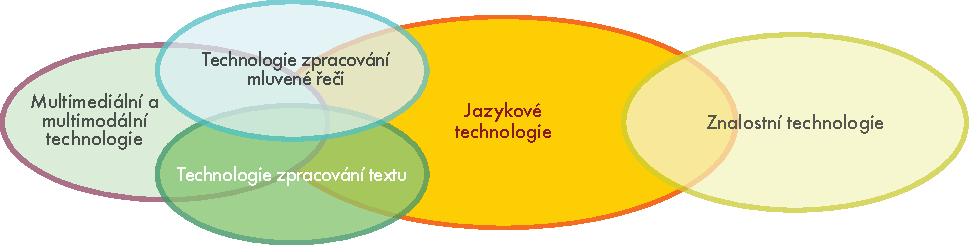
\includegraphics[width=\textwidth]{../_media/czech/language_technologies}
  \caption{Jazykové technologie}
  \label{fig:ltincontext_en}
  \colorrule{grey3}{\textwidth}{1.5pt}
\end{figure*}
Velké části jazykových technologií proto nelze zařadit ani pod technologii mluvené řeči, ani textu. Mezi ně patří technologie, které spojují jazyk a myšlení. Obrázek vpravo ukazuje oblast jazykových technologií. V rámci komunikace směšujeme jazyk s jinými způsoby komunikace a jinými informačními zdroji. Kombinujeme „řeč“ s gesty a výrazy obličeje. Digitální texty mohou obsahovat obrázky, grafy, zvuky apod. Filmy mohou obsahovat jazyk v mluvené i psané formě. Řečové a textové technologie se tedy překrývají a vzájemně ovlivňují s mnoha dalšími technologiemi, které usnadňují zpracování multimodální komunikace a multimediálních dokumentů.\\
V dalším textu popíšeme architekturu typického systému jazykových technologií. Následně podáme přehled základních aplikačních oblastí a stručně shrneme situaci jazykových technologií ve výzkumu a vzdělávání v ČR. Tabulka v závěru této části poskytuje vyhodnocení situace v nástrojích a datových zdrojích jazykových technologií z několika aspektů, jako je např. dostupnost, vyzrálost a kvalita.
\begin{figure*}[b]
  \colorrule{grey3}{\textwidth}{1.5pt}
  \center
  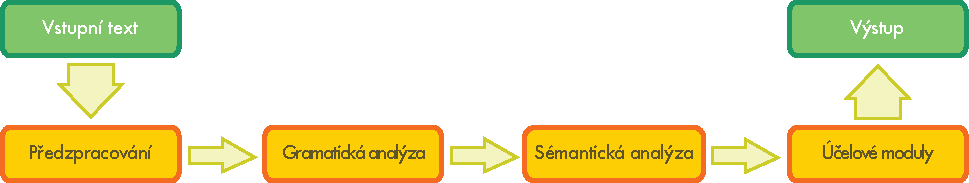
\includegraphics[width=\textwidth]{../_media/czech/text_processing_app_architecture}
  \caption{Typická architektura aplikací pro zpracování textu}
  \label{fig:textprocessingarch_en}
  \colorrule{grey3}{\textwidth}{1.5pt}
\end{figure*}
\subsection{Architektura aplikací}

Typické softwarové aplikace pro zpracování jazyka se skládají z komponent, které zohledňují různé aspekty jazyka a aspekty úlohy, kterou automatizují. Obrázek 2 znázorňuje vysoce zjednodušenou architekturu systému pro zpracování textů. První tři moduly se týkají struktury a významu textového vstupu:
\begin{enumerate}
  \item Předzpracování: čištění dat; odstranění formátování; detekce vstupního jazyka atd.
  \item Gramatická analýza: nalezení slovesa a jeho doplnění atd.; analýza struktury věty.
  \item Sémantická analýza: desambiguace významu (Jaký je správný význam slova „zámek“ v daném kontextu?); určování koreferenčních vztahů (jako „ona“, „jeho auto“, aj.); počítačová reprezentace významu věty.
\end{enumerate}
Specializované moduly následně provádějí mnoho různých úloh, jako je např. automatické shrnutí vstupního textu, databázové dotazy.

\subsection{Základní aplikační oblasti}

Dále rozebíráme hlavní aplikační oblasti jazykových technologií, jako je kontrola pravopisu, webové vyhledávání, hlasové ovládání a strojový překlad. Oblasti zahrnují aplikace a základní technologie, např.\\
\begin{itemize}
  \item oprava pravopisu,
  \item autorská podpora,
  \item počítačem podporovaná výuka jazyků,
  \item vyhledávání informací,
  \item extrakce informací,
  \item shrnutí textů,
  \item odpovídání na otázky,
  \item rozpoznávání řeči,
  \item syntéza řeči.
\end{itemize}
Pro každou aplikační oblast ilustrujeme vybrané moduly různých architektur, které záměrně popisujeme zjednodušeně.

\subsubsection{Jazyková kontrola}
\begin{figure*}[t]
  \colorrule{grey3}{\textwidth}{1.5pt}
  \center
  
\includegraphics[width=\textwidth]{../_media/czech/language_checking}
  \caption{Jazyková kontrola (vlevo: pravidlový přístup, vpravo: statistický přístup)}
  \label{fig:langcheckingaarch_en}
  \colorrule{grey3}{\textwidth}{1.5pt}
\end{figure*}
Morfologické a syntaktické vlastnosti češtiny představují velkou výzvu jak pro kontrolu překlepů, tak i pro kontrolu gramatické správnosti českých textů. Ačkoli již existují nástroje pro oba typy kontrol (první nástroje na kontrolu překlepů byly vyvinuty na začátku 90. let; vývoj prvního gramatického korektoru pro Microsoft Office trval mnohem déle, uživatelé se s ním mohli seznámit až v roce 2005), zůstává stále mnoho témat čekajících na efektivní řešení.\\
Existující nástroje na kontrolu překlepů pro češtinu jsou založeny na slovníku lemmat, zkombinovaném se sadou morfologických pravidel dovolujících analýzu nebo generování všech správných slovních forem. Ačkoli se tento jednoduchý postup zdá vyhovující, má dvě podstatné nevýhody. První z nich se týká překlepů, jež jsou ve skutečnosti správnými slovními tvary, které jsou nesprávné pouze v daném kontextu. V důsledku izolovaného zpracovávání jednotlivých slovních tvarů z textu je prakticky nemožné takovéto chyby objevit, proto by bylo velmi užitečné vyvinout pokročilejší algoritmy kontextové detekce chyb. Druhou nevýhodou je neschopnost rozeznat opravdové překlepy a ty slovní tvary, které jsou sice správné, ale nejsou obsaženy ve slovníku. Taková slova budou vždy existovat například v důsledku přirozeného obohacování slovní zásoby nově vytvořenými nebo přejatými slovy, novými vědeckými a odbornými termíny apod. Schopnost zachycovat tato slova by kontrolu překlepů pozvedla na kvalitativně novou úroveň.\\
Již v minulosti došlo k určitým pokusům podrobit kontrolu překlepů v závislosti na kontextu. Například jednou z nejčastějších chyb v češtině je použití špatné formy osobního zájmena „já“ v genitivu, dativu, akuzativu a lokálu. Obě formy používané v těchto pádech, jmenovitě „mě“ (gen., ak.) a „mně“ (dat., lok.), v mluvené řeči splývají a i proto je pisatelé velmi často nevhodně zaměňují. Automatické určení správného tvaru s ohledem na daný kontext teoreticky vyžaduje úplnou syntaktickou analýzu dané věty, protože správný pád obvykle nemůže být určen, aniž bychom brali ohled na syntaxi a slovesnou valenci. Tento fakt je výzvou pro vývoj sofistikovanější gramatické kontroly.\\
Řešení implementované v editoru Microsoft Word využívá skutečnosti, že zájmena v češtině téměř vždy bezprostředně následují za předložkou. Pokud se tato předložka váže pouze s jediným pádem (jako např. předložka „k“, „ke“), potom může být správný tvar zájmena určen s téměř 100\% spolehlivostí na základě tohoto místního kontextu. Nástroj Automatické opravy editoru MS Word proto obsahuje seznam předložek, které mají tuto vlastnost, v kombinaci se správným tvarem zájmena.\\
Tento příklad ukazuje, že další výzkum podobných morfologických či syntaktických vlastností může pomoci podstatně zlepšit kvalitu kontextové kontroly překlepů.\\
Čeština představuje ještě tvrdší oříšek pro gramatickou kontrolu, než je tomu u kontroly překlepů. Jde o jazyk s vysokým stupněm volnosti slovosledu, a proto je velmi obtížné na ni uplatnit metodu kontroly chybových vzorků v omezeném kontextu, která představuje standardní přístup pro jazyky s pevnějším slovosledem jako např. pro angličtinu. Pořadí slov ve správné české větě samozřejmě není úplně libovolné a určitá pravidla existují (například české příklonky mají zpravidla pevnou pozici ve větě), na druhou stranu ale volnost slovosledu v některých případech dokonce umožňuje odtrhnout shodný přívlastek od řídícího podstatného jména a umístit jej ve větě téměř libovolně, jako například v často citovaných příkladech z poezie \textit{Vánoční nadešel čas} a \textit{Hrdliččin zval ku lásce hlas}. Takové konstrukce, nazývané vzdálené závislosti nebo také neprojektivní konstrukce, představují velký problém pro jakoukoli kontrolu gramatické správnosti. Výzkum Pražského závislostního korpusu, syntakticky označkovaného souboru českých vět, ukázal, že asi 14\% vět z korpusu obsahuje alespoň jednu neprojektivní konstrukci. Tento počet jasně naznačuje, že tento jev nemůžeme ignorovat. Neprojektivní konstrukce ztěžují gramatickou kontrolu ještě z jednoho důvodu. Skutečnost, že závislé slovo může být ve větě umístěno i velmi daleko od svého řídicího slova, také stírá rozdíl mezi správnými a nesprávnými větami. Ukažme si tento jev pomocí následujícího příkladu:
\begin{itemize}
\item[] \textit{Které děvčata chtěla dostat šaty?}
\end{itemize}
Tuto větu můžeme buď považovat za syntakticky správnou, ale neprojektivní, s významem \textit{Které šaty chtěla děvčata dostat?}, nebo jako syntakticky nesprávnou, ale projektivní větu, ve které je chyba ve tvaru tázacího zájmena \textit{Které} (správný tvar je samozřejmě \textit{Která}). Vyřešit tuto víceznačnost je prakticky nemožné – neprojektivní konstrukce jsou integrální součástí češtiny a jejich přítomnost ve větě neznamená nic neobvyklého.
Syntaktická složitost neprojektivních konstrukcí v češtině je dokonce vyšší, než by mohl předchozí příklad napovídat. Jednoduchá česká věta může obsahovat více než jednu takovou konstrukci, jako např. věta:
\begin{itemize}
\item[] \textit{Tuto knihu jsem se mu rozhodl dát k narozeninám.}
\end{itemize}
Schéma přítomné v tomto příkladu, jmenovitě kombinace určitého a neurčitého slovesného tvaru s navzájem promíchanými závislými větnými členy, je v češtině velmi produktivní a teoreticky dovoluje vytvářet věty s prakticky libovolným počtem neprojektivních konstrukcí v jedné klauzi.
Ačkoli neprojektivní konstrukce představují pro kontrolu gramatické správnosti velký problém, protože na ně nestačí jednoduché metody odhalování chybných lokálních vzorků, nejsou v češtině jedinou syntaktickou výzvou. Přinejmenším stejně významnou překážkou je jiná syntaktická vlastnost češtiny – její schopnost vynechat podmět věty, pokud je z kontextu jasné, co jím má být. Podívejme se na ještě jeden příklad:
\begin{itemize}
\item[]\textit{Sportovci házely plyšáky.}
\end{itemize}
Tato věta je syntakticky nesprávná v typickém čtení, protože obsahuje neshodu v rodě mezi podmětem (\textit{sportovci} – rod mužský životný) a přísudkem (\textit{házely} – rod ženský nebo mužský neživotný). Situace se ale změní, pokud upravíme kontext následujícím způsobem:
\begin{itemize}
\item[]\textit{Dívky křičely. Sportovci házely plyšáky a rozhodčím shnilá rajčata.}
\end{itemize}
Skutečnost, že podmět může být z věty vynechán, výrazně ztěžuje existujícím nástrojům na kontrolu gramatické správnosti nalezení jednoho z nejčastějších typů gramatických chyb v češtině, neshody mezi podmětem a přísudkem. Dalšího vylepšení těchto nástrojů proto může být dosaženo pouze, pokud budeme chyby hledat v širším kontextu než v rámci jedné věty. Tento přístup však představuje velký úkol pro další výzkum.

Ačkoli první generace kontrolních jazykových nástrojů pro češtinu existuje, u ostatních nástrojů je situace horší. Například v oblasti autorské podpory existuje absolutní nedostatek nástrojů. To je způsobeno do určité míry skutečností, že čeština je obvykle cílovým a nikoli zdrojovým jazykem pro technickou dokumentaci nejrůznějších výrobků. Proto není potřeba takovýchto nástrojů tak naléhavá, jako je tomu u větších jazyků. Přesto však potřeba těchto a podobných nástrojů v budoucnu poroste a výzkum v oblasti zpracování přirozeného jazyka bude stále důležitější.
  
\subsubsection{Webové vyhledávání}
\begin{figure*}[htb]
  \colorrule{grey3}{\textwidth}{1.5pt}
  \center
  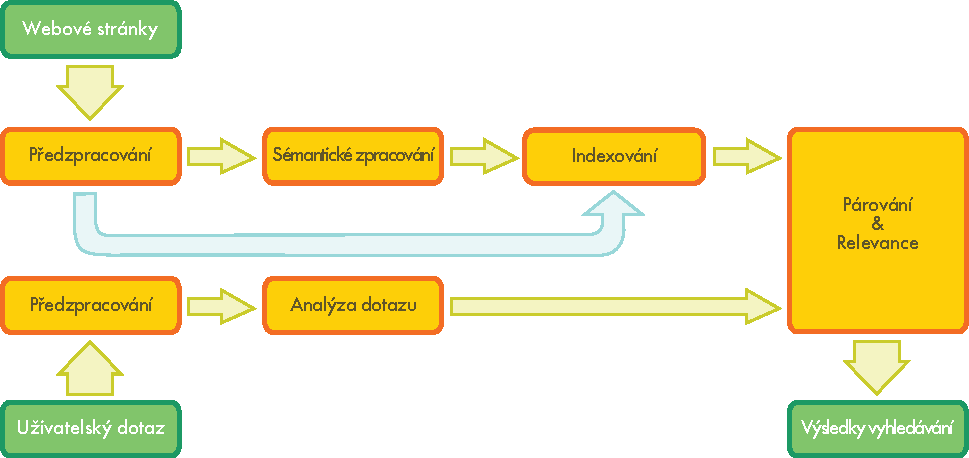
\includegraphics[width=\textwidth]{../_media/czech/web_search_architecture}
  \caption{Architektura webového vyhledávání}
  \label{fig:websearcharch_en}
  \colorrule{grey3}{\textwidth}{1.5pt}
 \end{figure*}
V České republice se tradičně hojně využívají domácí internetové vyhledávače. V současné době česká internetová populace nejčastěji využívá Seznam.cz, Google.com, Morfeo.cz a Jyxo.cz. Z toho vidíme, že situace je poněkud odlišná od ostatních zemí, kde má Google.com 80\% většinu. Na domácím trhu je dostatek prostoru jak pro vylepšení existujících vyhledávačů pomocí spolupráce akademického světa s průmyslem, tak i pro případné uvedení nové služby, zejména pokud by byla omezena na konkrétní obor či úkol, například zodpovídání otázek.

Pokud je nám známo, výsledky Googlu jsou považovány za nejrelevantnější. Google zahájil svůj provoz v roce 1998 a od té doby se příliš nezměnilo ani uživatelské rozhraní pro zadávání otázek, ani forma zobrazování výsledků. Příběh úspěchu vyhledávače Google ukazuje, že s využitím efektivních indexovacích technik a s dostatkem dat k dispozici může ryze statistický přístup vést k uspokojivým výsledkům.\\
Ovšem při složitějších informačních potřebách je nutno do vyhledávacích nástrojů zapojit hlubší lingvistickou znalost. Například pokud dotaz do vyhledávače tvoří celá věta namísto seznamu klíčových slov, je pro relevantní odpověď potřeba analyzovat dotyčnou větu na syntaktické a sémantické úrovni, jakož i mít k dispozici index umožňující rychlé poskytování relevantních dokumentů.
Kupříkladu si představme, že uživatel vloží otázku „Dej mi seznam všech firem, které během posledních pěti let pohltila jiná firma.“ S jednoduchým přístupem založeným na klíčových slovech se v tomto případě daleko nedostaneme. Výsledky může zlepšit rozšíření seznamu klíčových slov o synonyma, například s využitím ontologického jazykového zdroje WordNet. Ovšem pro uspokojivou odpověď je nezbytná hlubší analýza dotazu. Například při využití syntaktického parseru pro analýzu gramatické struktury věty můžeme určit, že uživatele zajímají firmy, které byly pohlceny, nikoli ty, které někoho/něco pohltily. Rovněž musíme zpracovat výraz „posledních pěti letech“, abychom správně vyhodnotili, které roky to jsou.\\
V češtině je analýza věty poněkud složitější, protože se musíme vyrovnat, jak už bylo řečeno, s bohatou morfologií a volným slovosledem. Domácí vyhledávače již v sobě většinou obsahují morfologickou analýzu nebo alespoň část její funkcionality, ovšem kvalita těchto nástrojů se různí.\\
A konečně, zpracovaný dotaz je třeba porovnat s velkým množstvím nestrukturovaných dat, abychom nalezli informace, které uživatel hledá. Tento úkol zahrnuje získání a ohodnocení relevantních dokumentů. Abychom mohli vytvořit požadovaný seznam firem, musíme také mít informace o tom, že určité shluky písmen jsou názvy firem. Tento typ informace se dá získat pomocí rozpoznávače pojmenovaných entit.\\
Úkol je možno ještě zesložitit, pokud chceme vyhodnocovat dotaz nad dokumenty psanými v jiném jazyce. Pro vícejazyčné vyhledávání je třeba automaticky přeložit dotaz do všech dostupných zdrojových jazyků a získanou informaci přeložit zpět do cílového jazyka. Tento úkol opět zahrnuje lingvistickou analýzu. Pro uživatele se specifickými informačními potřebami může rozšíření dotazu vyžadovat dodatečné zdroje informací jako například doménově specifickou ontologii reprezentující vztahy mezi jednotlivými pojmy.

Vzrůstající podíl sdílení dat v netextových formátech rovněž zvyšuje poptávku po službách umožňujících multimediální vyhledávání, tj. vyhledávání v obrázcích, audio a video datech. Pro audio a video soubory je tudíž potřeba zapojit modul pro rozpoznávání řeči, který převede mluvenou řeč do textové či fonetické reprezentace, ve které pak můžeme vyhledávat odpovědi na uživatelovy dotazy.

\subsubsection{Jazykové technologie}

Obecné rozpoznávání mluvené češtiny je stále v začátcích. Jednoduché aplikace s malým slovníkem a gramatikou dosahují vysoké spolehlivosti i díky jednoduchému fonetickému systému češtiny. Hlavním problémem velkých aplikací s rozsáhlým slovníkem a obecnějším jazykovým modelem češtiny je vysoký počet slovních tvarů, relativně volný slovosled a nespisovné tvary. Tyto zvláštnosti zatím brání dosažení podobné úspěšnosti rozpoznávání s pomocí klasických statistických metod, jako existují pro angličtinu.
\begin{figure*}[htb]
  \colorrule{grey3}{\textwidth}{1.5pt}
  \center
  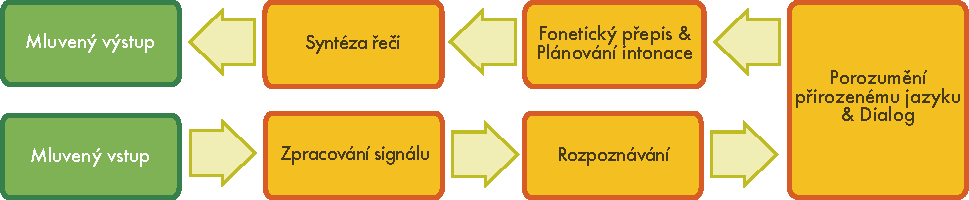
\includegraphics[width=\textwidth]{../_media/czech/simple_speech-based_dialogue_architecture}
  \caption{Architektura jednoduchého hlasového dialogu}
  \label{fig:dialoguearch_en}
  \colorrule{grey3}{\textwidth}{1.5pt}
\end{figure*}
Existuje několik komerčních systémů s velkými slovníky (SpeechTech s.r.o.\cite{Note11}, OptimSys, s.r.o.\cite{Note12}, NewtonTechnologies, a.s.\cite{Note13}), které však pracují buď jako diktovací aplikace s velmi kvalitním zvukovým vstupem, nebo mají silně omezenou jazykovou doménu např. na sportovní nebo parlamentní přenosy. Je možné zakoupit samostatný modul rozpoznávání mluvené řeči s podporou rozhraní Media Resource Control Protocol, který umožňuje začlenění této technologie i do jiných aplikací. Firmy nabízejí aplikace generující off-line přepis multimediálních archivů a jejich prohledávání. Všechny tyto programy mají relativně dobré konfigurační možnosti, ale nespadají do oblasti open-source. K vývoji rozpoznávače mluvené češtiny jako open-source v současnosti chybí open-source akustická data, která by umožnila přípravu volně dostupných akustických modelů nezávislých na mluvčích. Nástroje a knihovny nutné pro přípravu takového systému jsou k dispozici, ale navíc stále chybí spolehlivější metoda rozpoznávání pro češtinu se všemi jejími slovními tvary a volným slovosledem.\\
Syntéza mluvené češtiny má několik komerčních systémů na dobré úrovni (Eris\cite{Note11}, Acapela Group\cite{Note14}), navíc i open-source aplikace pro syntézu hlasu, bohužel zatím s nižší kvalitou (Festival Czech\cite{Note15}, Epos TTS System\cite{Note16}, MBROLA\cite{Note17}).\\
Moduly syntézy řeči jsou připravené k integraci do interaktivních systémů, které podporují mnoho otevřených standardů. K vytvoření open-source aplikací pro syntézu hlasu s vysokou kvalitou opět chybí volně dostupné hlasové nahrávky mluvčích.\\
Dialogové systémy jsou také ve svých začátcích díky závislosti na předchozích dvou technologiích. Český dialogový systém bez omezení je cílem společného výzkumu více univerzit, oddělení mluvené řeči pracují na mnoha projektech, což jim umožňuje sestavit jednoduché dialogové systémy zahrnující většinu hlasových technologií. Současný výzkum mluvené češtiny se zaměřuje na zlepšení jazykového modelu.  Kromě ověřené metody navýšení množství trénovacích jazykových dat, které vyžaduje časově náročné přepisování, se hledají specifické postupy pro češtinu. Jeden směr výzkumu se snaží o konverzi mluvené češtiny do formální psané podoby, pro které již existují spolehlivější metody založené na textových korpusech. Kromě jednoduchých případů, např. záměny koncovek obecné češtiny jejich spisovnoou formou, musí metoda řešit i náhradu celých slovních frází jejich správnou formou. Podobným způsobem jsou odstraňovány další jevy spontánní řeči, mezi něž patří výplňová slova, opravy a potvrzovací signály posluchače.

Druhý směr výzkumu se zaměřuje na vývoj syntaktických a sémantických analyzátorů vyvíjených s pomocí anotovaných stromových korpusů psané a mluvené češtiny.  Ve spojení s morfologickou analýzou by tato metoda měla pomoci se zpracováním volného slovosledu a velkého množství slovních tvarů.\\
Výzkum syntézy mluvené češtiny se snaží vyvinout přirozenější hlasy. Naděje se vkládá do pokročilejší syntaktické a sémantické analýzy vstupních textů, která by měla podstatně zlepšit přirozenost promluvy.

\subsubsection{Strojový překlad}

Nápad využít digitální počítače pro překlad přirozených jazyků pochází od A. D. Boothe z roku 1946. V padesátých letech 20. st. a po určité pauze opět od let osmdesátých bylo do tohoto směru výzkumu investováno značné množství prostředků. I přesto strojový překlad (machine translation, MT) dodnes nesplňuje vysoká očekávání, jak byla formulována v prvních letech.

Na území České republiky nápad překladu prováděného počítači velmi zaujal lingvisty a matematiky záhy po prvních pokusech s překladem ve světě (1954 v USA, 1955 v Sovětském svazu). V lednu 1960 byl proveden první pokus přeložit několik vět z angličtiny do češtiny na počítači SAPO první generace, který byl vyroben v tehdejším Československu. Za pokusy stála malá skupina badatelů z Karlovy univerzity a Výzkumného ústavu matematických strojů. Univerzitní skupina pokračovala ve vývoji metod strojového překladu i dále a pro počítače druhé generace (z NDR a SSSR) byly vytvořeny experimentální pravidlové systémy pro anglicko-český a česko-ruský překlad. Systémy byly omezeny na úzkou doménu textů a sloužily především jako potvrzení správnosti formálně zapsaných gramatických pravidel. V devadesátých letech 20. st. byl navržen prototyp překladu mezi blízkými jazyky, konkrétně mezi češtinou a slovenštinou, systém Česílko\cite{Note18}. V praxi se tento systém bohužel nepoužívá zejména kvůli náročné údržbě. Následný výzkum vkládá více nadějí do statistických metod nebo kombinace statistických a pravidlových metod.\\
V základní implementaci strojový překlad nahrazuje jednotlivá slova zdrojového jazyka slovy z jazyka cílového. Takto primitivní přístup lze s úspěchem použít jen ve velmi úzkých oblastech s jednoduchým vyjadřováním, např. v předpovědích počasí (srov. systém METEO\cite{Note19}). Pro překlad méně standardizovaných textů je nutné zohlednit větší úseky textu (fráze, věty nebo i celé pasáže). Hlavní problém pak představuje víceznačnost lidské řeči projevující se na vícero úrovních, např. u lexikálního obsazení jde o tzv. word sense disambiguation (WSD), u větného rozboru o určení řídícího členu pro předložkové skupiny (PP-attachment).
\begin{figure*}[htb]
  \colorrule{grey3}{\textwidth}{1.5pt}
  \center
  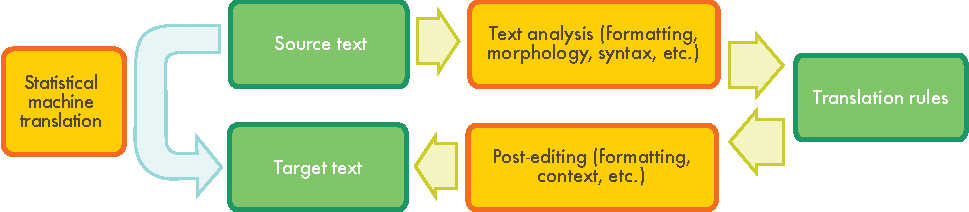
\includegraphics[width=\textwidth]{../_media/english/machine_translation}
  \caption{Strojový překlad (nahoře: statistický přístup, dole: pravidlový přístup)}
  \label{fig:mtarch_en}
  \colorrule{grey3}{\textwidth}{1.5pt}
\end{figure*}
Jeden z možných přístupů k úloze se opírá o lingvistická pravidla. Pro překlad mezi příbuznými jazyky stačí překlad slovo od slova. Pravidlové systémy naproti tomu často vstupní text rozebírají a vytvářejí dočasnou, symbolickou reprezentaci, z níž je teprve výsledný text generován. Úspěch těchto metod velmi závisí na dostupnosti rozsáhlých slovníků obsahujících morfologickou, syntaktickou i sémantickou informaci o slovech, a též souborech gramatických pravidel pečlivě navržených zkušeným lingvistou.\\
Pro češtinu existuje několik komerčních i akademických systémů založených na slovnících a pravidlech. Jeden z nich se opírá o lingvistickou teorii pocházející z 60. let 20. st. Systém sleduje načrtnuté rozdělení úlohy na fáze analýzy, transferu a syntézy. I přes lingvistickou adekvátnost tohoto přístupu systém stále trpí řadou praktických nedostatků, např. relativně velkou chybovostí nástrojů pro automatický větný rozbor nebo narůstající výpočetní složitostí překladu slov, při kterém je třeba zohlednit všechny relevantní informace z kontextu.\\
Koncem 80. let 20. st. se s levnější a větší výpočetní silou počítačů zájem přesunul ke statistickým modelům. Tyto modely jsou automaticky vybudovány na základě analýzy dvojjazyčných souborů textů, jako je např. paralelní korpus Europarl obsahující zápisy z jednání Evropského parlamentu v 21 evropských jazycích. (Čeština byla přidána teprve nedávno a data pro češtinu jsou stále o několik řádů menší než pro zavedené jazyky.) Při dostatku dat pracuje statistický překlad pro přibližné pochopení textu dostatečně dobře. Na rozdíl od pravidlových metod však často generuje gramaticky nesprávný výstup. Silnou stránkou statistického přístupu je pak, kromě ušetřené námahy při přípravě pravidel, často plně automatické zachycení specifických frází včetně idiomů. Stačí, aby byly pokryty trénovacími daty. Právě dostupnost rozsáhlých objemů dvojjazyčných textů je klíčem k úspěšnému statistickému překladu. Pro češtinu jsou v současné době vytvářeny paralelní korpusy s několika dalšími jazyky. Největší soubor dat CzEng\cite{Note20}, celkově několik milionů dvojic vět, je dostupný pro češtinu a angličtinu. Tento korpus zahrnuje např. evropské právní dokumenty, novinové texty, technickou dokumentaci a elektronicky dostupné knihy. Nejtěžší problém při přípravě takového korpusu je tzv. zarovnání, tj. nalezení odpovídajících si dvojic úseků textu. Nejen že přiřazení slov slovům nelze často ani teoreticky provést správně pro odlišnosti v tvarosloví a skladbě zarovnávaných jazyků, často je obtížné přiřadit k sobě správně celé věty nebo i celé dokumenty. Proces zarovnání musí být navíc zcela automatický; s ohledem na objem textů je ruční zpracování vyloučeno. Jazyky s bohatou morfologií jako čeština pro současné systémy strojového překladu představují zvlášť obtížnou úlohu. Systém musí nejen vybrat správné slovo, ale navíc dobře zvolit gramatická pravidla pro stanovení jeho konkrétního tvaru s ohledem na kontext ve větě. V současné době jen velmi málo statistických systémů explicitně pracuje s morfologickou reprezentací, a proto často narazí na nedostatek dat: ani v největších paralelních korpusech nelze očekávat, že uvidíme slovo ve všech jeho potřebných tvarech.

Vzhledem k tomu, že klady a zápory statistických a pravidlových systémů se do značné míry doplňuji, panuje dnes víceméně souhlas, že je dobré je kombinovat do hybridních metod. Kombinace je přitom možné provádět několika způsoby. Nejjednodušší je přeložit větu oběma systémy a (strojově) následně zvolit jednu z těchto odpovědí. Pro delší věty však nelze očekávat dobrý výsledek. Vhodnější přístup proto kombinuje nejlepší úseky z výstupů několika systémů. To je ovšem obtížnější, protože často je těžké strojově poznat, které části výstupů si odpovídají, nehledě na nutnost správně je spojit do výstupu jediného.
Alternativní, a samozřejmě obtížnější, je možnost navrhnout nový přístup k překladu, který obě metody integruje. Je například možné pravidlový systém obohatit modulem pro automatickou extrakci pravidel z dat nebo je možné statistický systém doplnit gramatickými pravidly.\\
Zcela samostatnou otázku pak představuje úloha vyhodnocování kvality strojového překladu, ať již ručně nebo strojově. Zkušenosti ukazují, že různé přístupy překladu jsou různě úspěšné v různých ohledech: pravidlové systémy mají větší šanci zachovat význam, statistické systémy produkují výstup, který je plynulejší na úrovni krátkých sousloví. Například v úloze odpovídání na otázky sice lokální plynulost ve srovnání s jinými systémy dobře působí na uživatele, ale přesnost odpovědí může utrpět. Automatické vyhodnocování kvality (založené na porovnání výstupu MT s lidským překladem) je zcela zásadní pro vývoj zejm. statistických modelů. Ukazuje se však, že většina automatických hodnocení kvality je nespolehlivá, a to ještě výrazněji pro jazyky s bohatou morfologií. Pro vývoj systémů strojového překladu by též velmi pomohly nástroje, které klasifikují a podrobně zobrazí chyby ve výstupu.

\subsection{Informační managment/Jazykové technologie „v zákulisí“}

Vytváření aplikací jazykových technologií zahrnuje celou řadu podúloh, které sice komunikují s uživatelem omezeně, ale poskytují zásadní funkcionality systémů. Tím formulují důležitá výzkumná témata, ze kterých vznikají samostatné disciplíny komputační lingvistiky.

Například, zodpovídání otázek (question asnwering, QA) je aktivní oblastí výzkumu, pro kterou jsou připravovány anotované korpusy, organizovány soutěže atd. Cílem je posunout se od hledání na základě klíčových slov (pro které vyhledávací stroje vrací kolekci potencionálně relevantních dokumentů) k postupu, kdy uživatel položí konkrétní otázku a systém vrátí jasnou odpověď:\\
\begin{itemize}
\item[] \textit{Otázka: V kolika letech vystoupil Neil Armstrong na Měsíc?}
\item[] \textit{Odpověď: 38.}
\end{itemize}
Zatímco toto zřetelně souvisí s výše popsanou oblastí webového hledání, zodpovídání otázek dnes zastřešuje hlavně výzkum otázek, a sice jaké typy otázek by měly být rozlišeny a jakým způsobem by měly být zpracovávány; jak má být množina dokumentů, která teoreticky obsahuje odpověď, analyzována a porovnávána (vracejí dokumenty rozporuplné odpovědi?); jak může být určitá informace - odpověď - spolehlivě extrahována z dokumentu bez přehnaného ignorování kontextu; atd.

To pro změnu souvisí s úlohou extrakce informací (information extraction, IE), s oblastí, která byla nesmírně populární a významná v době „statistické otočky“ v počítačové lingvistice na počátku 90. let minulého století. Cílem IE je identifikace specifických informací ve specifických třídách dokumentů, např. detekce klíčových postav při převzetí společnosti, které jsou uváděny v novinových článcích. Jiným příkladem je podávání zpráv o teroristických incidentech, kdy úkolem je mapovat text na šablonu vymezující pachatele, cíl, čas, místo incidentu a výsledek incidentu. Doménově řízené vyplňování šablon je hlavní charakteristikou IE, což ji řadí mezi příklady technologií „v zákulisí“. Je dobře vymezenou výzkumnou oblastí, ale z praktického hlediska musí být začleněna do vhodného aplikačního prostředí.\\
Dvě „mezní“ oblasti, které někdy vystupují samostatně a někdy jako podpůrné komponenty, jsou shrnutí textu (text summarization, TS) a generování textu (text generation, TG). Aplikace TS dělají z delšího textu kratší text a jsou nabízeny například jako funkcionalita editoru MS Word. Většinou vycházejí ze statistiky a postupují tak, že nejdříve v textu identifikují „důležitá“ slova (tj. např. slova, která se vyskytují často v textu, ale podstatně méně často v obecném užívání jazyka) a následně určují věty, které většinu těchto „důležitých“ slov obsahují. Tyto věty jsou poté použity na sestavení shrnutí. V tomto zdaleka nejpopulárnějším postupu znamená TS extrakci vět, tj. text je zredukován na podmnožinu vět. Všechny komerční systémy tento postup aplikují.
Alternativním přístupem je syntéza nových vět, tj. sestavení shrnutí z vět, které se v dané formě nemusí ve zdrojovém textu vyskytovat. Tento postup vyžaduje hlubší porozumění textu, a proto je méně robustní. Ba co víc, je do značné míry zaměřen na určitou doménu nebo žánr textu, protože je třeba specifických znalostí k dalšímu kroku abstrakce zdrojového textu směrem k jeho obsahu. Sestavení shrnutí pak odpovídá generování textu, tj. vytvoření nového textu buď z jiného textu (viz shrnutí), nebo z netextových dat. To může být využito ke generování zpráv o vývoji určitých dat v čase - např. generování zpráv o počasí a kvalitě vzduchu, shrnutí lékařských diagnóz aj. Aplikace TG většinou nejsou samostatnou aplikací, bývají začleněny do větších softwarových produktů, jako je např. informační systém kliniky, ve kterém jsou shromažďovány, ukládány a zpracovávány údaje o pacientech, a generování zpráv je jednou z jeho funkcionalit.

V České republice je několik výzkumných skupin, které pracují na mezinárodních (rozuměj anglických) aplikacích. Pouze část výzkumného úsilí je zaměřena na češtinu, a sice existují dílčí komponenty počítačového zpracování češtiny, jako jsou kontrola překlepů, korpusy, morfologické desambiguátory, valenční slovníky, analyzátor českých kolokací (Word Sketch Engine for Czech vyvinutý na Masarykově univerzitě v Brně (\cite{Horak2009})), rozpoznávání a generování mluvené řeč; komplexní systém použitelný v průmyslu dosud neexistuje.\\
Pokud je nám známo, pro češtinu existuje jediný dialogový systém (aplikace QA), a sice UIO (Umělá inteligence opice), vyvinutý na Masarykově univerzitě v Brně (\cite{Svoboda2003}). UIO prohledává databáze a internet a v aktuálně dostupné verzi může být použit pro hledání ve vlakových a autobusových jízdních řádech, v programech kin a divadel, v kurzovních lístcích, v kalendářích a v Diderotově encyklopedii. Pro všechny uvedené domény vykazuje systém 80\% úspěšnost v zodpovídání otázek. Konkurenční systém, dosud bez jména, vzniká na Západočeské univerzitě.\\
Jednoduchý dialogový systém vznikl v Ústavu formální a aplikované lingvistiky, UK MFF ve spolupráci s Katedrou kybernetiky Západočeské univerzity a v omezené míře s některými partnery projektu FP6 Companions\cite{Note21}. Avatar konverzuje se seniorem o archivu jeho osobních fotografií a o životních zážitcích (\cite{Ptacek2010}, \cite{Romportl2010}, \cite{GruberTihelka2010}).\\
Text-Mining Research Group na Západočeské univerzitě vyvíjí tzv. User Profile Generation system (\cite{Grolmus2003}). Tento systém provádí dolování informací z textu v dokumentech shromážděných a nahlížených uživatelem. Uživatelem schválené informace se využívají k doporučení konkrétních dokumentů pro další vyhledávání, stejně tak i pro odhad uživatelovy odbornosti v dané doméně. Tato aplikace může být použita jako softwarová podpora digitálních knihoven.\\
WebGen, vyvinutý na Masarykově univerzitě v Laboratoři vyhledávání a dialogu, (LSD lab\cite{Note22}), je dialogový systém, který pomáhá zrakově postiženým lidem generovat webové prezentace v češtině (\cite{BartelPlhak2008}).\\
Vysoké technické učení v Brně, Fakulta informačních technologií, Ústav počítačové grafiky a multimédií navrhl a implementoval klient-server software pro zpracování mluvené řeči\cite{Note23}, který doplňuje sémantické popisky do přepisů mluvené řeči (Speech Tagging, \cite{Smrz2010}). Klient komunikuje se serverem přes webové rozhraní, přes které se provádí nahrání a analýza zvukových nahrávek. Uživatel má možnost definovat a organizovat tzv. „tags“ („značky“), které jsou skupinami sémanticky blízkých klíčových slov. Pokud je nějaké klíčové slov nalezeno v nahrávce, je nahrávka označkována odpovídajícím způsobem. Tato služba by mohla být vhodná např. při krizovém řízení pro klasifikaci telefonních hovorů podle pronesených slov. Pokud je nám ale známo, k využití systému v reálných aplikacích doposud nedošlo.\\
Katedra kybernetiky Západočeské univerzity v Plzni vyvinula několik aplikací pro zpracování mluvené češtiny, jako je dialogový systém s vlakovými jízdními řády nebo dialogový systém pro registraci studentů ke zkouškám po telefonu (University Voice XML information systém).\cite{Note24} Její výzkumné skupiny vedou několik projektů zaměřených na asistenci sluchově postiženým lidem, např. překládání mezi češtinou a českou znakovou řečí.\\
Další užitečnou aplikací (opět vyvinutou v Plzni) je systém hlasového ovládání pro dentisty (\cite{Nagy2008}), který pracuje ve dvou režimech: v prvním režimu čte zprávu o zubu pacienta a ve druhém nahrává to, co lékař diktuje, a aktualizuje zprávu. Hlasové ovládání je zde nezbytné, protože lékař nemá během vyšetřování pacienta dovoleno se dotýkat obrazovky ani ovládání diktovacího zařízení.\\
Výzkumné skupiny Západočeské univerzity a ÚFAL UK MFF spolupracovaly v mezinárodním projektu MALACH (Multilingual Access to Large Spoken Archives a v hebrejštině znamená nebeský anděl), (\cite{Psutka2005}). Skupiny byly zodpovědné za rozpoznávání mluvené řeči a sémantickou indexaci výpovědí zaznamenaných v češtině a dalších slovanských jazycích. Univerzita Karlova je jedním z míst, ve kterých je možné vyhledávat v archivu výpovědí těch, kteří přežili holokaust. (Jiná přístupová místa se nacházejí ve Spojených státech, Německu, Maďarsku, Izraeli a Austrálii.)

Organizace Shoah Foundation Institute´s Visual History Archiv pořídila v letech 1994-1999 v 56 zemích a ve 32 jazycích téměř 52 tis. videonahrávek výpovědí. Většina rozhovorů jsou s přeživšími Židy, dále s politickými vězni, Romy a Sinty, Svědky Jehovovými, a dále s těmi, co přežili experimenty zušlechťování lidské rasy, homosexuály, zachránci a osvoboditeli a účastníky soudních procesů s válečnými zločinci.

Archiv je přístupný on-line přes rozhraní, které umožňuje uživatelům listovat výpověďmi a prohlížet je s využitím indexu 55 tis. klíčových slov a  frází. Pražské přístupové místo uchovává více než 500 výpovědí v češtině, každá výpověď trvá průměrně dvě hodiny. Další výpovědi musí být objednány on-line z jiných přístupových míst, což většinou trvá několik hodin.

\subsubsection{Miscelanea}

Ukazuje se, že posuzovat úroveň národního výzkumu a vývoje v oblasti jazykových technologií a zpracování řeči výhradně podle množství dostupných datových zdrojů a funkčních aplikací pro daný jazyk by bylo krajně zavádějící. Tak se udržuje začarovaný kruh: národní vlády i grantové agentury chtějí podporovat jen ty nejlepší výzkumné týmy. Nejlepšími týmy jsou podle scientometrických ukazatelů ty, které dosáhly největšího množství mezinárodně uznávaných publikací. Ovšem mezinárodních publikací se nesrovnatelně lépe dosahuje s mezinárodně zajímavým výzkumným tématem. Tematizujeme-li velké a strategické jazyky, jako je například angličtina, čínština nebo arabština, sebemenší pokrok je mezinárodně zajímavý a má tak naději na dobře hodnocenou publikaci. Naproti tomu stejný výsledek na jazyku, který běžně používá pouze malé společenství jeho rodilých mluvčích, má logicky mnohem menší mezinárodní dopad, a tudíž mnohem menší naději na prezentaci v prestižních médiích. Mezinárodně uznávaného hodnocení tak ve výzkumu malých jazyků zpravidla dosáhne jenom opravdový průlom v některé z mezinárodně řešených problematik. Takový nepochybný průlom je však ve vědě spíše svátkem než pravidlem. Navíc, jde-li o dobrý výsledek vázaný na problém jazykově specifický, je často nemožné ho přesvědčivě podat recenzentům, kteří daný jazyk neovládají, například v přísně omezeném rozsahu konferenčního abstraktu.\\
Dalším nepříznivým faktorem pro výzkum a vývoj jazykových technologií přímo na malých jazycích je fakt, že nejvíce oceňovanými řešeními jsou řešení nezávislá na konkrétním jazyku. Jejich komerční aplikace je totiž mnohem levnější než jazykově specifická řešení. Výsledky jednotlivých výzkumných týmů se nejlépe porovnávají na stejném jazyku. Nejobvyklejším cizím jazykem je pro Evropany angličtina. Kromě toho pro ni existují nejpočetnější a nejkvalitnější jazykové zdroje. Proto není nikterak překvapující, že evropský výzkum a vývoj jazykově nezávislých technologií vychází převážně z experimentů prováděných na angličtině.
V důsledku jmenovaných vlivů se národní týmy soustřeďují spíše na angličtinu než na svůj mateřský jazyk. To je třeba zohlednit při posuzování úrovně národního výzkumu v oblasti jazykových technologií a zpracování přirozeného jazyka. Chudý inventář jazykových zdrojů a chybějící aplikace pro daný jazyk neznamenají nutně špatnou úroveň oboru v dané zemi jako takového, ale naopak můžou být závažným příznakem chybějící vládní jazykové politiky. Pro jazyková společenství, která jsou příliš malá na to, aby výzkum a vývoj národních jazykových technologií byl ekonomicky zajímavý pro soukromý sektor. V těchto případech je cílená vládní podpora jazykových technologií pro národní jazyk naprosto nezbytná.

\subsection{Průmysl a programy jazykových technologií}

Průmyslový rozvoj jazykových technologií není v České republice zdaleka rozšířen, podnikání v oblasti jazykových technologií je spíše vzácné. Stejná situace je i ve vědeckých a výzkumných odděleních větších společností.

V současné době využívají webové vyhledávače a webové služby (Seznam, Centrum, Google aj.) morfologickou analýzu a lematizaci. Google nabízí tzv. frázový strojový překlad webových stránek i vlastních textů uživatelů z a do češtiny. Seznam nabízí dvoujazyčné on-line slovníky s češtinou na jedné straně a s angličtinou, němčinou, francouzštinou, španělštinou a ruštinou na straně druhé.Několik společností vytváří a publikuje dvoujazyčné elektronické slovníky jako aplikace pro MS Windows, případně Linux.\\
Většina z nich obsahuje morfologickou analýzu a/nebo lemmatizaci, některé z nich také ontologie. Na mobilních telefonech je možné používat českou verzi T9. Balíčky kancelářského softwaru (např. Microsoft Office 2010) zahrnují pro češtinu kontrolu překlepů, kontrolu pravopisu, někdy strojový překlad a rozpoznávání mluvené řeči (tj. zpracování hlasového vstupu).\\
Nahrávky telefonních hovorů a aplikace pro poskytování nápovědy/informací, které využívají automatické rozpoznávání mluvené řeči (ASR), zůstávají nevyužity. Proběhl sice pilotní projekt univerzitních skupin, které se ASR věnují (hlavně Západočeská univerzita v Plzni a Technická univerzita v Liberci), ale k širšímu průmyslovému využití těchto technologií doposud nedošlo.
Rozpoznávání mluvené češtiny komercializovala společnost Newton Technologies, coby spinoff Technické univerzity v Liberci. Většina vládou financovaných programů je spravována Grantovou agenturou České republiky (GAČR) s důrazem na základní výzkum. V roce 2009 byla založena Technologická agentura České republiky (TAČR) s ambicemi finančně podporovat aplikovaný výzkum. Domníváme se ale, že tato agentura doposud nefinancovala projekt zaměřený na jazykové technologie.

\subsection{Jazykové technologie ve výzkumu a vzdělávání --- LT research and education}

Pojmy „počítačová lingvistika“, „počítačové zpracování přirozeného jazyka“ a „rozpoznání mluvené řeči“ jsou podstatně starší než pojem jazykové technologie, alespoň z pohledu výzkumu a vzdělávání. Bez ohledu na terminologii, obory, které se věnují přirozenému jazyku, zahrnují i obory výzkumu a vzdělávání, jako je teoretická lingvistika, korpusová lingvistika, informatika, matematika, strojové učení aj.

V České republice působí několik institucí, které věnují svůj výzkum a výuku počítačovému zpracování přirozeného jazyka. Níže uvádíme jejich seznam včetně informací, na jaký podobor se zaměřují (PL – počítačová lingvistika, KL – korpusová l., TL – teoretická l., ASR – rozpoznávání mluvené řeči) a jaké studijní programy nabízejí.

%FIXME Can this be rewritten as text?
\begin{itemize}
\item[] \textbf{Univerzita Karlova v Praze}\\
  %\begin{itemize}
   Ústav formální a aplikované lingvistiky\\ (\textit{http://ufal.mff.cuni.cz}); PL, TL, ASR; Bc., Mgr., PhD.;\\
  Ústav českého národního korpusu\\ (\textit{http://ucnk.ff.cuni.cz/english/index.php}); KL; PhD.\\
  Ústav teoretické a komputační lingvistiky \\(\textit{http://utkl.ff.cuni.cz}); PL; PhD.;
  %\end{itemize}
\item[] \textbf{Vysoká škola ekonomická v Praze}\\  
  Katedra informací a znalostního inženýrství \\(\textit{http://kizi5.vse.cz}), získávání znalostí, sémantický web, ontologie; BSc, MSc, PhD;
\item[] \textbf{České vysoké učení v Praze}\\
  Katedra kybernetiky \\(\textit{http://cyber.felk.cvut.cz/}); robotika, umělá inteligence; Bc., Mgr., PhD.;\\
  Katedra teorie obvodů \\(\textit{http://noel.feld.cvut.cz/speechlab/start.php?page=projects\&lang=en\#2});  ASR; Bc., Mgr., PhD.
\item[] \textbf{Masarykova Univerzita v Brně}\\
  Laboratoř počítačového zpracování jazyka\\ (\textit{http://nlp.fi.muni.cz/en/nlplab}); PL, ASR;\\ 
  Ústav českého jazyka\\ (\textit{http://www.muni.cz/phil/211700?lang=en}); CL, TL; BSc, MSc, PhD;
\item[] \textbf{Vysoké učení technické v Brně}\\
  Skupina zpracování řeči \\(\textit{http://speech.fit.vutbr.cz/}); ASR;\\ 
  Výzkumná skupina automatického zpracování jazyka \\(\textit{http://www.fit.vutbr.cz/research/groups/nlp/index.php?lang=en}); CL; 
\item[] \textbf{Západočeská univerzita v Plzni}\\
  Katedra kybernetiky\\ (\textit{http://www.kky.zcu.cz/en}); ASR; Bc., Mgr., PhD.;
\item[] \textbf{Technická univerzita v Liberci}\\
  Laboratoř počítačového zpracování řeči \\(\textit{https://www.ite.tul.cz/speechlabe/}); ASR; 
\end{itemize}

Univerzita Karlova v Praze, Matematicko-fyzikální fakulta (UK MFF) nabízí evropský magisterský a postgraduální studijní program tzv. European Master Program in Language and Communication Technologies. Díky této aktivitě může UK MFF hostit zahraniční studenty, kteří jsou zároveň zdrojem impulsů pro zpracování dalších jazyků pro jejich české kolegy.\\
Výzkum přirozeného jazyka v privátní sféře není v ČR rozšířen a zabývají se jím spíše menší firmy (např. Lingea, Captaworks, Langsoft) a spinoffy založené univerzitními týmy (např. SpeechTech,- ZČU Plzeň, Phonexia – VUT Brno).\\
Studijní programy vzdělávacích institucí jsou zaměřeny jak na teoretické znalosti, tak i na aplikace. Bohužel, poptávka po odbornících těchto programů je v ČR nízká.

\subsection{Dostupné nástroje a zdroje pro češtinu}
  
Následující tabulka podává přehled aktuálního stavu dostupných jazykových technologií pro češtinu. Ohodnocení jednotlivých nástrojů a zdrojů je založeno na odborném odhadu expertů v daném oboru (0 nejhorší, 6 nejlepší). 

\begin{figure*}[htb]
\centering

\begin{tabular}{>{\columncolor{orange1}}p{.33\linewidth}@{\hspace*{6mm}}c@{\hspace*{6mm}}c@{\hspace*{6mm}}c@{\hspace*{6mm}}c@{\hspace*{6mm}}c@{\hspace*{6mm}}c@{\hspace*{6mm}}c}
\rowcolor{orange1}
 \cellcolor{white}&
 \begin{sideways}\makecell[l]{Množství}\end{sideways} &
 \begin{sideways}\makecell[l]{\makecell[l]{Dostupnost} }\end{sideways} &
 \begin{sideways}\makecell[l]{Kvalita}\end{sideways} &
 \begin{sideways}\makecell[l]{Pokrytí}\end{sideways} &
 \begin{sideways}\makecell[l]{Vyzrálost}\end{sideways} &
 \begin{sideways}\makecell[l]{Udržovatelnost}\end{sideways} &
 \begin{sideways}\makecell[l]{Adaptabilita}\end{sideways} \\ \addlinespace

\multicolumn{8}{>{\columncolor{orange2}}l}{\textcolor{black}{Jazykové technologie (nástroje, technologie a aplikace)}} \\ \addlinespace

Rozpoznávání mluvené řeči & 3 & 4 & 4 & 3 & 3 & 4 & 3\\ \addlinespace
Syntéza mluvené řeči      & 3 & 3 & 3 & 4 & 3 & 3 & 2\\ \addlinespace
Syntaktická analýza       & 4 & 2 & 4 & 4 & 3 & 2 & 4\\ \addlinespace
Sémantická analýza        & 1 & 1 & 2 & 2 & 1 & 2 & 2\\ \addlinespace
Generování jazyka         & 2 & 1 & 3 & 3 & 3 & 2 & 4\\ \addlinespace
Strojový překlad          & 4 & 3 & 1 & 2 & 3 & 2 & 3\\ \addlinespace

\multicolumn{8}{>{\columncolor{orange2}}l}{\textcolor{black}{Jazykové zdroje (zdroje, data, znalostní databáze)}} \\ \addlinespace

Textové korpusy           & 4 & 3 & 5 & 4 & 5 & 4 & 1\\ \addlinespace
Korpusy mluvené řeči      & 4 & 1 & 4 & 2 & 3 & 3 & 2\\ \addlinespace
Paralelní korpusy         & 2 & 4 & 2 & 3 & 2 & 2 & 3\\ \addlinespace
Lexikální zdroje          & 4 & 2 & 3 & 4 & 2 & 3 & 2\\ \addlinespace
Gramatiky                 & 1 & 1 & 3 & 2 & 2 & 1 & 1\\ \addlinespace

\end{tabular}
\label{tab:lrlttable}
\caption{Tabulka nástrojů a datových zdrojů pro češtinu}
\end{figure*}


\subsubsection{Poznámky k tabulce}

\begin{itemize}
\item Existuje sice řada specifických korpusů, ale syntakticky anotovaný korpus češtiny žádoucího rozsahu neexistuje.
\item Existuje velmi komplexní syntakticky anotovaný korpus pro češtinu, není však zdarma (dá se koupit přes Linguistic Data Consortium). Na tomto korpusu probíhají navazující anotace (koreference, diskurz), nejsou ale ještě dokončeny.
\item Existuje velmi rozsáhlý korpus českých textů, ale není k dispozici pro automatické zpracování (pouze pro on-line prohledávání).
\item Řada zdrojů neodpovídá běžným standardům a u mnohých není jasná udržovatelnost; data je potřeba standardizovat a umožnit sdílení formátů.
\item Rozsah a kvalita zdrojů potvrzují, že sémantika je složitější než syntax; sémantika textu je složitější než sémantika slov a vět.
\item Během výzkumu byla vytvořena řada kvalitních nástrojů; za současných podmínek financování je však téměř nemožné dosáhnout udržitelných a standardizovaných řešení.
\item Existuje sice ontologický zdroj pro češtinu (dokonce namapovaný na další evropské jazyky), trpí však výrazně malým pokrytím.
\item Rozpoznávání mluvené češtiny je zkoumáno na několika univerzitách a pracovištích, volně dostupné nástroje a data však nejsou k dispozici.
\item Rozpoznávače řeči pracující s velkými slovníky se potýkají se specifickými problémy modelování češtiny.
\item V oblasti syntézy řeči existují open-source balíčky, ale syntéza s přirozenějším hlasem je dostupná jen v komerčních aplikacích.
\item Nedostupnost vysoce kvalitního rozpoznávání mluvené češtiny výrazně přispívá k nízkému rozšíření českých dialogových systémů.
\item V oblasti prohledávání webu není mnoho prostoru ke zlepšování existujících místních vyhledávacích služeb v rámci spolupráce akademické a průmyslové sféry.
\end{itemize}

Na závěr můžeme konstatovat, že v řadě konkrétních oblastí výzkumu českého jazyka máme v současné době k dispozici software s omezenou funkčností a prostředky s omezeným rozsahem a jen některé z nich jsou publikovány jako open-source. Je nasnadě, že další výzkumné snahy musí směřovat k současným nedostatkům.

\subsection{Porovnání napříč jazyky}

Aktuální stav podpory jazykových technologií se liší napříč jazykovými skupinami. V této části prezentujeme vyhodnocení dvou aplikačních oblastí (strojový překlad a zpracování mluvené řeči) a jedné základní technologie (analýza textu) spolu s vyhodnocením datových zdrojů nezbytných pro vytváření aplikací jazykových technologií. 
Z výše uvedených tabulek vyplývá, že jazykově-technologické prostředky a nástroje pro češtinu zatím zjevně nedosahují kvality a pokrytí srovnatelných zdrojů a nástrojů pro angličtinu a některé další „větší“ jazyky v EU. A to stále ještě ve zdrojích pro angličtinu – s ohledem na vysokou kvalitu aplikací – narážíme na mnoho nedostatků.\\ 
Současné komponenty analýzy textu a jazykové zdroje zahrnují jazykové jevy češtiny jen do určité míry; většinou jsou součástí aplikace pro povrchové zpracování přirozeného jazyka, např. opravu pravopisných chyb.\\
Pro vybudování propracovanějších aplikací, jako je strojový překlad, jsou však zřejmě potřebné zdroje a technologie, které pokrývají širší spektrum jazykových aspektů a umožňují hloubkovou sémantickou analýzu vstupního textu. Zlepšením kvality a rozsahu těchto základních zdrojů a technologií bude možné nalézt další moderní aplikační oblastí, včetně vysoce kvalitního strojového překladu vybudovaného na dobrých základech.

\subsection{Závěr}

V této řadě Bílých knih jsme vyvinuli snahu o zhodnocení podpory jazykových technologií pro 30 evropských jazyků a na vysoké úrovni jsme provedli srovnání napříč těmito jazyky. Díky nalezení nedostatků, potřeb a deficitů jsou společenství evropských jazykových technologií a ostatní zainteresované strany nyní schopny navrhnout rozsáhlý program výzkumu a vývoje s cílem vybudovat opravdu vícejazyčnou, technicky zdatnou Evropu. Viděli jsme, že mezi evropskými jazyky jsou velké rozdíly. Zatímco pro některé jazyky a oblasti použití máme kvalitní software a zdroje, jiné (obvykle „menší“ jazyky) mají značné nedostatky. Mnohým jazykům chybí základní technologie pro analýzu textu a nezbytné zdroje pro rozvoj těchto technologií. Jiné jazyky základní nástroje a zdroje mají, ale nejsou ještě schopny investovat do sémantického zpracování. Z tohoto důvodu je třeba vyvinout ještě velké úsilí k dosažení ambiciózního cíle poskytovat kvalitní strojový překlad mezi všemi evropskými jazyky. 

V případě českého jazyka můžeme být v souvislosti s podporou jazykových technologií mírně optimističtí. V České republice je fungující jazykově-technologická výzkumná komunita, která má poměrně dlouhou tradici a byla v minulosti podpořena různými výzkumnými programy. Pro češtinu byla vytvořena řada zdrojů a technologií. Ve srovnání s prostředky a nástroji pro angličtinu je však rozsah zdrojů a nástrojů stále velmi omezený a kvalitou a množstvím stále ještě nedostačující pro vývoj technologií potřebných pro podporu skutečně mnohojazyčné společnosti založené na znalostech. 

Stejně tak nemůžeme technologie, které byly vyvinuty a optimalizovány pro angličtinu, jednoduše přenést na češtinu. Systémy pro parsing (syntaktickou a gramatickou analýzu větné struktury) založené na angličtině obvykle fungují na českých textech daleko hůře, a to kvůli specifickým vlastnostem českého jazyka. 

Odvětví technologií zabývajících se českým jazykem, která se věnují transformaci výzkumu do produktů, jsou v současné době rozdrobená a nepřehledná. Většina velkých společností své úsilí v oblasti jazykových technologií zastavila nebo výrazně omezila a přenechala pole působnosti řadě specializovaných malých a středních podniků, které nejsou dostatečně silné pro řešení vnitřního a světového trhu trvalými strategiemi.\\ 
Výsledky pro češtinu ukazují, že jedinou alternativou je vyvinout značné úsilí pro rozšíření jazykově-technologických zdrojů pro češtinu a použít je pro pokroky ve výzkumu, inovacích a vývoji. Potřeba velkého množství dat a velká složitost jazykově-technologických systémů ukazuje, že je nezbytné vytvořit novou infrastrukturu a soudržnější výzkumné organizace, aby podněcovaly lepší sdílení a spolupráci. \\
Narážíme zde také na nedostatek kontinuity financování výzkumu a vývoje. Krátkodobě koordinované programy se obvykle střídají s obdobími řídkého nebo nulového financování. Navíc se zde setkáváme s celkovým nedostatkem koordinace s programy v jiných zemích EU a na úrovni Evropské komise.\\
Můžeme tedy konstatovat, že existuje silná potřeba velké, koordinované iniciativy zaměřené na překonávání rozdílů v připravenosti jazykových technologií pro evropské jazyky jako celek. Dlouhodobým cílem projektu META-NET je představit kvalitní jazykové technologie pro všechny jazyky v EU. Tyto technologie pomohou ke stržení stávajících bariér a k budování mostů mezi evropskými jazyky. To zároveň vyžaduje, aby všechny zúčastněné strany – v politice, výzkumu, podnikání a ve společnosti – spojily své úsilí zaměřené na budoucnost.
\end{multicols}
\clearpage
\begin{figure*}[t]
\small
\centering %FIXME Please rename Cluster 1 (etc.) to Excellent Supoort, Good Support etc.
\begin{tabular}
{ % defines color for each column.
>{\columncolor{corange5}} p{.17\linewidth}@{\hspace{.027\linewidth}}
>{\columncolor{corange4}}p{.17\linewidth}@{\hspace{.027\linewidth}}
>{\columncolor{corange3}}p{.17\linewidth}@{\hspace{.027\linewidth}}
>{\columncolor{corange2}}p{.17\linewidth}@{\hspace{.027\linewidth}}
>{\columncolor{corange1}}p{.17\linewidth} 
}
\rowcolor{orange1} % redefines color for all columns in row 1
\begin{center}\vspace*{-2mm}\textbf{Cluster 1}\end{center} & 
\begin{center}\vspace*{-2mm}\textbf{Cluster 2}\end{center} & 
\begin{center}\vspace*{-2mm}\textbf{Cluster 3}\end{center} & 
\begin{center}\vspace*{-2mm}\textbf{Cluster 4}\end{center} & 
\begin{center}\vspace*{-2mm}\textbf{Cluster 5}\end{center} \\ \addlinespace

& \vspace*{0.5mm}Angličtina
& \vspace*{0.5mm}
\textbf{Čeština} \newline 
Finština \newline 
Francouzština \newline 
Holandština \newline 
Italština \newline  
Němčina \newline   
Portugalština \newline 
Španělština \newline
& \vspace*{0.5mm}Baskičtina \newline 
Bulharština \newline 
Dánština \newline 
Estonština \newline 
Galicijština\newline 
Irština \newline  
Katalánština \newline 
Maďarština  \newline
Norština \newline 
Polština \newline 
Řečtina \newline  
Srbština \newline 
Slovenština \newline 
Slovinština \newline 
Švédština \newline
& \vspace*{0.5mm}
Chorvatština \newline 
Islandština \newline  
Litevština \newline 
Lotyština \newline 
Maltština \newline 
Rumunština\\
\end{tabular}
\label{fig:speech_cluster}
\caption{Jazykové skupiny pro zpracování mluvené řeči}
\end{figure*}

\begin{figure*}[b]
\small
\centering
\begin{tabular}
{ % defines color for each column.
>{\columncolor{corange5}} p{.17\linewidth}@{\hspace{.027\linewidth}}
>{\columncolor{corange4}}p{.17\linewidth}@{\hspace{.027\linewidth}}
>{\columncolor{corange3}}p{.17\linewidth}@{\hspace{.027\linewidth}}
>{\columncolor{corange2}}p{.17\linewidth}@{\hspace{.027\linewidth}}
>{\columncolor{corange1}}p{.17\linewidth} 
}
\rowcolor{orange1} % redefines color for all columns in row 1
\begin{center}\vspace*{-2mm}\textbf{Cluster 1}\end{center} & 
\begin{center}\vspace*{-2mm}\textbf{Cluster 2}\end{center} & 
\begin{center}\vspace*{-2mm}\textbf{Cluster 3}\end{center} & 
\begin{center}\vspace*{-2mm}\textbf{Cluster 4}\end{center} & 
\begin{center}\vspace*{-2mm}\textbf{Cluster 5}\end{center} \\ \addlinespace

& \vspace*{0.5mm} Angličtina 
& \vspace*{0.5mm} 
Francouzština \newline 
Španělština
& \vspace*{0.5mm}
Holandština \newline 
Italština \newline 
Katalánština \newline 
Maďarština \newline
Němčina \newline 
Polština \newline 
Rumunština \newline 
& \vspace*{0.5mm}Baskičtina \newline 
Bulharština \newline 
Chorvatština \newline 
\textbf{Čeština} \newline
Dánština \newline 
Estonština \newline 
Finština \newline 
Galicijština \newline 
Islandština \newline 
Irština \newline 
Litevština \newline 
Lotyština \newline 
Maltština \newline 
Norština \newline 
Portugalština \newline 
Řečtina \newline 
Srbština \newline 
Slovenština \newline 
Slovinština \newline 
Švédština \newline 
\end{tabular}
\label{fig:mt_cluster}
\caption{Jazykové skupiny pro strojový překlad}
\end{figure*}

\begin{figure*}[t]
  \small
  \centering
  \begin{tabular}
{ % defines color for each column.
>{\columncolor{corange5}} p{.17\linewidth}@{\hspace{.027\linewidth}}
>{\columncolor{corange3}}p{.17\linewidth}@{\hspace{.027\linewidth}}
>{\columncolor{corange3}}p{.17\linewidth}@{\hspace{.027\linewidth}}
>{\columncolor{corange2}}p{.17\linewidth}@{\hspace{.027\linewidth}}
>{\columncolor{corange1}}p{.17\linewidth} 
}
\rowcolor{orange1} % redefines color for all columns in row 1
\begin{center}\vspace*{-2mm}\textbf{Cluster 1}\end{center} & 
\begin{center}\vspace*{-2mm}\textbf{Cluster 2}\end{center} & 
\begin{center}\vspace*{-2mm}\textbf{Cluster 3}\end{center} & 
\begin{center}\vspace*{-2mm}\textbf{Cluster 4}\end{center} & 
\begin{center}\vspace*{-2mm}\textbf{Cluster 5}\end{center} \\ \addlinespace

& \vspace*{0.5mm}Angličtina
& \vspace*{0.5mm}
  Francouzština \newline 
  Holandština \newline 
  Italština \newline 
  Němčina \newline 
  Španělština
& \vspace*{0.5mm}Baskičtina \newline 
  Bulharština \newline 
  \textbf{Čeština} \newline 
  Dánština \newline 
  Finština \newline 
  Galicijština \newline 
  Katalánština \newline 
  Maďarština \newline 
  Norština \newline 
  Polština \newline 
  Portugalština \newline 
  Rumunština \newline 
  Řečtina \newline 
  Slovenština \newline 
  Slovinština \newline 
  Švédština \newline 
& \vspace*{0.5mm}
  Chorvatština \newline 
  Estonština \newline 
  Irština \newline 
  Islandština \newline 
  Litevština \newline 
  Lotyština \newline 
  Maltština \newline 
  Srbština \\
  \end{tabular}
\label{fig:text_cluster}
\caption{Jazykové skupiny pro analýzu textu}
\end{figure*}

\begin{figure*}[b]
  \small
  \centering
\begin{tabular}
{ % defines color for each column.
>{\columncolor{corange5}} p{.17\linewidth}@{\hspace{.027\linewidth}}
>{\columncolor{corange4}}p{.17\linewidth}@{\hspace{.027\linewidth}}
>{\columncolor{corange3}}p{.17\linewidth}@{\hspace{.027\linewidth}}
>{\columncolor{corange2}}p{.17\linewidth}@{\hspace{.027\linewidth}}
>{\columncolor{corange1}}p{.17\linewidth} 
}
\rowcolor{orange1} % redefines color for all columns in row 1
\begin{center}\vspace*{-2mm}\textbf{Cluster 1}\end{center} & 
\begin{center}\vspace*{-2mm}\textbf{Cluster 2}\end{center} & 
\begin{center}\vspace*{-2mm}\textbf{Cluster 3}\end{center} & 
\begin{center}\vspace*{-2mm}\textbf{Cluster 4}\end{center} & 
\begin{center}\vspace*{-2mm}\textbf{Cluster 5}\end{center} \\ \addlinespace
    
& \vspace*{0.5mm}Angličtina
& \vspace*{0.5mm} 
    \textbf{Čeština} \newline 
    Francouzština \newline 
    Holandština \newline 
    Italština \newline
    Maďarština \newline
    Němčina \newline 
    Polština \newline
    Španělština \newline
    Švédština \newline 
& \vspace*{0.5mm} Baskičtina\newline 
    Bulharština\newline 
    Chorvatština \newline 
    Dánština \newline 
    Estonština \newline 
    Finština \newline 
    Galicijština \newline 
    Katalánština \newline 
    Norština \newline 
    Portugalština \newline 
    Rumunština \newline 
    Řečtina \newline 
    Srbština \newline 
    Slovenština \newline 
    Slovinština \newline
&  \vspace*{0.5mm}
    Irština \newline 
    Islandština \newline 
    Litevština \newline 
    Lotyština \newline 
    Maltština  \\
  \end{tabular}
  \label{fig:resources_cluster}
  \caption{Jazykové skupiny pro jazykové zdroje}
\end{figure*}

\cleardoublepage

%---------------------------------------
  
\ssection[O síti META-NET]{O síti META-NET}
\begin{multicols}{2}

META-NET je Síť excelence financovaná Evropskou komisí. V současné době se skládá ze 47 členů z 31 evropských zemí. META-NET podporuje Multilingual Europe Technology Alliance (META), rozrůstající se komunitu odborníků na jazykovou technologii a jazykově-technologických organizací v Evropě.\\
META-NET spolupracuje s dalšími organizacemi, jako je Common Language Resources a Technology Infrastructure (CLARIN), která pomáhá vybudovat digitální výzkum humanitních věd v Evropě. META-NET podporuje technologické nadace pro vytvoření a udržování skutečně mnohojazyčné evropské informační spole nosti:
    \begin{itemize}
      \item umožňuje komunikaci a spolupráci napříč jazyky;
      \item zajišťuje rovný přístup k informacím a znalostem v jakémkoli jazyce;
      \item nabízí evropským občanům moderní a cenově dostupnou síťovou informační technologii.
    \end{itemize}
META-NET podněcuje a podporuje vícejazyčné technologie pro všechny evropské jazyky. Tyto technologie umožňují automatický překlad, produkci textů, zpracování informací a management znalostí pro širokou škálu aplikací a specializovaných oborů. Tato síť chce zlepšit současné přístupy, aby mezi jazyky existovala lepší komunikace a spolupráce. Evropané mají stejné právo na informace a znalosti bez ohledu na jazyk.

\subsection{Směry výzkumu}

META-NET zahájil svou činnost 1. února 2010 s cílem zlepšit výzkum v oblasti jazykových technologií (Language Technology, LT). Síť podporuje Evropu, kterou spojuje v jednotný, digitální trh a informační prostor. META-NET podnikl několik dalších aktivit, které napomáhají jeho cílům. META-VISION, META-SHARE a META-RESEARCH představují tři směry jeho činnosti.

Tři směry činnosti sítě META-NET

\textbf{META-VISION} podporuje dynamickou a vlivnou komunitu zainteresovaných subjektů, které spojuje stejná vize a které mají obdobnou strategii výzkumu (Strategic Research Agenda, SRA). Hlavním cílem této činnosti je vytvořit v Evropě ucelenou a soudržnou komunitu jazykových technologií tím, že seznámí jednotlivé zástupce z oddělených a velice různorodých skupin zúčastněných stran mezi sebou. V prvním roce projektu META-NET se zaměřily prezentace na FLaReNet Foru (Španělsko), na Dnech jazykové technologie (Lucembursko), na projektu JIAMCATT 2010 (Lucembursko), LREC 2010 (Malta), EAMT 2010 (Francie) a ICT 2010 (Belgie) na dosah veřejnosti. Podle prvních odhadů kontaktoval META-NET již více než 2 500 odborníků na jazykové technologie, aby mohl rozvíjet své cíle a vize s nimi. V roce 2010 zveřejnil META-NET na META-FÓRU v Bruselu před více než 250 účastníky první výsledky procesu budování svých vizí. Účastníci poskytli v řadě interaktivních setkání k těmto vizím zpětnou vazbu.

\textbf{META-SHARE} vytváří otevřený nástroj pro výměnu a sdílení zdrojů. Repozitář tzv. sítě peer-to-peer („klient-klient“) obsahuje jazyková data, nástroje a webové služby, které jsou dokumentovány kvalitními metadaty a organizovány ve standardizovaných kategoriích. Takové zdroje je snadné získat a jsou i jednotně prohledávány. Tyto dostupné zdroje zahrnují jednak volné materiály z otevřených zdrojů, jednak materiály omezené, komerčně dostupné a placené. META-SHARE se zaměřuje na existující jazyková data, nástroje a systémy stejně jako na nové a nově vznikající produkty, které jsou potřebné pro budování a hodnocení nových technologií, produktů a služeb. Klíčovou roli hraje opětovné použití, kombinace, změna využití a reorganizace jazykových dat a nástrojů. META-SHARE se nakonec stane důležitou součástí trhu s jazykovými technologiemi pro projektanty, odborníky na lokalizaci, výzkumníky, překladatele a jazykovědce z malých, středních a velkých podniků. META-SHARE pokrývá celý vývojový cyklus jazykové technologie – od výzkumu po inovativní výrobky a služby. Klíčovým aspektem této činnosti je prokázat, že META-SHARE je pro komunitu jazykových technologií důležitou a cennou součástí evropské a světové infrastruktury.

\textbf{META-RESEARCH} navazuje kontakt se souvisejícími technologickými oblastmi. Tato činnost se snaží investovat do pokroku v jiných oblastech a využívat inovativní výzkum, který může obohatit jazykovou technologii. Zejména se snaží zapojit do strojového překladu (Machine Translation, MT) více sémantiku, optimalizovat rozdělení práce v hybridních strojových překladech, využívat při programování automatických překladů kontext a připravovat empirický základ pro strojový překlad. META-RESEARCH spolupracuje s dalšími obory, jako je strojové učení a komunita sémantického webu. META-RESEARCH se zaměřuje na sběr a zpracování dat a uspořádání jazykových zdrojů pro účely hodnocení. Dále se zabývá sestavováním inventáře nástrojů a metod a pořádáním workshopů a vzdělávacích seminářů pro členy své komunity. Tato činnost už jasně definovala ty stránky strojového překladu, kde sémantika může doplňovat současné osvědčené postupy. Navíc ukázala cestu, jak se chopit problému integrace sémantické informace do strojového překladu. META-RESEARCH také dokončuje pro účely strojového překladu nový jazykový zdroj – Annotated Hybrid Sample MT Corpus, který obsahuje data pro tyto dvojice jazyků: angličtinu-němčinu, angličtinu-španělštinu a angličtinu-češtinu. META-RESEARCH také vyvinul software, který shromažďuje vícejazyčné korpusy, které jsou skryté na internetu.

\end{multicols}

\vfill
\centerline{office@meta-net.eu -- http://www.meta-net.eu}

\addtocontents{toc}{\protect\clearpage\protect}
\addtocontents{toc}{\protect\thispagestyle{empty}\protect}
\addtocontents{toc}{\protect\vspace*{4mm}\protect}
\addtocontents{toc}{\smallskip{\Large\textsf{\centerline{THE CZECH LANGUAGE IN THE DIGITAL AGE}}\par}}

\setcounter{section}{0}
\setcounter{figure}{0}

\cleardoublepage

\selectlanguage{english}
%_-----------------------------------------------------------------------------------
%ENGLISCH
%_-----------------------------------------------------------------------------------
  
\ssection [Executive Summary]{Executive Summary}
\begin{multicols}{2}
During the last 60 years, Europe has become a distinct political and economic structure. Culturally and linguistically it is rich and diverse. However, from Portuguese to Polish and Italian to Icelandic, everyday communication between Europe’s citizens, within business and among politicians is inevitably confronted with language barriers. The EU's institutions spend about a billion euros a year on maintaining their policy of multilingualism, i.\,e., translating texts and interpreting spoken communication. Does this have to be such a burden? Language technology and linguistic research can make a significant contribution to removing the linguistic borders. Combined with intelligent devices and applications, language technology will help Europeans talk and do business together even if they do not speak a common language.
The Czech economy takes great advantage from the European single market.
But language barriers can bring business to a halt, especially for SMEs who do not have the financial means to reverse the situation. The only (unthinkable) alternative to a multilingual Europe would be to allow a single language to take a dominant position, to replace all other languages. One way to overcome the language barrier is to learn foreign languages. Yet without technological support, mastering the 23 official languages of the European Union and some 60 other European languages is an insurmountable obstacle for Europe’s citizens, economy, political debate, and scientific progress.
The solution is to build key enabling technologies: language technologies will offer European stakeholders tremendous advantages, not only within the common European market, but also in trade relations with non-European countries, especially emerging economies. Language technology solutions will eventually serve as a unique bridge between Europe's languages. An indespensable prerequisite for their development is first to carry out a systematic analysis of the linguistic particularities of all European languages, and the current state of language technology support for them.      
\boxtext{Language technology as a key for the future}

The automated translation and speech processing tools currently available on the market fall short of the envisaged goals. The dominant actors in the field are primarily privately-owned for-profit enterprises based in Northern America. As early as the late 1970s, the EU realised the profound relevance of language technology as a driver of European unity, and began funding its first research projects, such as EUROTRA. At the same time, national projects were set up that generated valuable results, but never led to a concerted European effort. In contrast to these highly selective funding efforts, other multilingual societies such as India (22 official languages) and South Africa (11 official languages) have set up long-term national programmes for language research and technology development.
The predominant actors in LT today rely on imprecise statistical approaches that do not make use of deeper linguistic methods and knowledge. For example, sentences are often automatically translated by comparing each new sentence against thousands of sentences previously translated by humans. The quality of the output largely depends on the size and quality of the available  data. While the automatic translation of simple sentences in languages with sufficient amounts of available textual data can achieve useful results, shallow statistical methods are doomed to fail in the case of languages with a much smaller body of sample data or in the case of sentences with complex, non-repetitive structures. Analysing the deeper structural properties of languages is the only way forward if we want to build applications that perform well across the entire range of European languages.

\boxtext{Language technology is a key for the future.}

The European Union is thus funding projects such as EuroMatrix and EuroMatrix+ (since 2006) and iTranslate4 (since 2010), which carry out basic and applied research, and generate resources for establishing high quality language technology solutions for all European languages. 
European research in the area of language technology has already achieved a number of successes. For example, the translation services of the European Union now use the Moses open-source machine translation software, which has been mainly developed in European research projects.
Rather than building on the outcomes of these research projects, Europe has tended to pursue isolated research activities with a less pervasive impact on the market. The economic value of even the earliest efforts can be seen in the number of spin-offs. A company such as Trados, which was founded back in 1984, was sold to the UK-based SDL in 2005.

\boxtext{Language Technology helps to unify Europe.}

Drawing on the insights gained so far, it appears that today’s ‘hybrid’ language technology mixing deep processing with statistical methods will be able to bridge the gap between all European languages and beyond. As this series of white papers shows, there is a dramatic difference between Europe’s member states in terms of both the maturity of the research and in the state of readiness with respect to language solutions. Czech is one of the ‘smaller’ EU languages and needs further research before truly effective language technology solutions are ready for everyday use.
META-NET’s vision is high-quality language technology for all languages that supports political and economic unity through cultural diversity. This technology will help tear down existing barriers and build bridges between Europe’s languages. This requires all stakeholders -- in politics, research, business, and society -- to unite their efforts for the future.

This whitepaper series complements the other strategic actions taken by META-NET (see the appendix for an overview). Up-to-date information such as the current version of the META-NET vision paper \cite{Meta1} or the Strategic Research Agenda (SRA) can be found on the META-NET web site: http://www.meta-net.eu.
\end{multicols}
\clearpage
%----------------------------

\ssection[Languages at Risk: a Challenge for Language Technology]{Languages at Risk: a Challenge for\newline Language Technology}
\begin{multicols}{2}
We are witnesses to a digital revolution that is dramatically impacting communication and society. Recent developments in information and communication technology are sometimes compared to Gutenberg’s invention of the printing press. What can this analogy tell us about the future of the European information society and our languages in particular?

\boxtext{The digital revolution is comparable to Gutenberg’s invention of the printing press.}

After Gutenberg’s invention, real breakthroughs in communication were accomplished by efforts such as Luther’s translation of the Bible into vernacular language. In subsequent centuries, cultural techniques have been developed to better handle language processing and knowledge exchange:

\begin{itemize}
\item the orthographic and grammatical standardisation of major languages enabled the rapid dissemination of new scientific and intellectual ideas;
\item the development of official languages made it possible for citizens to communicate within certain (often political) boundaries;
\item the teaching and translation of languages enabled exchanges across languages;
\item the creation of editorial and bibliographic guidelines assured the quality of printed material;
\item the creation of different media like newspapers, radio, television, books, and other formats satisfied different communication needs. 
\end{itemize}

In the past twenty years, information technology has helped to automate and facilitate many processes:

\begin{itemize}
\item desktop publishing software has replaced typewriting and typesetting;
\item Microsoft PowerPoint has replaced overhead projector transparencies;
\item e-mail allows documents to be sent and received more quickly than using a fax machine;
\item Skype offers cheap Internet phone calls and hosts virtual meetings;
\item audio and video encoding formats make it easy to exchange multimedia content;
\item web search engines provide keyword-based access;
\item online services like Google Translate produce quick, approximate translations;
\item social media platforms such as Facebook, Twitter and Google+ facilitate communication, collaboration, and information sharing.
\end{itemize}

Although these tools and applications are helpful, they are not yet capable of supporting a fully-sustainable, multilingual European society in which information and goods can flow freely.

\subsection[Language Borders Hold back the European Information Society]{Language Borders\newline Hold back the European Information Society}

We cannot predict exactly what the future information society will look like. However, there is a strong likelihood that the revolution in communication technology is bringing together people who speak different languages in new ways. This is putting pressure both on individuals to learn new languages and especially on developers to create new technologies to ensure mutual understanding and access to shareable knowledge. In the global economic and information space, there is increasing interaction between different languages, speakers and content thanks to new types of media. The current popularity of social media (Wikipedia, Facebook, Twitter, Google+) is only the tip of the iceberg.

\boxtext{The global economy and information space confronts us with different languages, speakers and content.}

Today, we can transmit gigabytes of text around the world in a few seconds before we recognise that it is in a language that we do not understand. According to a report from the European Commission, 57\% of Internet users in Europe purchase goods and services in non-native languages; English is the most common foreign language followed by French, German and Spanish. 55\% of users read content in a foreign language while 35\% use another language to write e-mails or post comments on the Web \cite{EC1}. A few years ago, English might have been the lingua franca of the Web -- the vast majority of content on the Web was in English -- but the situation has now drastically changed. The amount of online content in other European (as well as Asian and Middle Eastern) languages has exploded.
Surprisingly, this ubiquitous digital linguistic divide has not gained much public attention. Yet, it raises a very pressing question: Which European languages will thrive in the networked information and knowledge society, and which are doomed to disappear?

\subsection{Our Languages at Risk}

While the printing press helped step up the exchange of information in Europe, it also led to the extinction of many languages. Regional and minority languages were rarely printed and languages such as Cornish and Dalmatian were limited to oral forms of transmission, which in turn restricted their scope of use. Will the Internet have the same impact on our modern languages?

\boxtext{The variety of languages in Europe is one of its richest and most important cultural assets.}

Europe’s approx.~80 languages are one of our richest and most important cultural assets, and a vital part of this unique social model \cite{EC2}. While languages such as English and Spanish are likely to survive in the emerging digital marketplace, many languages could become irrelevant in a networked society. This would weaken Europe’s global standing, and run counter to the goal of ensuring equal participation for every citizen regardless of language. According to a UNESCO report on multilingualism, languages are an essential medium for the enjoyment of fundamental rights, such as political expression, education and participation in society \cite{Unesco1}.

\subsection{Language Technology is a Key Enabling Technology}

In the past, investments in language preservation focused primarily on language education and translation. According to one estimate, the European market for translation, interpretation, software localisation and website globalisation was €8.4 billion in 2008 and is expected to grow by 10\% per annum \cite{EC3}. Yet this figure covers just a small proportion of current and future needs in communicating between languages. The most compelling solution for ensuring the breadth and depth of language usage in Europe tomorrow is to use appropriate technology, just as we use technology to solve our transport and energy needs among others.

Language technology targeting all forms of written text and spoken discourse can help people to collaborate, conduct business, share knowledge and participate in social and political debate regardless of language barriers and computer skills. It often operates invisibly inside complex software systems to help us already today to:

\begin{itemize}
\item find information with a search engine;
\item check spelling and grammar in a word processor;
\item view product recommendations in an online shop;
\item follow the spoken directions of a navigation system;
\item translate web pages via an online service.
\end{itemize}

Language technology consists of a number of core applications that enable processes within a larger application framework. The purpose of the META-NET language white papers is to focus on how ready these core enabling technologies are for each European language. 

\boxtext{Europe needs robust and affordable language technology for all European languages.}
To maintain our position in the frontline of global innovation, Europe will need language technology, tailored to all European languages, that is robust and affordable and can be tightly integrated within key software environments. Without language technology, we will not be able to achieve a really effective interactive, multimedia and multilingual user experience in the near future.

\subsection{Opportunities for Language Technology}

In the world of print, the technology breakthrough was the rapid duplication of an image of a text using a suitably powered printing press. Human beings had to do the hard work of looking up, assessing, translating, and summarising knowledge. We had to wait until Edison to record spoken language – and again his technology simply made analogue copies.

Language technology can now simplify and automate the processes of translation, content production, and knowledge management for all European languages. It can also empower intuitive speech-based interfaces for household electronics, machinery, vehicles, computers and robots. Real-world commercial and industrial applications are still in the early stages of development, yet R\&D achievements are creating a genuine window of opportunity. For example, machine translation is already reasonably accurate in specific domains, and experimental applications provide multilingual information and knowledge management, as well as content production, in many European languages. 
As with most technologies, the first language applications such as voice-based user interfaces and dialogue systems were developed for specialised domains, and often exhibit limited performance. However, there are huge market opportunities in the education and entertainment industries for integrating language technologies into games, edutainment packages, libraries, simulation environments and training programmes. Mobile information services, computer-assisted language learning software, eLearning environments, self-assessment tools and plagiarism detection software are just some of the application areas in which language technology can play an important role. The popularity of social media applications like Twitter and Facebook suggest a need for sophisticated language technologies that can monitor posts, summarise discussions, suggest opinion trends, detect emotional responses, identify copyright infringements or track misuse.

\boxtext{Language technology helps overcome the “disability” of linguistic diversity.}

Language technology represents a tremendous opportunity for the European Union. It can help to address the complex issue of multilingualism in Europe – the fact that different languages coexist naturally in European businesses, organisations and schools. However, citizens need to communicate across the language borders of the European Common Market, and language technology can help overcome this final barrier, while supporting the free and open use of individual languages. Looking even further ahead, innovative European multilingual language technology will provide a benchmark for our global partners when they begin to support their own multilingual communities. Language technology can be seen as a form of “assistive” technology that helps overcome the “disability” of linguistic diversity and makes language communities more accessible to each other. Finally, one active field of research is the use of language technology for rescue operations in disaster areas, where performance can be a matter of life and death: Future intelligent robots with cross-lingual language capabilities have the potential to save lives.

\subsection{Challenges Facing Language Technology}

Although language technology has made considerable progress in the last few years, the current pace of technological progress and product innovation is too slow. Widely-used technologies such as the spelling and grammar correctors in word processors are typically monolingual, and are only available for a handful of languages. Online machine translation services, although useful for quickly generating a reasonable approximation of a document’s contents, are fraught with difficulties when highly accurate and complete translations are required. Due to the complexity of human language, modelling our tongues in software and testing them in the real world is a long, costly business that requires sustained funding commitments. Europe must therefore maintain its pioneering role in facing the technological challenges of a multiple-language community by inventing new methods to accelerate development right across the map. These could include both computational advances and techniques such as crowdsourcing.

\boxtext{Technological progress needs to be accelerated.}

\subsection{Language Acquisition in Humans and Machines}

To illustrate how computers handle language and why it is difficult to program them to process different tongues, let’s look briefly at the way humans acquire first and second languages, and then see how language technology systems work.

Humans acquire language skills in two different ways. Babies acquire a language by listening to the real interactions between their parents, siblings and other family members. From the age of about two, children produce their first words and short phrases. This is only possible because humans have a genetic disposition to imitate and then rationalise what they hear. 

Learning a second language at an older age requires more cognitive effort, largely because the child is not immersed in a language community of native speakers. At school, foreign languages are usually acquired by learning grammatical structure, vocabulary and spelling using drills that describe linguistic knowledge in terms of abstract rules, tables and examples.

\boxtext{Humans acquire language skills in two different ways: learning from examples and learning the underlying language rules.}

Moving now to language technology, the two main types of systems acquire language capabilities in a similar manner. Statistical (or data-driven) approaches obtain linguistic knowledge from vast collections of concrete example texts. While it is sufficient to use text in a single language for training, e.\,g., a spell checker, parallel texts in two (or more) languages have to be available for training a machine translation system. The machine learning algorithm then learns patterns of how words, short phrases and complete sentences are translated.
This statistical approach usually requires millions of sentences to boost performance quality. This is one reason why search engine providers are eager to collect as much written material as possible. Spelling correction in word processors, and services such as Google Search and Google Translate, all rely on statistical approaches. The great advantage of statistics is that the machine learns quickly in a continuous series of training cycles, even though quality can vary randomly.

The second approach to language technology, and to machine translation in particular, is to build rule-based systems. Experts in the fields of linguistics, computational linguistics and computer science first have to encode grammatical analyses (translation rules) and compile vocabulary lists (lexicons). This is very time consuming and labour intensive. Some of the leading rule-based machine translation systems have been under constant development for more than 20 years. The great advantage of rule-based systems is that the experts have more detailed control over the language processing. This makes it possible to systematically correct mistakes in the software and give detailed feedback to the user, especially when rule-based systems are used for language learning. However, due to the high cost of this work, rule-based language technology has so far only been developed for a few major languages.

As the strengths and weaknesses of statistical and rule-based systems tend to be complementary, current research focuses on hybrid approaches that combine the two methodologies. However, these approaches have so far been less successful in industrial applications than in the research lab.

As we have seen in this chapter, many applications widely used in today’s information society rely heavily on language technology. Due to its multilingual community, this is particularly true of Europe’s economic and information space. Although language technology has made considerable progress in the last few years, there is still huge potential in improving the quality of language technology systems. In the following, we will describe the role of Czech in European information society and assess the current state of language technology for the Czech language.
\end{multicols}
\clearpage
%-------------------------------

\ssection [Czech in the European Information Society]{Czech in the European Information\newline Society}
\begin{multicols}{2}

\subsection{General Facts}

Czech, one of the West Slavonic languages, has about 10 million speakers. Most of them are in the Czech Republic (also called Czechia; hence CR), consisting of three historical regions: Bohe-mia, Moravia and Silesia.\cite{Note1_en} In the other parts of the world, there are about 200 thousand speakers, mostly emigrants and the children of emigrants who left the country in sizable migration waves around World War I and World War II, and the years 1948 and 1968. Many Czech speakers can be found esp. in Austria (mostly in Vienna), Poland, Germany, Ukraine, Croatia (mostly in Daruvar area), in Western Romania (in Banat), in Australia, and Canada. Several tens of thousands of Czechs have continued to live in the Slovak Republic after the split of Czechoslovakia in 1993. However, the largest group of Czech speakers outside of the CR lives in United States, in cities like New York, Chicago or Cleveland and in number of communities in Texas, Wisconsin, Minnesota, and Nebraska. According to a US Census, more than 90,000 Czech speakers lived in United States in 1990.\cite{Note2}

The Czech language is an official language in the CR, since May 2004 it is also one of administrative languages of the EU. According to the last census in 2001, 5,4\% of Czech citizens report a different nationality than Czech. Czech is used during administrative, judicial and other official proceedings. The manuals and description of imported goods must contain their Czech translation.

The Czech language has several varieties (formations), especially in its spoken form. Literary (Standard) Czech is a prestige variety used in school education, and strongly preferred in official negotiations and in mass media. However, the use of literary Czech is not prescribed by any law. The principles of language policy and language planning are included in The Universal Declaration of Human Rights and Freedoms. Among other things, it guarantees to the citizens belonging to the minorities the rights to use their language in education, in administrative and judicial proceedings. The Czech government delegates the language regulation to specialized and pedagogical institutions, first of all to the Institute of Czech Language of the Academy of Sciences (see the Resolution of the Government of Czech Republic from November 26th, 2003, No 1189 + P). The CR has been one of the first countries to apply the Common European Referential Framework for Languages. The regulation is a result of wide discussion among linguists, filologists, journalists, actors, professional speakers etc. The Institute of Czech Language codifies the orthoepy, orthography, morphology and lexicon. The public is very sensitive to language changes, therefore the last, rather limited spelling reform occurred in 1993.

In common communication, most people prefer rather other varieties of Czech than literary Czech. The most widespread variety is so-called Common Czech (based on the Central Bohemian interdialect). In Moravia and Silesia, the remnants of dialects (Hanak, Lach, Czecho-Moravian) are still used actively in the spoken form. In Bohemia, the traces of Northeastern and Southwestern dialects can be heard.\cite{Note3} Common Czech and dialects differ from the literary variant esp. in morphology, less in the lexicon and pronunciation, the other differences are marginal. All variants of Czech are mutually intelligible. However, so-called code-switching, i.e. the use of the appropriate language variety based on the type of communication, speakers education, etc. is often confusing for foreign learners of Czech.

Czech along with Slovak, Polish, and the Upper and Low Sorbian belongs to the western Slavonic group. However, Czech separated from the other Slavonic languages by a number of changes, most of which took place in the 10th through 16th centuries (sound changes such as a’ > ě, g > h, r’> ř). On one hand, in 15th century, Czech lost the dual number and two of the Slavic past tenses – the aorist and imperfect. On the other hand, the verbal aspect had grown more significant and the number of declensions had increased. In writing, initially, the medieval Latin alphabet was used. For sounds not present in Latin, digraphs were used. In the early 15th century, they were replaced by single letters with diacritics by the religious reformer Jan Hus („háček“ for the palatal/palatalized consonants – ť, ď, ň, ř, š, ť, ž; „čárka“ for long vowels – á, é, í, ó, ú, ý). The only digraph surviving in modern Czech is ch. Long u might have a ring – ů (coming from the chain of changes ó > uo > ů).
 
\subsection{Particularities of the Czech Language }

The Czech language is a highly inflectional language with a complicated morphology. The noun declension distinguishes 7 cases (Nom, Gen, Dat, Accus, Voc, Loc, Instr), 2 numbers (sg, pl) and 4 genders (masc. anim, mascinanim, fem, neutr). Every category has several types of declensions (e.g. masc inanim has in school grammars two types of declension “hrad” {[}castle{]} and “stroj” {[}machine{]} with Gen sg “hrad\textbf{u}”, “stroj\textbf{e}” , respectively. However, some nouns classified as the “hrad” type have in Gen sg the ending –a (“les\textbf{a}”), some have both endings (bez rybník\textbf{u} {[}without a pond{]}, do rybník\textbf{a} {[}to a pond{]}).

The noun gender is only partially influenced by the natural gender, mostly it is determined by the ending of the lemma (word), though the ending itself  is not unambiguous; for foreigners this means to learn the new words together with their gender similarly as in German, where the nouns are accompanied in the lexicon by the determiners “der/die/das”  (in Czech it is also necessary to state the gender in the lexicon, e.g. “nů\textbf{ž}” {[}knife{]} – masc inanim, “mří\textbf{ž}”  {[}lattice{]} -  fem, “tabul\textbf{e}” {[}desk{]} – fem, “pol\textbf{e}” {[}field{]} – neutr).

Any application processing Czech has to take into account its morphology. It is obvious that the classification given in school \textbf{grammars} is not sufficient for this purpose. Moreover, the flection requires not only the connection of a stem with an ending, but many times the morphonemic changes of the stem are part of inflection, see e.g. “ho\textbf{ch}” (Nom sg), “ho\textbf{š}i” (Nom pl) – {[}boy/boys{]}, “ře\textbf{k}a” (Nom sg) – “o ře\textbf{c}e” (Loc sg) {[}river{]}, br\textbf{á}na (Nom sg), br\textbf{a}nou (Instr sg) – {[}gate{]}, “pás\textbf{e}k” (Nom sg), “pásku” (Gen sg) – {[}belt{]}.

In Czech a rich ambiguity of endings exists (e.g. the ending –a within noun paradigm means Gen sg masc anim, Accus sg masc anim, Nom sg masc anim, Gen sg masc inanim, Nom sg fem, Gen sg neutr, Nom pl neutr, Accus pl neutr).

The verbal morphology is complicated as well. The formal ambiguity is present e.g. with the form “prosí” – 3. sg. ind. praes./ 3. pl. ind. praes. The analytical (complex) verbal forms bring another complication: With the forms such as “psal jsem” {[}I wrote/I was writing{]}, “psal by” {[}he would write{]} the auxiliary verbs “jsem”, “by”  behave as clitics moving along the sentence and usually separated from their main verbal forms.

From the other side, the agreement between noun and adjective is a good (and very often sufficient) indication for lowering the number of ambiguities (“velké stavení” – Nom sg, “velkého stavení” – Gen sg, “velkému stavení” – Dat sg {[}large building{]}, while a single form “stavení” means Nom sg, Gen sg, Dat sg, Accus sg, Loc sg, Nom pl, Gen pl, Accus pl.).
Czech has so-called free word order. It means that the scheme SVO is not an obligatory pattern of Czech sentence. The case endings are again a good means helping with identification of the subject, (direct) object, (indirect) object and other syntactic functions of the words in the sentence. Compare examples (1), (2), (3):
\begin{itemize}
\item[] (1) \textit{Syn} (Nom) \textit{poslal matce} (Dat) \textit{dárek} (Accus)\textit{.}
\begin{itemize}
	\item[] \textit{{[}lit. The son - sent – mother - a gift{]}}
	\item[] \textit{{[}The son sent to his mother a gift{]}}
\end{itemize}
\item[]  (2) \textit{Dárek} (Accus) \textit{poslal matce} (Dat) \textit{syn} (Nom)\textit{.}
\begin{itemize}	
	\item[] \textit{{[}lit. The gift - sent - mother – the son{]}}
	\item[] \textit{{[}The son sent to his mother a gift{]}}
\end{itemize}
\item[] (3) \textit{Dárek} (Accus) \textit{poslal syn} (Nom) \textit{matce} (Dat)\textit{.}
\begin{itemize}	
	\item[] \textit{{[}lit. The gift – sent – the son – mother{]}}
	\item[] \textit{{[}The son sent to his mother a gift{]}}
\end{itemize}
\end{itemize}
The noun cases are in all three sentences the same and they allow assigning the syntactic functions to the nouns. These three variants differ as to their information structure in that sense, which information is known and which is introduced as the new one. In ex. (1) a “neutral” word order is used and the sentence fits at the beginning of the text or discourse. In ex. (2) the words “gift” and “mother” are known from the context and the agent of the action (son) is introduced as a piece of new information. In ex. (3) the addressee (“mother”) is focused as a new piece of information.
However, the possibility of word movements in the sentence along with word-form ambiguities is often a great obstacle for a correct parsing of the sentence. Recently, the OVS pattern is often used, esp. in the newspaper headlines and in spoken commentaries, see ex. (4) and (5). Text in ex. (6) can be interpreted in two ways, albeit similar to each other. Due to the case homonymy, it is possible to interpret the nouns “girl-friend” or “mother-in-law” either as a direct or an indirect object (which influences the interpretation of the other noun). In (5) the ambiguity is multiplied by the lexical ambiguity of the verb in one of the sentence readings:\cite{Note4_en}
\begin{itemize}	
\item[] (4)	\textit{Třicet nemocnic} (Nom/Accus) \textit{chce zrušit Ministerstvo zdravotnictví} (Nom/Accus)\textit{.}
\begin{itemize}	
	\item[] \textit{{[}lit. Thirty – hospitals – want – to liquidate – Ministry of Health{]}}
	\item[] \textit{{[}Thirty hospitals want to liquidate the Ministry of Health{]}}
\end{itemize}
 \item[](5)	\textit{Dítě} (Nom/Accus) \textit{vyzvedne taxík} (Nom/Accus)\textit{.}
\begin{itemize}	
	\item[] \textit{{[}lit. A child – take/lift – a taxi{]}}
	\item[] \textit{{[}A child will take/lift a taxi{]}}
\end{itemize}
 \item[](6)	\textit{Anna} (Nom) \textit{představila přítelkyni} (Dat/Accus) \textit{tchyni} (Dat/Accus)\textit{.}
\begin{itemize}	
	\item[] \textit{{[}lit. Anne – introduced -  girl-friend –  mother-in-law{]} with two translations:}
	\item[] \textit{{[}Anne introduced her girl-friend to her mother-in-law/Anne introduced to her girl-friend her mother-in-law{]}}
\end{itemize}
\end{itemize}

These ambiguities can be solved only by the semantic and pragmatic knowledge.
The possibility of word-order shifts causes discontinuities (as in ex. (7)), which represent some troubles for NLP systems. For an automatic syntactic analysis of any type the separation of constituents is difficult to solve:
\begin{itemize}
 \item[] (7)	\textit{Tu knihu se Pavel rozhodl do knihovny vrátit až zítra.}
\begin{itemize}	
	\item[] \textit{{[}lit. This – book – REFL – Paul – decide – to library – to return – only – tomorrow{]}}
	\item[] \textit{{[}Paul decided to return this book to library only tomorrow{]}}
\end{itemize}
\end{itemize}
\subsection{Recent Developments}

Though the Czech language preserves 98\% of its vocabulary from the Old Slavonic language, it is not insensitive to the influence of other languages.\cite{Note5} Till the 19th century German was the main language in contact (see e.g. words as “knedlík” {[}der Knődel; the dumpling{]}, “šunka” {[}der Schinken; the ham{]}, “taška” {[}die Tasche; the bag{]}, “brýle” {[}die Brille; the glasses{]}, “blok” {[}der Block; the block{]}, “cihla” {[}der Ziegel; the brick{]}, “muset” {[}műssen; must{]}).

In the 20th century, the CR was under the political influence of Russia (Soviet Union). New words connected with politics and socialistic ideology were adapted for Czech. However, recently they have disappeared gradually from the language together with the disappearance of the notions and objects they referred to (“kulak” {[}rich farmer{]}, “pětiletka” {[}five years economic plan{]}, “celiny” {[}great fields{]}, “chozrasčot” {[}state economic plan{]},  “prověrka” {[}personal political review{]}).

Recently, English has become the language which has had the most important influence on the lexicon and phraseology of Czech. While some of the borrowings are not new (e.g. “fotbal” {[}football{]},”hokej” {[}hockey{]}), most of them entered the Czech language recently. A large number of borrowings is from the domain of the IT terminology (“harddisk”, “byte”, “software”, “resetovat”, “flesh disk”, “odlogovat se”etc.). Some of them have Czech equivalents which are used only rarely (“pevný disk” {[}hard-disk{]}, “programové vybavení” {[}software{]}), but in some cases there is no Czech equivalent (“reset”).

The older loaned words were fully adapted in Czech entering its inflectional and word-derivation system (e. g. “weekend” with an orthographic variant “víkend” – “víkendu” (Gen sg), “víkendový” – adjective). Some borrowings stand out of Czech grammatical system (“prodávají zájezdy all inclusive” {[}they sell the trips all inclusive{]}, “nový PR manažér” {[}a new PR manager{]} with the pronunciation “pí-ár”).

Occasionally, whole English phrases are translated word-by-word (so-called “calques”) and they are used as fashionable, e. g. “mějte hezký den” {[}have a nice day{]}, “opatrujte se!” {[}take care!{]}. The names of companies, firms, shops, restaurants and other local proper names often consist of a combination of the Czech and foreign parts (Novodvorská Plaza, Langhans Galerie). While the foreign part of these compounds remains without morphological changes, the Czech part is properly inflected, so that an untypical and non-Czech syntactic constructions appear (“navštívil Langans Galerii” {[}he visited the Langhans Gallery{]} instead of the traditional syntactic construction with a postponed attribute in Nominative (regardless of the case of the noun phrase): “navštívil Galerii Langhans” {[}he visited the Gallery Langhans{]}, “šel do Galerie Langans” {[}he went to the Gallery Langhans{]}.

The young generation uses expressions and phrases to demonstrate that they are “cool” (“houmlesák” {[}homeless person{]}, “chodí do fitka” {[}he attends a fitness center{]}, “soráč“ {[}sorry{]}, “lúzr” {[}looser{]}, “prezoška” {[}presentation{]}).

From the other side, the Czech language enriched the international lexicon by the word “robot” (used in the 1930’s by the writer Karel Čapek and his brother Josef in the play R.U.R.).

The neologisms in the Czech language were published in 3 books edited by Olga Martincová and others (see \cite{Martincova_en}).

The facts presented in this section and following the influence of languages in contact are as to the development of Czech vocabulary marginal and they do not represent any dangerous for the system of Czech scientific terminology.

\subsection{Language Cultivation in the Czech Republic}

As mentioned in the section General Facts, the Institute of Czech Language of Academy of Science of Czech Republic influences the language policy in the CR. Its Advisory Department is an important section of this Institute. Experienced linguists working here answer the questions asked by public in written form, by e-mail or by direct telephone calls. Practical popular handbooks are published as a reaction on the deep interest of the Czech society in the language culture and the problems of language planning. These include for example the handbooks “Na co se nás často ptáte” {[}The frequent questions for us{]} (\cite{Cerna}), “Jak používat čárku a další interpunkční znaménka” {[}How to use commas and other punctuation{]} (\cite{Janovec}). The Institute provides special web pages as a supplement service for the public.\cite{Note6}

However, the language policy in the CR is generally far from prescriptive approach. The functional point of view introduced by the members of the classical Prague Linguistic Circle (founded in 1926) continues to describe the language development through the studies of the concrete results of communication acts. The members of the Prague Linguistic Circle demonstrated the impropriety of the purist approach to the language policy based on the principle “correct” vs. “incorrect”.  They point out that the stratification of the standard Czech into several varieties (see the section General Facts) is a source of a rich choice of a proper variety for a proper situation. The fact that the Czech native speakers do not use the same variety at school or at the official meetings addressing the wide public as they do in the common talks at home, at shops or during the chats with friends was respected and the research of the talks in different communicative  situations is described and presented on the functional basis.

There are many platforms for the linguistic discussion connected with language policy and language planning as well as of the results of a research (Jazykovědné sdružení ČR [Linguistic Society of Czech Republic], Pražský lingvistický kroužek {[}Prague Linguistic Circle{]}, Kruh přátel
eského jazyka {[}The Circle of Friends of Czech Language{]}), The journal Naše řeč [Our Speech] is devoted solely to the questions of language cultivation.

The results of wide discussions are reflected in the normative grammars and in other normative handbooks. The language rules in them are formulated as a recommendation for the users who are interested in a cultural way of expression in their native language. The use of normative handbooks is required as obligatory in the elementary and secondary schools by the Ministry of Education, Youth and Sport of the CR.

\subsection{Language in Education}

The Czech language is an obligatory subject in all types of the elementary and secondary (high) schools. It also belongs to obligatory subjects for a school-leaving examination. However, the subject is called “Czech language and literature” and covers teaching of the language (its grammar and other types of language skills) as well as the literature (including some notions from the literary science).  Because there is no subject in school curricula which involves the world literature, a brief survey of it is included under the roof of the subject “Czech language and literature”. A discussion among specialists in the didactics, psychology, Czech language and literary scientists and the Ministry of Education, Youth and Sport about the separation of the Czech language on one side and the Czech and World literature on the other in the school curriculum took place 4-5 years ago. Unfortunately, the discussion failed, and in this respect the situation has not changed.

In the CR there are no serious problems connected with language education of migrants such as in France or Germany. However, the knowledge of the Czech language attested by the certificates given by the accredited institutes (e. g. Institute for language and Preparatory Studies of Charles University in Prague, Czech Centers in Berlin, London, Moscow and at the Warsaw University) is required for some professions as well as for the university studies of applicants wanting to follow the schedule valid for Czech students. The certificate confirms a particular level of knowledge of the Czech language.  The levels A1, A2, B1, B2, C1, C2, are defined according to the “Common European Framework of Reference for Languages: Learning, Teaching, Assessment” which was created by the Council of Europe.\cite{Note7} Level A1 means that the applicant is able to understand Czech in common everyday situations, while the level C2 qualifies the applicant as a person understanding Czech very well and speaking Czech fluently in all situations.

The development of LT is a very good and useful basis for interactive tools for teaching and especially for exercises in language education. Several tools for learning or checking language abilities in Czech were developed, some of them are closely connected with the existence of the largest annotated corpus of the Czech language - the Prague Dependency Treebank (PDT 2.0 in sequel; for details, see Chapter 3, section Core application areas).

For example, the STYX system is designed as an electronic corpus-based exercise book of Czech morphology and syntax with sentences directly selected from the Prague Dependency Treebank. The exercise book offers complex sentence processing with respect to both morphological and syntactic phenomena, i.e. the exercises allow students of elementary and secondary schools to practice the identification of parts of speech, parsing the sentences and classifying syntactic functions of words. The STYX system includes almost 12 thousand sentences to practice and tools for viewing these sentences, for composing exercises and practicing. Even more, the STYX system contains a module “Capek” - a simple annotation editor that can be used to practice annotation on arbitrary sentences, not just those provided by the exercise book.\cite{Note8}

Another type of tool for teaching and exercising of Czech, CETLEF\cite{Note9en}, was developed originally for French students learning Czech as a second language. It is a web-based application featuring fill-in-the-blank exercises on Czech declension where the task of the learner is to fill an inflected form of a given word in a specific syntactic context. The system represents an example of a Computer Assisted Language Learning tool (CALL) using some NLP (Natural Language Processing) techniques. First, NLP is used for analyzing learner’s productions in order to provide a linguistically motivated feedback on errors. Secondly, it enriches the pedagogical environment with automatically generated linguistic annotation. The idea behind the error diagnosis is that most erroneous forms, existing or not in the language, can be reproduced artificially with a corresponding model of inflection (containing ending paradigms and contextual rules for morphological alternations). Hence they are interpretable in terms of violations of morphological categories. The diagnosis is carried out by matching the learner production with dynamically generated hypothetical word-forms. The most likely interpretations, chosen by a small number of heuristic rules, are used for error tagging and for the generation of the feedback. CETLEF is also used as an alternative source of learner data suitable for a research on second language acquisition. Beside learner’s corpora containing mainly students’ essays, linguistic productions resulting from grammatical exercises allows focusing on some more specific aspects of the target language, which can be an advantage for the study of acquisition of some complex systems like Czech inflection.

The collection of students’ errors in special corpora (so-called students’ corpora) is also a promising application of computers during the process of language teaching and learning. The errors are classified according to their sources and the feedback between teachers and students is reflected (see also the webpage of Technical University in Liberec\cite{Note10}).

\subsection{International Aspects}

Czech Republic is a small country covering 78,867 km$^{\textrm{2}}$ with a small language – Czech. After the defeat at the battle of White Mountain in 1620, Literary Czech was under the danger of disappearance due to the German pressure. However, thanks to concentrated efforts of Czech writers, poets, translators and teachers during the National Revival, it survived. These efforts influenced the shape of Literary Czech and caused the differences between the norm of Literary Czech and the spoken variants as mentioned above in the section General Facts. However, there were established conditions for the development of rich cultural life: fiction, poems as well as the scientific texts from different areas were written and published since the end of the 18$^{\textrm{th}}$ century. Many books written in Czech were translated into foreign languages (esp. since the end of the 19$^{\textrm{th}}$ century). Among the most famous works of the 20$^{\textrm{th}}$  century were “The Good Soldier Švejk” (written by Jaroslav Hašek in 1923 and translated into 54 languages), fictions of Karel Čapek and Bohumil Hrabal. The Czech poet Jaroslav Seifert received the Nobel prize in literature (1984). One of the most famous contemporary writers in the world Milan Kundera, born in the CR, wrote his early books in Czech; since his emigration he has published his fictions and essays in French.

In the 19th century the Czech botanical and chemical terminology was constituted by J. S. Presl (1791 – 1849). Nowadays, the communication in science in the CR undergoes changes characteristic for the globalization of the world and it is influenced by the newly opened possibilities of Czech scholars to have regular contacts with the world of science. English has become the main means of scientific communication, especially in technical and natural sciences. Humanities, esp. the branches concerning Czech history, language  and folklore, are not influenced by English so deeply. However, recently instituted governmental criteria evaluating the results of research put strong pressure on the scientific community to use English.

The discussion about the danger for a small national language to be lost for the process of communication among scholars however has arrived at the conclusion that the Czech language will survive and it will serve as a means of inner communication in the science as well as in other communication areas such as mass-media, economy, low, industry etc.
  
\subsection{Czech on the Internet}

In the year 2010, almost 60\% of Czechs were internet users. Most of them stated to be online every day. Among young people, the proportion of users is even higher. In January 2011, more than 750 thousand \emph{.cz} domains were registered. These numbers give us a vague idea of the vast amount of Czech language data available on the web.

For language technology, the growing importance of the internet is important in two ways. On the one hand, the large amount of digitally available language data represents a rich source for analysis of natural language, in particular by collecting statistical information. On the other hand, the internet offers a wide range of application areas involving language technologies.

The most commonly used web application is probably web search, which involves the automatic processing of language on multiple levels. It involves sophisticated language technology, different for each language. For Czech, every language processing system must deal with rich morphology, free word order and various encodings of the diacritical characters or even with lack of the diacritics (especially in blogs or web discussion platforms).

Internet users and providers of web content can also profit from language technologies in less obvious ways. For example, it could be used to automatically translate web pages from one language into another.  Considering the high costs associated with manual translation, it may be surprising how little from this point of view the language technology actually is used in comparison with the expected need.

However, it becomes less surprising if we consider the complexity of the Czech language and the number of technologies involved in typical LT applications. In the next chapter, we will present an introduction to language technology and its core application areas as well as an evaluation of the current situation of LT support for Czech.
\end{multicols}
\clearpage
%-----------------------------------

\ssection[Language Technology Support for Czech]{Language Technology Support for Czech}
\begin{multicols}{2}
Language technology is used to develop software systems designed to handle human language and are therefore often called “human language technology”. Human language comes in spoken and written forms. While speech is the oldest and in terms of human evolution the most natural form of language communication, complex information and most human knowledge is stored and transmitted through the written word. Speech and text technologies process or produce these different forms of language, using dictionaries, rules of grammar, and semantics. This means that language technology (LT) links language to various forms of knowledge, independently of the media (speech or text) in which it is expressed. Figure~\ref{fig:ltincontext_en} illustrates the LT landscape.

\begin{figure*}[htb]
  \colorrule{grey3}{\textwidth}{1.5pt}
  \center
  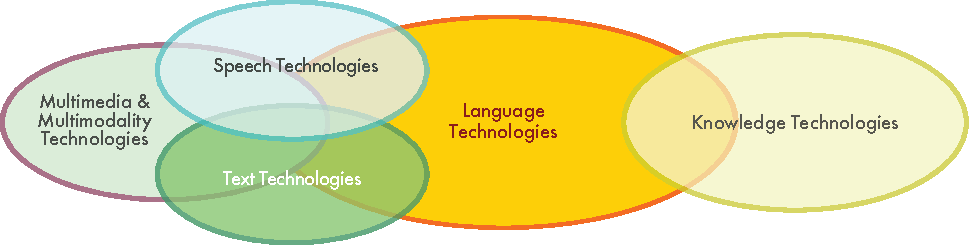
\includegraphics[width=\textwidth]{../_media/english/language_technologies}
  \caption{Language technology in context}
  \label{fig:ltincontext_en}
  \colorrule{grey3}{\textwidth}{1.5pt}
\end{figure*}

 When we communicate, we combine language with other modes of communication and information media – for example speaking can involve gestures and facial expressions. Digital text can contain pictures, charts, sounds, movies, etc. Movies can contain language in spoken and written form. In other words, speech and text technologies overlap and interact with other technologies that facilitate processing of multimodal communication and multimedia documents.

In the rest of this section, we first describe the architecture of a typical LT system. After that, we provide an overview of the core application areas, followed by a brief overview of the situation in LT research and education. Finally, the table at the end of the section summarizes an expert assessment of the situation regarding the core LT tools and resources in a number of dimensions such as availability, maturity, or quality.

\begin{figure*}[b]
  \colorrule{grey3}{\textwidth}{1.5pt}
  \center
  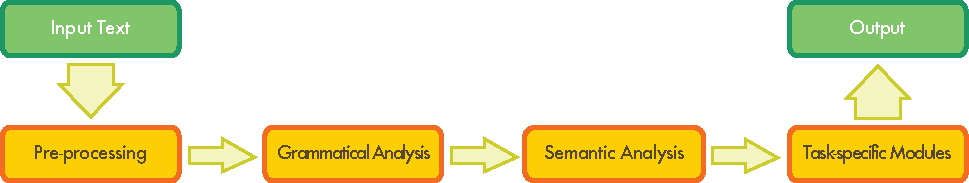
\includegraphics[width=\textwidth]{../_media/english/text_processing_app_architecture}
  \caption{A typical text processing architecture}
  \label{fig:textprocessingarch_en}
  \colorrule{grey3}{\textwidth}{1.5pt}
\end{figure*}


\subsection{Application Architectures}

Software applications for language processing typically consist of several components that mirror different aspects of language and of the task they implement. The figure on the right displays a highly simplified architecture that can be found in a text processing system. The first three modules deal with the structure and meaning of the text input:
\begin{enumerate}
  \item Pre-processing: cleaning up the data, removing formatting, detecting the input language, etc.
  \item Grammatical analysis: finding verb, its objects, modifiers and other sentence elements; analyzing the sentence structure.
  \item Semantic analysis: disambiguation (Which meaning of “apple” is the right one in the given context?), resolving coreferential expressions like “she”, “the car”, etc.; representing the meaning of the sentence in a machine-readable way
\end{enumerate}
Task-specific modules then perform many different operations such as automatic summarization of an input text, database look-ups and many others.
  
\subsection{Core Application Areas}

In the following, we will discuss the main application areas of language technology, i.e., language checking, web search, speech interaction, and machine translation. This includes applications and basic technologies such as
\begin{itemize}
  \item spelling correction
  \item authoring support
  \item computer-assisted language learning
  \item information retrieval
  \item information extraction
  \item text summarization
  \item question answering
  \item speech recognition
  \item speech synthesis
\end{itemize}
Below, we illustrate core application areas and highlight certain modules of the different architectures in each section. For expository reasons, the architectures are highly simplified and idealized.

\subsubsection{Language Checking}

  \begin{figure*}[t]
  \colorrule{grey3}{\textwidth}{1.5pt}
  \center
  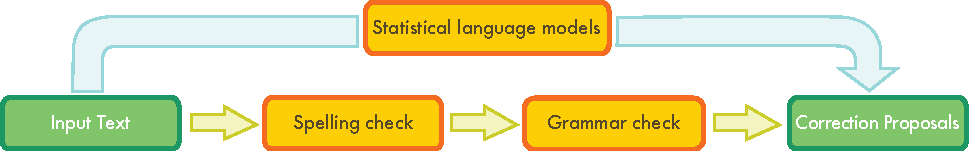
\includegraphics[width=\textwidth]{../_media/english/language_checking}
  \caption{Language checking (top: statistical; bottom: rule-based)}
  \label{fig:langcheckingaarch_en}
  \colorrule{grey3}{\textwidth}{1.5pt}
\end{figure*}

The morphological and syntactic properties of Czech constitute a great challenge for both spelling and grammar checking. Although the corresponding tools already exist for both kinds of checking (first spelling checkers date back to early 1990’s, the development of a first grammar checker for Microsoft Office took much longer time, it has been included as late as in 2005), there are still many issues waiting for an efficient solution.

The existing spelling checkers for Czech are based on a dictionary of basic word forms (lemmas) combined with a set of morphological rules enabling the analysis or generation of all correct word forms. Although this simple approach seems to be satisfactory, it has two substantial drawbacks. The first issue concerns the spelling errors which are actually correct word forms appearing in a wrong context. Due to the isolated handling of individual word forms it is virtually impossible to discover such errors; some more advanced error detection algorithms would definitely be useful. The second drawback is the inability to distinguish between real spelling errors and word forms which are correct, but which are missing from the dictionary. Such words will always exist due to the natural enhancement of a lexicon by newly created words, by new scientific or technical terms etc. The ability to capture this distinction would bring the spelling checkers to a new level.

Some attempts to make the spelling checking more context sensitive have already been made in the past. For example, one of the most frequent errors is incorrect spelling of personal pronoun \textit{já {[}I{]}} in the genitive, dative, accusative and locative cases. While the forms differ in spelling (\textit{mě} in genitive/accusative and \textit{mně} in dative/locative) their pronounciation is the same. Therefore,  many people write them incorrectly. To determine the correct form automatically theoretically requires a complete analysis of the given sentence because the proper case usually cannot be determined without taking into account syntax and/or verbal valency. This makes a development of a sophisticated grammar checker a challenge.

The solution implemented in Microsoft Word exploits the fact that these pronouns almost exclusively directly follow a preposition. If this preposition requires using only a particular case (like, e.g., the preposition \textit{k {[}to{]}}), then the correct pronominal form can be determined with almost 100\% reliability just on the basis of this local context. The Autocorrect tool of MS Word thus contains a simple list of such prepositions together with the correct pronominal form.

This example demonstrates that a further research of similar morphological or syntactic properties may improve the quality of a contextual spelling checker quite substantially.

Czech proves to be even more difficult for grammar checking than it is for spelling checking. As a language with a great degree of word-order freedom it makes it difficult to apply error pattern checking, a standard method used for languages with stricter word-order like English. The order of words in a Czech sentence is not completely arbitrary (for example, Czech clitics usually occupy a fixed position in the sentence), but in some cases it is even possible to tear apart an adjective from a nominal group and put it almost anywhere in a given sentence, like, e.g., in frequently cited examples \textit{Vánoční nadešel čas {[}Christmas(adj.) came time / A Christmas time has arrived{]}} or \textit{Hrdliččin zval ku lásce hlas {[}The turtle-dove‘s called to love voice / To love called the turtle-dove’s voice{]}}. Such discontinuous constructions, or non-projective constructions, constitute a huge challenge for any grammar checker. The investigation of the Prague Dependency Treebank, a syntactically annotated corpus of Czech, shows that about 14\% of sentences in the corpus contain at least one non-projective construction. This number clearly demonstrates that this phenomenon cannot be ignored.

These constructions make the grammar checking even more difficult for one more reason. The fact that a dependent word may be located very far from its governor also blurs the distinction between correct and incorrect sentences. Let us demonstrate this fact by means of the following example:

\textit{Které děvčata chtěla dostat šaty?\\
{[}Which girls wanted to\_get dresses?{]}}

This sentence may either be understood as a syntactically correct, but non-projective sentence which can be translated as \textit{Which dresses did the girls want to get?} or as a syntactically incorrect, but projective sentence \textit{Which girls wanted to get dresses?} (This reading is syntactically incorrect because of the wrong form of the interrogative pronoun \textit{Které {[}Which{]}} – the proper form being \textit{Která}.) To resolve this ambiguity is virtually impossible – non-projective constructions are an integral part of the Czech language and their presence in a sentence does not indicate anything unusual.

The syntactic complexity of non-projective constructions in Czech is even higher than the previous example may suggest. A simple Czech sentence may contain more than one such construction, as, e.g. the sentence:

\textit{Tuto knihu jsem se mu rozhodl dát k narozeninám.\\
{[}Lit.: This book I\_am myself to him decided to\_give to birthday.{]}\\
{[}I decided to give him this book to his birthday.{]}}

The pattern present in this example, namely the combination of a finite and infinite verb with intertwined dependent constituents, is very productive in Czech and it theoretically allows for an unlimited number of non-projective constructions in a single clause.

Although non-projective constructions constitute a great challenge for grammar checking because they make simple error-pattern based methods insufficient, they are not the only syntactic challenge in Czech. At least equally important seems to be another syntactic property of Czech – its ability to drop a subject of a subsequent sentence if it is clear from the context what the subject would be. Let us present yet another example:

\textit{Sportovci házely plyšáky.\\
{[}Sportsmen were throwing cuddle-bears.{]}}

This sentence is syntactically incorrect in the most typical reading due to a gender disagreement between the subject (\textit{sportovci} – masc. anim.) and the predicate (\textit{házely} – fem. or masc. inanimate). The situation changes, if we change the context in the following way:

\textit{Dívky křičely. Sportovci házely plyšáky a rozhodčím shnilá rajčata.\\
{[}Girls shouted. They were throwing cuddle-bears to the sportsman and rotten tomatoes to referees.{]}}

The fact that the subject may be omitted from a sentence makes it extremely difficult for existing grammar checkers of Czech to discover one of the most frequent types of grammatical errors, the errors in subject – predicate agreement. Further improvement may be achieved only if context broader than a single sentence is involved. This constitutes a great challenge for further research.

Although the first generation of spelling and grammar checkers for Czech already exist, other language checking tools do not. For example, in the field of authoring support we face a total lack of tools. This is caused to a certain extent by the fact that Czech is usually a target language for technical documentation of various products, not a source one, and thus the need for authoring tools is not as pressing as it is the case with more widely used languages. Nevertheless, the need for such tools will definitely grow in the future and thus the research in the natural language processing tools in this area will be more important.

\subsubsection{Web Search}

\begin{figure*}[htb]
  \colorrule{grey3}{\textwidth}{1.5pt}
  \center
  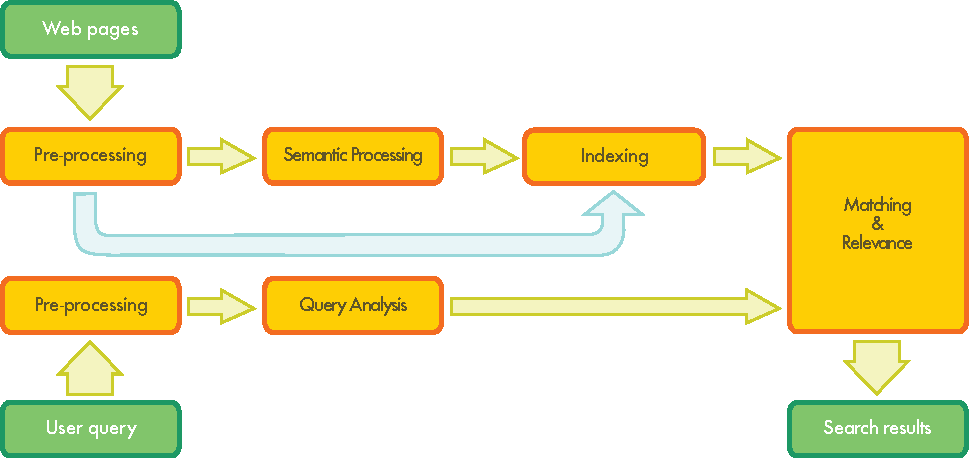
\includegraphics[width=\textwidth]{../_media/english/web_search_architecture}
  \caption{Web search}
  \label{fig:websearcharch_en}
  \colorrule{grey3}{\textwidth}{1.5pt}
 \end{figure*}

In the Czech Republic, there is a long tradition of using local web search engines. The most widely used web search engines are Seznam.cz, Google.com, Morfeo.cz and Jyxo.cz. Therefore, the situation is rather different from other countries, where Google.com has an 80\% majority. In the local market, there is enough room both for improving existing search engines through academia-industry collaboration, and for introducing a new one (especially if it would be restricted on a specific domain or specific task, e.g. question answering).

To the best of our knowledge, Google's results are considered to be the most relevant. Google started in 1998 and neither the search interface nor the presentation of the retrieved results has significantly changed since the first version. The success story of Google shows that with a lot of data at hand and efficient techniques for indexing these data, a mainly statistically-based approach can lead to satisfactory results.

However, for a more sophisticated information need, integrating deeper linguistic knowledge is essential. In particular, if a search query consists of a question or a complete sentence rather than a list of keywords, retrieving relevant answers to this query requires an analysis of this question or sentence on a syntactic and semantic level as well as the availability of an index that allows for a fast retrieval of relevant documents.

For example, imagine a user inputs the query “Give me a list of all companies that were taken over by other companies in the last five years”. A simple keyword-based approach will not take us very far here. Expanding the query terms by synonyms, for example using an ontological language resource like WordNet, may improve the results. However, for a satisfactory answer, a deeper query analysis is necessary. For example, applying a syntactic parser to analyze the grammatical structure of the sentence, we can determine that the user is looking for companies that have been taken over and not companies that took over others. We also need to process the expression “last five years” to find out which years it refers to.

For Czech, the sentence analysis task is rather complicated, because we must deal (as already mentioned) with rich morphology and free word order. The local search engines have already incorporated some kinds of morphological analyses into their systems, but their quality varies.

Finally, the processed query needs to be matched to a massive amount of unstructured data in order to find the piece or pieces of information the user is looking for. This involves the retrieval and ranking of relevant documents. In addition, generating a list of companies, we also need to extract the information that a particular string of words in a document refers to a company name. This kind of information is tagged using a named-entity recognizer.

We face an additional challenge if we want to match a query to documents written in a different language. For multilingual search, we have to automatically translate the query to all possible source languages and map the retrieved information back to the target language. Again, this requires a linguistic analysis of all texts involved. For users with a very specialized information need, an expansion of the query may require additional knowledge resources like a domain-specific ontology, representing the concepts relevant within the domain and the relationships between those concepts.

The increasing share of data available in non-textual format also drives the demand for services enabling multimedia search, i.e. information search on images, audio and video data. For audio and video files, this involves a \textbf{speech recognition} module to convert speech content into text or a phonetic representation, to which user queries can be matched.  
  
\subsubsection{Speech Technology}

General recognition of spoken Czech is still in its infancy. Simple applications that work with a small vocabulary and grammar have a high reliability, because Czech does not have a complex sound system. The main problems of applications with large vocabularies and more general language models is the large number of inflection forms of words, a relatively free word order and an informal Common Czech. This prevents statistical language modelling methods to achieve results similar to English.

 \begin{figure*}[htb]
  \colorrule{grey3}{\textwidth}{1.5pt}
  \center
  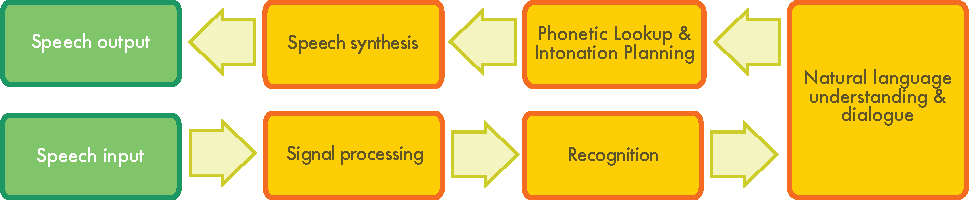
\includegraphics[width=\textwidth]{../_media/english/simple_speech-based_dialogue_architecture}
  \caption{Speech-based dialogue system}
  \label{fig:dialoguearch_en}
  \colorrule{grey3}{\textwidth}{1.5pt}
\end{figure*}

There are several commercial systems with large vocabularies available (SpeechTech s.r.o.\cite{Note11}, OptimSys, s.r.o.\cite{Note12}, NewtonTechnologies, a.s.\cite{Note13}), but they only work in dictation systems with a high quality audio input or very limited language domains like sporting events or parliamentary speeches. It is possible to buy a separate recognition engine with an open Media Resource Control Protocol  interface that allows the involvement of the recognition module into other applications. Companies offer applications generating off-line transcripts of multimedia archives allowing search. All these products have a relatively good configuration option, but they are not open source applications. For development of an open source recognizer of Czech, there is a lack of freely available acoustic training data, which would allow the preparation of free acoustic models for a speaker independent recognizer. Universal open source tools and libraries are available for the speech recognition, but a reliable method is still missing for the recognition of spontaneous Czech speech with all its word forms and free word order.
Czech \textbf{speech synthesis} has several commercial voices on a good quality level (Eris\cite{Note11}, Acapela Group\cite{Note14}), there are even open-source Czech synthetic voices, but with lower quality (Festival Czech\cite{Note15}, Epos TTS System\cite{Note16}, MBROLA\cite{Note17}). The speech synthesis modules are embeddable into Interactive Voice Response systems that support many open standards. To create more open source voices we are again missing open source audio recordings, which would allow the development of freely available high-quality voices.

Relying on the two technologies mentioned above, dialog systems are also in their developmental infancy. Czech dialog systems without restrictions are the goal of cooperative research of several universities. Some of speech departments are working on many projects in the speech field, being able to offer simple dialog systems, covering most of voice technology.

Research on spoken Czech focuses on improving the language model. In addition to the proven method of increasing the amount of language model training data, which requires time-consuming manual transcriptions, specific procedures are explored for the Czech language.

One line of research concentrates on conversion of spoken Czech to the formal written form, which can be processed by existing methods developed on \textbf{text corpora}.

Apart from simple cases of replacement of suffixes of Common Czech by their literary form, the method needs to address the replacement of whole word phrases by their correct form. Eliminated in a similar manner are the other phenomena of spontaneous speech such as filler words, repairs or listener responses.

The second line of research focuses on the development of syntactic and semantic analysers of Czech with the help of manually annotated tree corpora of written and spoken Czech. In conjunction with a morphological analysis, this method should help address problems of free word order and of the large number of word forms.

Current research on synthesized spoken Czech tries to develop more natural voices. Hopes are placed in advanced syntactic and semantic analysis of input texts, which should significantly improve the naturalness of utterances.

\subsubsection{Machine Translation}

The idea of using digital computers to translate natural languages can be traced back to 1946 and was followed by substantial funding for research during the 1950s and again in the 1980s. Yet \textbf{machine translation} (MT) still cannot deliver on its initial promise of providing across-the-board automated translation.

\boxtext{At its basic level, Machine Translation simply substitutes words in one natural language with words in another language.}
The idea of the translation by the computers became attractive for linguists and mathematicians in the Czech Republic very soon after the first experiments with MT in the world (1954 in USA, 1955 in Soviet Union). In January 1960 the first experiment with English-Czech MT of several sentences by the computer of the 1st generation SAPO, made in earlier Czechoslovakia, was carried out due to the efforts of the small research group from Charles University and the Research Institute of Mathematical Machines. The development of the methods used in MT was continuously followed by the university linguistic research group and some experimental rule-based systems of English-Czech and Czech-Russian MT systems were developed for the computers of 2nd generation (made in GDR and in USSR). They were domain-restricted and served mainly for a verification of formally expressed grammatical rules. In the 1990s a prototype of MT between closely related languages was proposed for the pair Czech and Slovak at Charles University (Česílko\cite{Note18}); however, its application fails due to practical reasons (such as high costs connected with its maintenance etc.). The strategy of statistical methods or combination of statistical and rule-based methods was chosen as a more prospective one for the future.
The most basic approach to machine translation is the automatic replacement of the words in a text written in one natural language with the equivalent words of another language. This can be useful in subject domains that have a very restricted, formulaic language such as weather reports (system METEO\cite{Note19}). However, in order to produce a good translation of less restricted texts, larger text units (phrases, sentences, or even whole passages) need to be matched to their closest counterparts in the target language. The major difficulty is that human language is ambiguous, which presents challenges on multiple levels, for example word sense disambiguation at the lexical level or the attachment of prepositional phrases on the syntactic level.

One way to build an MT system is to use linguistic rules. For translations between closely related languages, a translation using direct substitution may be feasible in cases such as the above example. However, rule-based (or linguistic knowledge-driven) systems often analyse the input text and create an intermediary symbolic representation from which the target language text can be generated. The success of these methods is highly dependent on the availability of extensive lexicons with morphological, syntactic, and semantic information, and large sets of grammar rules carefully designed by skilled linguists. This is a very long and therefore costly process.

\begin{figure*}[htb]
  \colorrule{grey3}{\textwidth}{1.5pt}
  \center
  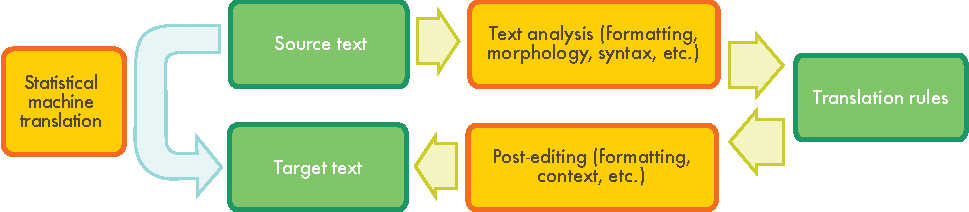
\includegraphics[width=\textwidth]{../_media/english/machine_translation}
  \caption{Machine translation (left: statistical; right: rule-based)}
  \label{fig:mtarch_en}
  \colorrule{grey3}{\textwidth}{1.5pt}
\end{figure*}

For Czech, there are several commercial and academic rule- and lexicon-based translation systems. One of them is based on a linguistic theory elaborated in Prague since 1960s. The system follows the above mentioned analysis-transfer-synthesis scenario. Despite the linguistic adequacy of such approach, the system still suffers from a number of practical difficulties, such as from relatively high error rate of current syntactic analysers and from computational issues related to high number of contextual features that should be taken into account when translating individual words.
In the late 1980s when computational power increased and became cheaper, interest in statistical models for machine translation began to grow. Statistical models are derived from analysing bilingual text corpora, \textbf{parallel corpora}, such as the Europarl parallel corpus, which contains the proceedings of the European Parliament in 21 European languages (Czech has been added recently and the size of Czech data is still orders of magnitude smaller than for established languages.) Given enough data, statistical MT works well enough to derive an approximate meaning of a foreign language text by processing parallel versions and finding plausible patterns of words. Unlike knowledge-driven systems, however, statistical (or data-driven) MT systems often generate ungrammatical output. Data-driven MT is advantageous because less human effort is required, and it can also cover special particularities of the language (e.\,g., idiomatic expressions) that are often ignored in knowledge-driven systems. 
Availability of large amounts of bilingual texts is really the key in statistical MT. For Czech, corpora of parallel texts with several other languages are currently being created. The largest data – in total several million pairs of sentences – is available for the English-Czech language pair\cite{Note20}. The corpus contains for example EU law texts, newspaper texts, technical documentation, and electronic books. The most challenging problem related to the contemporary parallel corpora is the quality of alignment (pairing of corresponding parts of a text and its translation). Not only that exact word-to-word linkage is impossible due to differences in morphology and syntax of the two languages, but reliable sentence-to-sentence and sometimes even document-to-document alignment is difficult to achieve too. Needless to say that compilation of such corpora has to be fully automatic – human processing is completely out of question because of the data size.

Languages with rich morphology like Czech also pose specific challenges for state-of-the-art statistical systems: the system has to choose not only the correct word but also the appropriate form to satisfy grammatical context. Very few statistical systems to date can handle morphological richness explicitly and thus often fall short of vocabulary: all the necessary word forms are not available even in large parallel corpora.
The strengths and weaknesses of knowledge-driven and data-driven machine translation tend to be complementary, so that nowadays researchers focus on hybrid approaches that combine both methodologies. One such approach uses both knowledge-driven and data-driven systems, together with a selection module that decides on the best output for each sentence. However, results for sentences longer than, say, 12 words, will often be far from perfect. A more effective solution is to combine the best parts of each sentence from multiple outputs; this can be fairly complex, as corresponding parts of multiple alternatives are not always obvious and need to be aligned. Another, more challenging approach is to design a new setup that combines the advantages of the two paradigms by integrating the good features of each. For example, making a rule-based system adaptive by adding a module for rule learning, or, making a statistical MT system syntax-aware by adding syntactical constraints.

Completely separate is the question of evaluating MT output quality, both manually and automatically. Experience shows that different systems score differently under various manual evaluations: rule-based systems tend to preserve the meaning better while statistical systems produce output more fluent locally. In e.g. question-answering evaluation, the meaning is more important. On the other hand, local fluency impacts the impression more when the user is directly comparing system outputs. Automatic evaluation (based on the comparison of MT output to one or more manually constructed reference translations) is vital in development of MT systems. It has been shown that such automatic evaluation is unreliable esp. for languages with richer morphology and it is also acknowledged that some automatic fine-grained reporting on MT quality and error types would be very useful.

\subsection{Information management/``LT behind the scenes''}

Building language technology applications involves a range of subtasks that do not always surface at the level of interaction with the user, but they provide significant service functionalities “behind the scenes” of the system in question. They all form important research issues that have now evolved into individual sub-disciplines of computational linguistics. Question answering, for example, is an active area of research for which annotated corpora have been built and scientific competitions have been initiated. The concept of question answering goes beyond keyword-based searches (in which the search engine responds by delivering a collection of potentially relevant documents) and enables users to ask a concrete question to which the system provides a single answer. For example:

\begin{itemize}
\item[] \textit{Question: How old was Neil Armstrong when he stepped on the moon?}
\item[] \textit{Answer: 38.}
\end{itemize}

While question answering is obviously related to the core area of web search, it is nowadays an umbrella term for such research issues as which different types of questions exist, and how they should be handled; how a set of documents that potentially contain the answer can be analysed and compared (do they provide conflicting answers?); and how specific information (the answer) can be reliably extracted from a document without ignoring the context. Question answering is in turn related to information extraction (IE), an area that was extremely popular and influential when computational linguistics took a statistical turn in the early 1990s. IE aims to identify specific pieces of information in specific classes of documents, such as the key players in company takeovers as reported in newspaper stories. Another common scenario that has been studied is reports on terrorist incidents. The task here consists of mapping appropriate parts of the text to a template that specifies the perpetrator, target, time, location and results of the incident. Domain-specific template-filling is the central characteristic of IE, which makes it another example of a “behind the scenes” technology that forms a well-demarcated research area, which in practice needs to be embedded into a suitable application environment.
\boxtext{Language technology applications often provide significant service functionalities behind the scenes of larger software systems.}
Text summarisation and \textbf{text generation} are two borderline areas that can act either as standalone applications or play a supporting role. Summarisation attempts to give the essentials of a long text in a short form, and is one of the features available in Microsoft Word. It mostly uses a statistical approach to identify the “important” words in a text (i.\,e., words that occur very frequently in the text in question but less frequently in general language use) and determine which sentences contain the most of these “important” words. These sentences are then extracted and put together to create the summary. In this very common commercial scenario, summarisation is simply a form of sentence extraction, and the text is reduced to a subset of its sentences. An alternative approach, for which some research has been carried out, is to generate brand new sentences that do not exist in the source text.
An alternative approach, to which some research is devoted, is to actually synthesize new sentences, i.e., to build a summary of sentences that need not show up in that form in the source text. This requires a certain amount of deeper understanding of the text and therefore is much less robust; furthermore, such an approach is to a good extent geared towards a particular domain or text genre, since particular knowledge is needed to perform the step of abstracting from the source text to its “content”. Synthesizing a summary now in turn is a case of text generation - the production of new text, either from other text (as in summarization), or from a set of non-textual data. This can be applied whenever reports are needed that describe how certain data streams develop over time. Such systems have been built for generating weather and air quality reports, or for summaries of medical diagnosis data. However, a text generator is in most cases not a stand-alone application but embedded into a larger software environment, such as into a clinical information system where patient data is collected, stored and processed, and report generation is just one of many functionalities.

There are many Czech research groups working on international (e.g. English) applications. Only a part of the HLT effort in the Czech Republic is dedicated particularly to Czech. There are many NLP-components for Czech, such as spell-checkers, corpora, morphological taggers and valency lexicons, along with a Czech collocation analyser (Word Sketch Engine for Czech, developed at the Masaryk University in Brno, (\cite{Horak2009})) and a manifold research of speech recognition and generation, but not many more complex HLT applications ready to use in the industry.

To the best of our knowledge, there is just one working question-answering system reported for Czech, developed by researchers at the Masaryk University in Brno – UIO (standing for the Czech “Artificial Intelligence of a Monkey”), (\cite{Svoboda2003}). UIO can ask databases and the Web. In its current version, UIO can be used for asking questions about train and coach timetables, cinema and theatre performances, about currency exchange rates, name-days and on the Diderot Encyclopedia. For all domains UIO has an accuracy rate about 80\%. A competing (so far no-name) system is being developed at the University of West Bohemia.

A simple conversational dialog system was developed at the Institute of Formal and Applied Linguistics, Charles University in Prague in collaboration with the Faculty of Cybernetics at the University of West Bohemia in Pilsen and, to a lesser extent, with some other consortium partners in the FP-6 Companions project\cite{Note21}. A human-like avatar converses with seniors about their respective personal photograph collections and life stories (\cite{Ptacek2010}, \cite{Romportl2010}, \cite{GruberTihelka2010}).

The Text-Mining Research Group at the University of West Bohemia is developing a User Profile Generation system (\cite{Grolmus2003}). This system performs text-mining on the documents gathered and viewed by a user. It uses the (user-approved) information to recommend particular documents on further searches as well as to estimate the user’s expertise in a given domain. This application can be used e.g. as a support of digital libraries.
WebGen, a similarly-named application developed at the Masaryk University in Brno (LSD lab\cite{Note22}) is a dialog-based system that helps visually impaired people generate web presentations in Czech. It is still in development (\cite{BartelPlhak2008}).

The Department of Computer Graphics and Multimedia FIT BUT Faculty of Information Technology at the Brno University of Technology in Brno\cite{Note23} delivered speech-processing software that adds semantic labels to speech transcripts (Speech Tagging, \cite{Smrz2010}). The client side is an HTML user interface in a web browser accessing functionality provided by the server. The server enables upload and analysis of speech records. The user is able to define and manage so called "tags", which are groups of semantically related keywords. If some keyword is found in some record, the record is tagged correspondingly. This service would be useful in e.g. crisis management, when it is suitable to classify phone calls according to words spoken, but, to our knowledge, it has not been employed in real applications yet.

The Faculty of Cybernetics at the University of West Bohemia in Pilsen has developed several speech-based applications for Czech, such as a dialog system with train timetables or a dialog system for students registering for exams on the phone (University VoiceXML information system\cite{Note24}). Their research groups run numerous projects aimed at assisting people with hearing impairments, e.g. by translating between Czech and (Czech) sign language.

Another useful application (developed in Pilsen) is a voice-controlled system for dentists (\cite{Nagy2008}). It works in two modes:  in the first, it reads the record of a tooth in the mouth of the patient. In the second mode, it records the information that the dentist dictates and updates the status of the given tooth. Voice-control is essential there, since the dentist is not allowed to touch either a screen or controls on a dictation device while examining the patient.

The research groups from the University of West Bohemia and from the Institute of Formal and Applied Linguistics at the Charles University in Prague participated in the international MALACH project (MALACH stands for “Multilingual Access to Large Spoken Archives” and means “messenger angel” in Hebrew), (\cite{Psutka2005}). They were in charge of speech recognition and semantic indexing of testimonies recorded in Czech and other Slavic languages. The Charles University now hosts one of the local access points to the archive of testimonies of holocaust survivors. (Other access points are located in the USA, Germany, Hungary, Izrael and Australia)

The nearly 52,000 videotaped testimonies of the Shoah Foundation Institute's Visual History Archive were recorded primarily between 1994 and 1999 in 56 countries and in 32 languages. While the majority of the interviews are with Jewish Holocaust survivors, the archive also includes the testimonies of political prisoners, Sinti and Roma (Gypsy) survivors, Jehovah's Witness survivors, survivors of eugenics policies, and homosexual survivors as well as rescuers and aid providers, liberators, and participants in war crimes trials.

The archive is accessible through an on-line interface, which enables the users browsing and viewing the testimonies, deploying an index of 55 thousand keywords and key phrases. The access point in Prague stores more than 500 testimonies in Czech, with average duration of 2 hours. Other testimonies have to be ordered online from the other access point, which usually takes a few hours.

\subsubsection{Miscellaneous}

It would be misleading to judge the NLP-HLT research of the respective countries only on the basis of how many resources and applications for their national language they have produced. In fact, there is a vicious circle in the NLP-HLT research for small languages: the grant agencies as well as the government want to support only the best teams. The best teams are the ones that produce the most internationally recognized publications. These are significantly easier to achieve in research that has international impact. While almost any improvement in any issue is interesting to report on big or strategic languages such as English, Chinese or Arabic, a research with the same outcome has a grossly humbler impact when reported on languages that are interesting only for their native speakers. To produce a good publication on a small language, a real breakthrough is needed, whereas, obviously, breakthroughs cannot be counted on to happen regularly.  Besides, even if a language-dependent result for a small language is considered a breakthrough by the local research community, it is still difficult to present to international reviewers who are not familiar with the language.
Also, language-independent solutions are generally preferred to the language-dependent ones, since their commercial application is cheaper. English is the natural first-choice language to experiment on in the European context, as there are comprehensive high-quality resources available for English. Also, the results are more easily compared within the international community.

As a consequence, national teams focus on English rather than relying on research on their national language. This is to be kept in mind when assessing the quality of national HLT/NLP research and development. A poor inventory of good HLT applications and resources for a small language does not necessarily imply poor research, but it can be a serious indicator of lacking governmental support policy. Targeted governmental support of national-language HLT is vital for language communities whose markets are too small for national-language HLT to be endorsed by the private sector.
 
\subsection{LT industry and programs}

Industrial deployment of language technologies is not widespread in Czechia. Businesses specialized in LT are rare. The same holds for research \& development departments of larger companies.

Web search engines and services (Seznam, Centrum, Google etc.) are nowadays generally capable of performing morphological analysis and lemmatization. Google offers phrase-based machine translation of websites and user-supplied text both to and from Czech. Seznam provides on-line dictionaries between Czech on one side and English, German, French, Italian, Spanish or Russian on the other side. However, they don’t provide translation of running text.

There are companies developing and publishing bilingual electronic dictionaries as Windows applications. These typically contain morphological analysis / lemmatization, some of them also a sort of ontology.

Cell phone manufacturers can use a Czech version of T9.

Office software packages (such as Microsoft Office 2010) provide Czech spellchecking, grammar checking, sometimes also machine translation and automatic speech recognition (voice input).

Phone switchboards and help/information applications employing automatic speech recognition are virtually unheard of. There have been pilot projects with ASR by university teams specialized in ASR (most notably the University of West Bohemia in Pilsen and the Technical University in Liberec) but there is no wide industrial application of such technologies.

Czech speech recognition was commercialized by Newton Technologies company—a spin-off of the Technical University in Liberec.

Most of the government-originating funding programs are maintained by the Czech Science Foundation (GAČR) and focused on basic research. Recently (2009), a new Technological Agency of the Czech Republic (Technologická agentura České republiky, TAČR) has been established, which shall focus on applied research. However, there are probably no LT-related projects funded by TAČR yet.

\subsection{LT research and education}

From the historical point of view, the terms ``computational linguistics'', ``natural language processing'' and ``speech recognition'' have been used for a longer time than the term language technologies, at least in the context of research and education. No matter the name, the disciplines related to natural language comprise a number of related subjects of research and education: theoretical linguistics, corpus linguistics, computer science, mathematics, machine learning etc.

Below, we list Czech institutes and departments focusing on research and education in computational linguistics and language processing. The list also provides information about their core research areas (CL – computational ling., CoL – corpus ling., TL – theoretical ling., ASR – automatic speech recognition) and what study programs they offer, if any.

\begin{enumerate}
\item Charles University in Prague
  \begin{itemize}
  \item Institute of Formal and Applied Linguistics (\textit{http://ufal.mff.cuni.cz}); CL, TL, ASR; BSc, MSc, PhD;
  \item Institute of Czech National Corpus (\textit{http://ucnk.ff.cuni.cz/english/index.php});CoL; PhD.
  \item Institute of Theoretical and Computational Linguistics (\textit{http://utkl.ff.cuni.cz}); CL; PhD;
  \end{itemize}
\item University of Economics in Prague
  \begin{itemize}
  \item Department of information and knowledge engineering (\textit{http://kizi5.vse.cz/});datamining, semantic web, ontologies; BSc, MSc, PhD;
  \end{itemize}
\item Czech Technical University in Prague
  \begin{itemize}
  \item Department of Cybernetics (\textit{http://cyber.felk.cvut.cz/}); robotics, artifitial   intelligence; BSc, MSc, PhD;
  \item Department of Circuit Theory (\textit{http://noel.feld.cvut.cz/speechlab/start.php?page=projects\&lang=en\#2});  ASR; BSc, MSc, PhD
  \end{itemize}
\item Masaryk University, Brno
  \begin{itemize}
  \item Natural Language Processing Centre (\textit{http://nlp.fi.muni.cz/en/nlplab}); CL, ASR; 
  \item Department of Czech Language (\textit{http://www.muni.cz/phil/211700?lang=en}); CL, TL;	BSc, MSc, PhD;
  \end{itemize}
\item Brno University of Technology
  \begin{itemize}
  \item Speech Processing Group (\textit{http://speech.fit.vutbr.cz/}); ASR; 
  \end{itemize}
  \begin{itemize}
  \item Natural Language Processing Research Group (\textit{http://www.fit.vutbr.cz/research/groups/nlp/index.php?lang=en}); CL; 
  \end{itemize}
\item University of West Bohemia
  \begin{itemize}
  \item Department of Cybernetics (\textit{http://www.kky.zcu.cz/en}); ASR; BSc, MSc, PhD;
  \end{itemize}
\item Technical University of Liberec
  \begin{itemize}
  \item Laboratory of Computer Speech Processing (\textit{https://www.ite.tul.cz/speechlabe/}); ASR; 
  \end{itemize}
\end{enumerate}

Charles University in Prague, Faculty of Mathematics and Physics is offering the European Master Program in Language and Communication Technologies as a part of its MSc. study program as well as PhD program. Thanks to this activity, the Faculty can welcome students from abroad who also give new impulses to their Czech colleagues.

The natural language research in the private sector is not very common in the Czech Republic and is only represented by small companies (e.g. Lingea, Captaworks, LangSoft) and by spin-offs of university teams (e.g. SpeechTech - University of West Bohemia, Phonexia - University of Technology in Brno).

The study programs the institutes offer emphase both theory and practice. Unfortunately, a demand for such experts is very low in the Czech Republic.

\subsection{Availability of tools and resources for Czech}
The following table summarizes the current state of language technology support for the Czech language. The rating for existing tools and resources is based on assessments of leading experts (0 is worst, 6 is best).

\begin{figure*}[htb]
\centering
\begin{tabular}{>{\columncolor{orange1}}p{.33\linewidth}@{\hspace*{6mm}}c@{\hspace*{6mm}}c@{\hspace*{6mm}}c@{\hspace*{6mm}}c@{\hspace*{6mm}}c@{\hspace*{6mm}}c@{\hspace*{6mm}}c}
\rowcolor{orange1}
 \cellcolor{white}&
 \begin{sideways}\makecell[l]{Quantity}\end{sideways} &
 \begin{sideways}\makecell[l]{\makecell[l]{Availability} }\end{sideways} &
 \begin{sideways}\makecell[l]{Quality}\end{sideways} &
 \begin{sideways}\makecell[l]{Coverage}\end{sideways} &
 \begin{sideways}\makecell[l]{Maturity}\end{sideways} &
 \begin{sideways}\makecell[l]{Sustainability}\end{sideways} &
 \begin{sideways}\makecell[l]{Adaptability}\end{sideways} \\ \addlinespace

\multicolumn{8}{>{\columncolor{orange2}}l}{\textcolor{black}{Language Technology: Tools, Technologies and Applications}} \\ \addlinespace

Speech Recognition		  & 3 & 4 & 4 & 3 & 3 & 4 & 3\\ \addlinespace
Speech Synthesis      & 3 & 3 & 3 & 4 & 3 & 3 & 2\\ \addlinespace
Grammatical analysis       & 4 & 2 & 4 & 4 & 3 & 2 & 4\\ \addlinespace
Semantic analysis        & 1 & 1 & 2 & 2 & 1 & 2 & 2\\ \addlinespace
Text generation         & 2 & 1 & 3 & 3 & 3 & 2 & 4\\ \addlinespace
Machine translation          & 4 & 3 & 1 & 2 & 3 & 2 & 3\\ \addlinespace

\multicolumn{8}{>{\columncolor{orange2}}l}{\textcolor{black}{Language Resources: Resources, Data and Knowledge Bases}} \\ \addlinespace

Text corpora           & 4 & 3 & 5 & 4 & 5 & 4 & 1\\ \addlinespace
Speech corpora      & 4 & 1 & 4 & 2 & 3 & 3 & 2\\ \addlinespace
Parallel corpora         & 2 & 4 & 2 & 3 & 2 & 2 & 3\\ \addlinespace
Lexical resources          & 4 & 2 & 3 & 4 & 2 & 3 & 2\\ \addlinespace
Grammars                 & 1 & 1 & 3 & 2 & 2 & 1 & 1\\ \addlinespace

\end{tabular}
\label{tab:lrlttable}
\caption{State of language technology support for Czech}
\end{figure*}

\subsubsection{Notes to the table}

\begin{itemize}
\item While some specific corpora of high quality exist, a very large syntactically annotated corpus is not available.
\item There is a highly elaborated syntactically annotated corpus for Czech. However, the corpus is not available for free (can be bought via LDC). Several extending annotations (coreference, discourse etc.) are being performed on top of the corpus, but they are not yet finished.
\item For Czech, a large text corpus exists, but it is not available for automatic processing (only for on-line searching).
\item Many of the resources lack standardization, i.e., even if they exist, sustainability is not given; concerted programs and initiatives are needed to standardize data and interchange formats.
\item Semantics is more difficult than syntax; text semantics is more difficult than word and sentence semantics.
\item Research has been successful in designing particular high quality software, but it is nearly impossible to come up with sustainable and standardized solutions given the current funding situations.
\item There is an ontological resource for Czech (even mapped to other European ontological resources) but its coverage is limited.
\item Speech Recognition of Czech is researched at several universities and workplaces but free tools and data are not available.
\item The main problems of large vocabulary speech recognizers are in specific Czech language modelling.
\item In the field of speech synthesis, there are available open-source packages, but the speech synthesis with more natural voices is available only in commercial applications.
\item Czech dialogue systems are very little used due to poor accessibility of high quality speech recognition modules of Czech.
\item For the web search, there is enough room both for improving existing popular local search engines through the academia-industry collaboration, and for introducing a new one.
\end{itemize}
To conclude, in a number of specific areas of Czech language research, we have software with limited functionality and resources with limited scope/complexity available today, and only some of them open-source. Obviously, further research efforts are required to meet the current deficits.

\subsection{Cross-language comparison}
    The current state of LT support varies considerably from one language community to another. In order to compare the situation between languages, this section will present an evaluation based on two sample application areas (\textbf{machine translation} and speech processing) and one underlying technology (text analysis), as well as basic resources needed for building LT applications.

The above tables show that LT resources and tools for Czech clearly do not yet reach the quality and coverage of comparable resources and tools for the English language and some other ‘larger’ languages in EU. And there are still plenty of gaps in English language resources with regard to high quality applications.

Today’s text analysis components and language resources cover the linguistic phenomena of Czech only to a certain extent; they mostly form part of applications involving shallow natural language processing, e.g. spelling correction.

However, for building more sophisticated applications, such as machine translation, there is a clear need for resources and technologies that cover a wider range of linguistic aspects and allow a deep \textbf{semantic analysis} of the input text. By improving the quality and coverage of these basic resources and technologies, we shall be able to open up new opportunities for tackling a vast range of advanced application areas, including high-quality broad-based machine translation.

\subsection{Conclusions}

\emph{In this series of white papers, we have made an important effort by assessing the language technology support for 30 European languages, and by providing a high-level comparison across these languages. By identifying the gaps, needs and deficits, the European language technology community and its related stakeholders are now in a position to design a large scale research and development programme aimed at building a truly multilingual, technology-enabled communication across Europe.}
The results of this white paper series show that there is a dramatic difference in language technology support between the various European languages. While there are good quality software and resources available for some languages and application areas, others, usually smaller languages, have substantial gaps. Many languages lack basic technologies for text analysis and the essential resources. Others have basic tools and resources but the implementation of for example semantic methods is still far away. Therefore a large-scale effort is needed to attain the ambitious goal of providing high-quality language technology support for all European languages, for example through high quality machine translation. 
In the case of the Czech language, we can be cautiously optimistic about the current state of language technology support. There is a viable LT research community in the Czech Republic, which has been supported in the past by various research programs. A number of resources and technologies have been produced for Czech. However, the scope of the resources and the range of tools are still very limited when compared to the resources and tools for the English language, and they are simply not sufficient in quality and quantity to develop the kind of technologies required to support a truly multilingual knowledge society.

Nor can we simply transfer technologies already developed and optimized for the English language to handle Czech. English-based systems for parsing (syntactic and \textbf{grammatical analysis} of sentence structure) typically perform far less well on Czech texts, due to the specific characteristics of the Czech language.

The Czech language technology industry dedicated to transforming research into products is currently fragmented and disorganized. Most large companies have either stopped or severely cut their LT efforts, leaving the field to a number of specialized SMEs that are not robust enough to address the internal and the global market with a sustained strategy. 

Our findings show that the only alternative is to make a substantial effort to create LT resources for Czech, and use them to drive forward research, innovation and development. The need for large amounts of data and the extreme complexity of language technology systems makes it vital to develop a new infrastructure and a more coherent research organization to spur greater sharing and cooperation.
Finally there is a lack of continuity in research and development funding. Short-term coordinated programmes tend to alternate with periods of sparse or zero funding. In addition, there is an overall lack of coordination with programmes in other EU countries and at the European Commission level.

The long term goal of META-NET is to enable the creation of high-quality language technology for all languages. This requires all stakeholders - in politics, research, business, and society - to unite their efforts. The resulting technology will help tear down existing barriers and build bridges between Europe’s languages, paving the way for political and economic unity through cultural diversity.
\end{multicols}

\clearpage

\begin{figure*}[t]
\small
\centering
\begin{tabular}
{ % defines color for each column.
>{\columncolor{corange5}} p{.17\linewidth}@{\hspace{.027\linewidth}}
>{\columncolor{corange4}}p{.17\linewidth}@{\hspace{.027\linewidth}}
>{\columncolor{corange3}}p{.17\linewidth}@{\hspace{.027\linewidth}}
>{\columncolor{corange2}}p{.17\linewidth}@{\hspace{.027\linewidth}}
>{\columncolor{corange1}}p{.17\linewidth} 
}
\rowcolor{orange1} % redefines color for all columns in row 1
\begin{center}\vspace*{-2mm}\textbf{Cluster 1}\end{center} & 
\begin{center}\vspace*{-2mm}\textbf{Cluster 2}\end{center} & 
\begin{center}\vspace*{-2mm}\textbf{Cluster 3}\end{center} & 
\begin{center}\vspace*{-2mm}\textbf{Cluster 4}\end{center} & 
\begin{center}\vspace*{-2mm}\textbf{Cluster 5}\end{center} \\ \addlinespace

& \vspace*{0.5mm}Angličtina
& \vspace*{0.5mm}
Čeština \newline 
Finština \newline 
Francouzština \newline 
Holandština \newline 
Italština \newline  
Němčina \newline   
Portugalština \newline 
Španělština \newline
& \vspace*{0.5mm}Baskičtina \newline 
Bulharština \newline 
Dánština \newline 
Estonština \newline 
Galicijština\newline 
Irština \newline  
Katalánština \newline 
Maďarština  \newline
Norština \newline 
Polština \newline 
Řečtina \newline  
Srbština \newline 
Slovenština \newline 
Slovinština \newline 
Švédština \newline
& \vspace*{0.5mm}
Chorvatština \newline 
Islandština \newline  
Litevština \newline 
Lotyština \newline 
Maltština \newline 
Rumunština\\
\end{tabular}
\label{fig:speech_cluster}
\caption{Jazykové skupiny pro zpracování mluvené řeči}
\end{figure*}

\begin{figure*}[b]
\small
\centering
\begin{tabular}
{ % defines color for each column.
>{\columncolor{corange5}} p{.17\linewidth}@{\hspace{.027\linewidth}}
>{\columncolor{corange4}}p{.17\linewidth}@{\hspace{.027\linewidth}}
>{\columncolor{corange3}}p{.17\linewidth}@{\hspace{.027\linewidth}}
>{\columncolor{corange2}}p{.17\linewidth}@{\hspace{.027\linewidth}}
>{\columncolor{corange1}}p{.17\linewidth} 
}
\rowcolor{orange1} % redefines color for all columns in row 1
\begin{center}\vspace*{-2mm}\textbf{Cluster 1}\end{center} & 
\begin{center}\vspace*{-2mm}\textbf{Cluster 2}\end{center} & 
\begin{center}\vspace*{-2mm}\textbf{Cluster 3}\end{center} & 
\begin{center}\vspace*{-2mm}\textbf{Cluster 4}\end{center} & 
\begin{center}\vspace*{-2mm}\textbf{Cluster 5}\end{center} \\ \addlinespace

& \vspace*{0.5mm} Angličtina 
& \vspace*{0.5mm} 
Francouzština \newline 
Španělština
& \vspace*{0.5mm}
Holandština \newline 
Italština \newline 
Katalánština \newline 
Maďarština \newline
Němčina \newline 
Polština \newline 
Rumunština \newline 
& \vspace*{0.5mm}Baskičtina \newline 
Bulharština \newline 
Chorvatština \newline 
Čeština \newline
Dánština \newline 
Estonština \newline 
Finština \newline 
Galicijština \newline 
Islandština \newline 
Irština \newline 
Litevština \newline 
Lotyština \newline 
Maltština \newline 
Norština \newline 
Portugalština \newline 
Řečtina \newline 
Srbština \newline 
Slovenština \newline 
Slovinština \newline 
Švédština \newline 
\end{tabular}
\label{fig:mt_cluster}
\caption{Jazykové skupiny pro strojový překlad}
\end{figure*}

\begin{figure*}[t]
  \small
  \centering
  \begin{tabular}
{ % defines color for each column.
>{\columncolor{corange5}} p{.17\linewidth}@{\hspace{.027\linewidth}}
>{\columncolor{corange3}}p{.17\linewidth}@{\hspace{.027\linewidth}}
>{\columncolor{corange3}}p{.17\linewidth}@{\hspace{.027\linewidth}}
>{\columncolor{corange2}}p{.17\linewidth}@{\hspace{.027\linewidth}}
>{\columncolor{corange1}}p{.17\linewidth} 
}
\rowcolor{orange1} % redefines color for all columns in row 1
\begin{center}\vspace*{-2mm}\textbf{Cluster 1}\end{center} & 
\begin{center}\vspace*{-2mm}\textbf{Cluster 2}\end{center} & 
\begin{center}\vspace*{-2mm}\textbf{Cluster 3}\end{center} & 
\begin{center}\vspace*{-2mm}\textbf{Cluster 4}\end{center} & 
\begin{center}\vspace*{-2mm}\textbf{Cluster 5}\end{center} \\ \addlinespace

& \vspace*{0.5mm}Angličtina
& \vspace*{0.5mm}
  Francouzština \newline 
  Holandština \newline 
  Italština \newline 
  Němčina \newline 
  Španělština
& \vspace*{0.5mm}Baskičtina \newline 
  Bulharština \newline 
  Čeština \newline 
  Dánština \newline 
  Finština \newline 
  Galicijština \newline 
  Katalánština \newline 
  Maďarština \newline 
  Norština \newline 
  Polština \newline 
  Portugalština \newline 
  Rumunština \newline 
  Řečtina \newline 
  Slovenština \newline 
  Slovinština \newline 
  Švédština \newline 
& \vspace*{0.5mm}
  Chorvatština \newline 
  Estonština \newline 
  Irština \newline 
  Islandština \newline 
  Litevština \newline 
  Lotyština \newline 
  Maltština \newline 
  Srbština \\
  \end{tabular}
\label{fig:text_cluster}
\caption{Jazykové skupiny pro analýzu textu}
\end{figure*}

\begin{figure*}[b]
  \small
  \centering
\begin{tabular}
{ % defines color for each column.
>{\columncolor{corange5}} p{.17\linewidth}@{\hspace{.027\linewidth}}
>{\columncolor{corange4}}p{.17\linewidth}@{\hspace{.027\linewidth}}
>{\columncolor{corange3}}p{.17\linewidth}@{\hspace{.027\linewidth}}
>{\columncolor{corange2}}p{.17\linewidth}@{\hspace{.027\linewidth}}
>{\columncolor{corange1}}p{.17\linewidth} 
}
\rowcolor{orange1} % redefines color for all columns in row 1
\begin{center}\vspace*{-2mm}\textbf{Cluster 1}\end{center} & 
\begin{center}\vspace*{-2mm}\textbf{Cluster 2}\end{center} & 
\begin{center}\vspace*{-2mm}\textbf{Cluster 3}\end{center} & 
\begin{center}\vspace*{-2mm}\textbf{Cluster 4}\end{center} & 
\begin{center}\vspace*{-2mm}\textbf{Cluster 5}\end{center} \\ \addlinespace
    
& \vspace*{0.5mm}Angličtina
& \vspace*{0.5mm} 
    Čeština \newline 
    Francouzština \newline 
    Holandština \newline 
    Italština \newline
    Maďarština \newline
    Němčina \newline 
    Polština \newline
    Španělština \newline
    Švédština \newline 
& \vspace*{0.5mm} Baskičtina\newline 
    Bulharština\newline 
    Chorvatština \newline 
    Dánština \newline 
    Estonština \newline 
    Finština \newline 
    Galicijština \newline 
    Katalánština \newline 
    Norština \newline 
    Portugalština \newline 
    Rumunština \newline 
    Řečtina \newline 
    Srbština \newline 
    Slovenština \newline 
    Slovinština \newline
&  \vspace*{0.5mm}
    Irština \newline 
    Islandština \newline 
    Litevština \newline 
    Lotyština \newline 
    Maltština  \\
  \end{tabular}
  \label{fig:resources_cluster}
  \caption{Jazykové skupiny pro jazykové zdroje}
\end{figure*}


\clearpage
%-----------------------------------------

\ssection[About META-NET]{About META-NET}
\begin{multicols}{2}
META-NET is a Network of Excellence funded by the European Commission. The network currently consists of 54 members from 33 European countries \cite{rehm2011}. META-NET fosters the Multilingual Europe Technology Alliance (META), a growing community of language technology professionals and organisations in Europe. META-NET cooperates with other initiatives like the Common Language Resources and Technology Infrastructure (CLARIN), which is helping to establish digital humanities research in Europe. META-NET fosters the technological foundations for a truly multilingual European information society that:

\begin{itemize}
\item makes communication and cooperation possible across languages;
\item provides equal access to information and knowledge in any language;
\item offers advanced and affordable networked information technology to European citizens.
\end{itemize}

META-NET stimulates and promotes multilingual technologies for all European languages. The technologies enable automatic translation, content production, information processing and knowledge management for a wide variety of applications and subject domains. The network wants to improve current approaches, so better communication and cooperation across languages can take place. Europeans have an equal right to information and knowledge regardless of language.

META-NET launched on 1 February 2010 with the goal of advancing research in language technology (LT). The network supports a Europe that unites as a single digital market and information space. META-NET has conducted several activities that further its goals. META-VISION, META-SHARE and META-RESEARCH are the network’s three lines of action.

\textbf{META-VISION} fosters a dynamic and influential stakeholder community that unites around a shared vision and a common strategic research agenda (SRA). The main focus of this activity is to build a coherent and cohesive LT community in Europe by bringing together representatives from highly fragmented and diverse groups of stakeholders. In the first year of META-NET, presentations at the FLaReNet Forum (Spain), Language Technology Days (Luxembourg), JIAMCATT 2010 (Luxembourg), LREC 2010 (Malta), EAMT 2010 (France) and ICT 2010 (Belgium) centred on public outreach. According to initial estimates, META-NET has already contacted more than 2,500 LT professionals to develop its goals and visions with them. At the META-FORUM 2010 event in Brussels, META-NET communicated the initial results of its vision building process to more than 250 participants. In a series of interactive sessions, the participants provided feedback on the visions presented by the network. 

\textbf{META-SHARE} creates an open, distributed facility for exchanging and sharing resources. The peer-to-peer network of repositories will contain language data, tools and web services that are documented with high-quality metadata and organised in standardised categories. The resources can be readily accessed and uniformly searched. The available resources include free, open source materials as well as restricted, commercially available, fee-based items. META-SHARE targets existing language data, tools and systems as well as new and emerging products that are required for building and evaluating new technologies, products and services. The reuse, combination, repurposing and re-engineering of language data and tools plays a crucial role. META-SHARE will eventually become a critical part of the LT marketplace for developers, localisation experts, researchers, translators and language professionals from small, mid-sized and large enterprises. META-SHARE addresses the full development cycle of LT—from research to innovative products and services. A key aspect of this activity is establishing META-SHARE as an important and valuable part of a European and global infrastructure for the LT community. 

\textbf{META-RESEARCH} builds bridges to related technology fields. This activity seeks to leverage advances in other fields and to capitalise on innovative research that can benefit language technology. In particular, this activity wants to bring more semantics into machine translation (MT), optimise the division of labour in hybrid MT, exploit context when computing automatic translations and prepare an empirical base for MT. META-RESEARCH is working with other fields and disciplines, such as machine learning and the Semantic Web community. META-RESEARCH focuses on collecting data, preparing data sets and organising language resources for evaluation purposes; compiling inventories of tools and methods; and organising workshops and training events for members of the community. This activity has already clearly identified aspects of MT where semantics can impact current best practices. In addition, the activity has created recommendations on how to approach the problem of integrating semantic information into MT. META-RESEARCH is also finalising a new language resource for MT, the Annotated Hybrid Sample MT Corpus, which provides data for English-German, English-Spanish and English-Czech language pairs. META-RESEARCH has also developed software that collects multilingual corpora that are hidden on the Web.
\end{multicols}


\vfill
\centerline{office@meta-net.eu -- http://www.meta-net.eu}

\cleardoublepage

\appendix
\addtocontents{toc}{\protect\bigskip}

\bsection[Literaturverweise -- References]{Literaturverweise --- References} % Please translate this into Czech
\bibliographystyle{unsrt}
\bibliography{czech_references}

\cleardoublepage



\bsection[META-NET Mitglieder -- META-NET Members]{META-NET Mitglieder --- META-NET Members} % Please translate this into Czech
\label{metanetmembers}

\small
\begin{longtable}{@{}llp{113mm}@{}}
  Rakousko & \textcolor{grey1}{Austria} & Zentrum für Translationswissenschaft, Universität Wien: Gerhard Budin\\ \addlinespace 
  Belgie & \textcolor{grey1}{Belgium} & Computational Linguistics and Psycholinguistics Research Centre, University of Antwerp: Walter Daelemans\\ \addlinespace
  & & Centre for Processing Speech and Images, University of Leuven: Dirk van Compernolle \\ \addlinespace
  Bulharsko & \textcolor{grey1}{Bulgaria} & Institute for Bulgarian Language, Bulgarian Academy of Sciences: Svetla Koeva \\ \addlinespace
  Chorvatsko & \textcolor{grey1}{Croatia} & Institute of Linguistics, Faculty of Humanities and Social Science, University of Zagreb: Marko Tadić \\ \addlinespace
  Kypr & \textcolor{grey1}{Cyprus} & Language Centre, School of Humanities: Jack Burston \\ \addlinespace
  Česká republika & \textcolor{grey1}{Czech Republic} & Institute of Formal and Applied Linguistics, Charles University in Prague: Jan Hajič \\ \addlinespace 
  Dánsko &  \textcolor{grey1}{Denmark} & Centre for Language Technology, University of Copenhagen: \newline Bolette Sandford Pedersen, Bente Maegaard\\ \addlinespace
  Estonsko & \textcolor{grey1}{Estonia} & Institute of Computer Science, University of Tartu: Tiit Roosmaa, Kadri Vider\\ \addlinespace
  Finsko & \textcolor{grey1}{Finland} & Computational Cognitive Systems Research Group, Aalto University: Timo Honkela\\ \addlinespace
  & & Department of Modern Languages, University of Helsinki: Kimmo Koskenniemi,\newline Krister Lindén \\ \addlinespace
  Francie & \textcolor{grey1}{France} & Centre National de la Recherche Scientifique, Laboratoire d'Informatique pour la Mécanique et les Sciences de l'Ingénieur and Institute for Multilingual and Multimedia Information: Joseph Mariani \\ \addlinespace
  & & Evaluations and Language Resources Distribution Agency: Khalid Choukri\\ \addlinespace
  Německo & \textcolor{grey1}{Germany} & Language Technology Lab, DFKI: Hans Uszkoreit, Georg Rehm\\ \addlinespace
  & & Human Language Technology and Pattern Recognition, RWTH Aachen University: Hermann Ney \\ \addlinespace
  & & Department of Computational Linguistics, Saarland University: Manfred Pinkal\\ \addlinespace 
  Řecko & \textcolor{grey1}{Greece} & R.C. “Athena”, Institute for Language and Speech Processing: Stelios Piperidis\\ \addlinespace
  Maďarsko & \textcolor{grey1}{Hungary} & Research Institute for Linguistics, Hungarian Academy of Sciences: Tamás Váradi\\  \addlinespace
  & & Department of Telecommunications and Media Informatics, Budapest University of Technology and Economics: Géza Németh, Gábor Olaszy\\ \addlinespace
  Island & \textcolor{grey1}{Iceland} & School of Humanities, University of Iceland: Eiríkur Rögnvaldsson\\ \addlinespace
  Irsko & \textcolor{grey1}{Ireland} & School of Computing, Dublin City University: Josef van Genabith\\ \addlinespace
  Itálie & \textcolor{grey1}{Italy} & Consiglio Nazionale delle Ricerche, Istituto di Linguistica Computazionale “Antonio Zampolli”: Nicoletta Calzolari\\ \addlinespace
  & & Human Language Technology Research Unit, Fondazione Bruno Kessler:\newline Bernardo Magnini\\ \addlinespace
  Lotyšsko & \textcolor{grey1}{Latvia} & Tilde: Andrejs Vasiļjevs\\ \addlinespace 
  & & Institute of Mathematics and Computer Science, University of Latvia: Inguna Skadiņa\\ \addlinespace
  Litva & \textcolor{grey1}{Lithuania} & Institute of the Lithuanian Language: Jolanta Zabarskaitė\\ \addlinespace
  Lucembursko & \textcolor{grey1}{Luxembourg} & Arax Ltd.: Vartkes Goetcherian\\ \addlinespace
  Malta & \textcolor{grey1}{Malta} & Department Intelligent Computer Systems, University of Malta: Mike Rosner\\ \addlinespace
  Nizozemí & \textcolor{grey1}{Netherlands} & Utrecht Institute of Linguistics, Utrecht University: Jan Odijk\\ \addlinespace 
  & & Computational Linguistics, University of Groningen: Gertjan van Noord\\ \addlinespace
  Norsko & \textcolor{grey1}{Norway} & Department of Linguistic, University of Bergen: Koenraad De Smedt\\ \addlinespace 
  & & Department of Informatics, Language Technology Group, University of Oslo:\newline Stephan Oepen \\ \addlinespace
  Polsko & \textcolor{grey1}{Poland} & Institute of Computer Science, Polish Academy of Sciences: Adam Przepiórkowski, Maciej Ogrodniczuk \\ \addlinespace
  & & University of Łódź: Barbara Lewandowska-Tomaszczyk, Piotr Pęzik\\ \addlinespace
  & & Department of Computer Linguistics and Artificial Intelligence, Adam Mickiewicz University: Zygmunt Vetulani \\ \addlinespace
  Portugalsko & \textcolor{grey1}{Portugal} & University of Lisbon: António Branco, Amália Mendes \\ \addlinespace
  & & Spoken Language Systems Laboratory, Institute for Systems Engineering and Computers: Isabel Trancoso \\ \addlinespace
  Rumunsko & \textcolor{grey1}{Romania} & Research Institute for Artificial Intelligence, Romanian Academy of Sciences:\newline Dan Tufiș \\ \addlinespace
  & & Faculty of Computer Science, University Alexandru Ioan Cuza of Iași: Dan Cristea \\ \addlinespace
  Srbsko & \textcolor{grey1}{Serbia} & University of Belgrade, Faculty of Mathematics: Duško Vitas, Cvetana Krstev,\newline Ivan Obradović \\ \addlinespace
  & & Pupin Institute: Sanja Vranes \\ \addlinespace
  Slovensko & \textcolor{grey1}{Slovakia} & Ľudovít Štúr Institute of Linguistics, Slovak Academy of Sciences: Radovan Garabík \\ \addlinespace 
  Slovinsko & \textcolor{grey1}{Slovenia} & Jožef Stefan Institute: Marko Grobelnik \\ \addlinespace 
  Španělsko & \textcolor{grey1}{Spain} & Barcelona Media: Toni Badia, Maite Melero \\ \addlinespace 
  & & Institut Universitari de Lingüística Aplicada, Universitat Pompeu Fabra: Núria Bel \\ \addlinespace 
  & & Aholab Signal Processing Laboratory, University of the Basque Country:\newline Inma Hernaez Rioja \\ \addlinespace 
  & & Center for Language and Speech Technologies and Applications, Universitat Politècnica de Catalunya:  Asunción Moreno \\ \addlinespace 
  & & Department of Signal Processing and Communications, University of Vigo:\newline Carmen García Mateo \\ \addlinespace
  Švédsko & \textcolor{grey1}{Sweden} & Department of Swedish, University of Gothenburg: Lars Borin \\ \addlinespace 
  UK & \textcolor{grey1}{UK} & 
  School of Computer Science, University of Manchester: Sophia Ananiadou \\ \addlinespace 
  & & Institute for Language, Cognition and Computation, Center for Speech Technology Research, University of Edinburgh: Steve Renals \\ \addlinespace 
  & & Research Institute of Informatics and Language Processing, University of Wolverhampton: Ruslan Mitkov \\ \addlinespace  
  Schweiz & \textcolor{grey1}{Switzerland} & Idiap Research Institute: Hervé Bourlard  % Please translate this into Czech
    
\end{longtable}
\normalsize
 
\renewcommand*{\figureformat}{}
\renewcommand*{\captionformat}{}

\begin{figure*}[htbp]
  \colorrule{grey3}{\textwidth}{1.5pt}
  \center
  %\fbox{-- META-NET group picture omitted to keep the size of the PDF file small. --}
  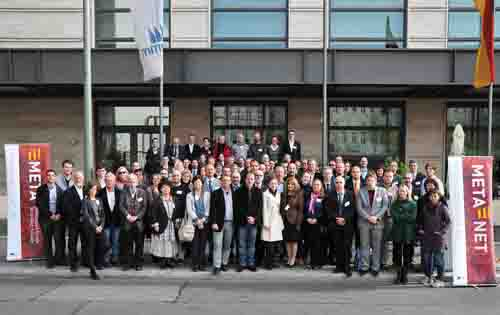
\includegraphics[width=\textwidth]{../_media/meta-net_team.jpg}
  \caption{Etwa 100 Experten des Gebiets Sprachtechnologie -- Repräsentanten der in META-NET vertretenen Länder und Sprachen -- diskutierten und finalisierten die zentralen Ergebnisse der Weißbuch-Serie bei einem META-NET-Treffen in Berlin am 21./22.~Oktober 2011. --- \textcolor{grey1}{About 100 language technology experts -- representatives of the countries and languages represented in META-NET -- discussed and finalised the key results and messages of the White Paper Series at a META-NET meeting in Berlin, Germany, on October 21/22, 2011.}}
  \medskip
  \colorrule{grey3}{\textwidth}{1.5pt}
\end{figure*}

\cleardoublepage

\bsection[Série Bílé knihy META-NET -- The META-NET White Paper Series]{Série Bílé knihy META-NET --- The META-NET\ \ \ \ \ \ White Paper Series}
\label{whitepaperseries}

\vspace*{-5mm}
\centering
  \setlength{\tabcolsep}{2em}
  \begin{tabularx}{\textwidth}{lllll} \toprule\addlinespace
  &Angličtina & English & English&\\
  &Baskičtina & Basque & euskara&\\
  &Bulharština & Bulgarian & български&\\
  &Čeština & Czech & čeština&\\
  &Dánština & Danish & dansk&\\
  &Estonština & Estonian & eesti&\\
  &Finština & Finnish & suomi&\\
  &Francouzština & French & français&\\
  &Galicijština & Galician & galego&\\
  &Holandština & Dutch & Nederlands&\\ 
  &Chorvatština & Croatian & hrvatski&\\
  &Irština & Irish & Gaeilge&\\
  &Islandština & Icelandic & íslenska&\\
  &Italština & Italian & italiano&\\
  &Katalánština & Catalan & català&\\
  &Litevština & Lithuanian & lietuvių kalba&\\
  &Lotyština & Latvian & latviešu valoda&\\
  &Maďarština & Hungarian & magyar&\\
  &Maltština & Maltese & Malti&\\
  &Němčina & German & Deutsch&\\
  &Norština Bokmål & Norwegian Bokmål & bokmål&\\
  &Norština Nynorsk & Norwegian Nynorsk & nynorsk&\\
  &Polština & Polish & polski&\\
  &Portugalština & Portuguese & português&\\
  &Rumunština & Romanian & română&\\
  &Řečtina & Greek & ελληνικά&\\
  &Slovenština & Slovak & slovenčina&\\
  &Slovinština & Slovene & slovenščina&\\
  &Srbština & Serbian & српски&\\
  &Španělština & Spanish & español&\\
  &Švédština & Swedish & svenska&\\ \addlinespace \bottomrule
\end{tabularx}

\end{document}
